
%--------------------------------------------------------------------
% Document Style
%--------------------------------------------------------------------
% Save LaTeX kernel version of \@xfloat





\documentclass[12pt]{report}
\usepackage{smu_thesis}



\usepackage{epsf}
\usepackage{amsmath}
\usepackage{graphicx}
\usepackage{verbatim}
\usepackage{algorithm}
\usepackage{algorithmic}
\usepackage{fancyhdr}

\usepackage{multirow}
\usepackage{url}

\renewcommand{\algorithmicrequire}{\textbf{Input:}}
\renewcommand{\algorithmicensure}{\textbf{Output:}}
\renewcommand{\baselinestretch}{0.94}


\linespread{1.6}
%\thesisdraft

\begin{document}

%===================================================================
%   Change information used to create front pages of thesis
%===================================================================
%%
%%  last name, first name, initial
%%
 \Name{Cui}{Pengfei}{} %don't put anything in the last brackets

%%
%% title -- you have up to three lines to specify your title
%% each line should be no more than 48 characters long
%%
 \Title{Exploiting Spectrum Agility in Wireless Links and Networks}
       { }
       { }
%%
%% previous degress
%%
 \DegreeA{B.S., Beijing Institute of Technology, 2007}
 \DegreeB{M.S., University of Chinese Academy of Sciences, 2010}
%%
%% degree you are seeking
%%
 \DegreeSought{Doctor of Philosophy}
%%
%% major
%%
 \Major{Electrical Engineering}
 \University{Southern Methodist University}
 \School{Bobby B. Lyle School of Engineering}
%%
%% date the degree will be confered
%%
 \DegreeDate{TBA}
 \ThesisDate{TBA}
%%
%% is this a thesis, dissertation, or something else?
%%
 \ThesisType{Dissertation}
%%
%% your committee -- the rank of your advisor must be adjusted in
%% smu_thesis.sty if it is not Dr.
%%
 \Advisor{Dr. Joseph Camp}
 \CommitteeMemberA{Dr. Dinesh Rajan}
 \CommitteeMemberB{Dr. Eli Olinick}
 \CommitteeMemberC{Dr. Carlos Davila}
 \CommitteeMemberD{Dr. Panos Papamichalis}


%===================================================================
%   Create the front pages of the thesis
%===================================================================

 \ApprovalTitlePages

%%
%% include your acknowledgements
%% If no dedication, move Acknowledgement to where dedication is and add to
%% table of contents
%% \addcontentsline{toc}{chapter}{\protect \noindent {ACKNOWLEDGMENTS}}
 \begin{Acknowledgment}
 TBA

 \end{Acknowledgment}

%%
%% include your abstract
%%
 \begin{Abstract}
 % Challenge in wireless communication
%Due to the convenience of deployment and utility, wireless devices and network
%have become the dominant tools for telecommunication. However, the spectrum resource
%is limited in natural and has to be approved for accessibility, there is a huge 
%challenge for individual devices and infrastructure to efficiently exploit the 
%licensed frequency. 
In 2009, the FCC approved the use of broadband services in the white space 
frequency of UHF TV bands, which were formerly exclusively 
licensed to television broadcasters. Here, bands represent the continuous
frequency have same or similar propagation characteristics, for instance 2.4 GHz
band, 5 GHz band; channel notes
a piece of frequency directly used for communication with a small bandwidth, such
as 20 MHz.
These white space bands are now available 
for unlicensed public use, offering new opportunities for the design of devices 
and networks with better performance in terms of throughput and cost. 
People are working to implement the new opportunities in the field to serve people better. 
In this thesis, we seek to exploit these new spectrum opportunities in wireless links
and networks. In particular, while many 
metropolitan areas sought to deploy city-wide WiFi networks, the densest urban 
areas were not able to broadly leverage the technology for large-scale Internet 
access.  Ultimately, the small spatial separation required for effective 802.11 
links in these areas resulted in prohibitively large up-front costs. The far 
greater range of these lower white space carrier frequencies are especially 
critical in rural areas, where high levels of aggregation could dramatically 
lower the cost of deployment and is in direct contrast to dense urban areas in 
which networks are built to maximize spatial reuse. Though both academic and 
industry experts are eagerly looking forward to the application of these white space 
bands, more solid theoretic and practical work need to be done of this topic. 
Here to enable efficient real-world deployments, we investigate spectrum agility in both link communication 
and network deployment to answer part of the questions. 
%Furthermore, we design 
%measurement driven algorithms to implement multiband spectrum agility in both 
%the wireless link and wireless networks.
% List previous papers
% VNC

First, wireless frequency bands is the foundation and one of the key parts 
of further wireless applications. We build a measurement driven algorithm 
to discover the best channel in a vehicular multiband environment. We leverage 
knowledge of in-situ operation across frequency bands with real-time measurements 
of the activity level to select the the band with the highest throughput. To 
do so, we perform a number of experiments in typical vehicular topologies. 
With two models based on machine learning algorithms and an in-situ training 
set, we predict the throughput based on: ({\it i.}) prior performance for 
similar context information ({\it e.g.}, SNR, GPS, relative speed, and link 
distance), and ({\it ii.}) real-time activity level and relative channel quality 
per band. In the field, we show that training on a repeatable route with these 
machine learning techniques can yield vast performance improvements from prior 
schemes. 
% Winmee
Second, leveraging a broad range of spectrum across diverse population densities 
becomes a critical issue for the deployment of data networks with WiFi and white 
space bands. To address this issue we propose a measurement-driven band selection 
framework, Multiband Access Point Estimation (MAPE). Then we apply the framework 
with the data measured the spectrum utility in the Dallas-Fort Worth metropolitan 
and surrounding areas to show the white space band benefit in network deployment. 
In particular, we study the white space and WiFi bands with in-field spectrum 
utility measurements, revealing the number of access points required for an area 
with channels in multiple bands. In doing so, we find that networks with white space 
bands reduce the number of access points by up to 1650\% in sparse rural areas over 
similar WiFi-only solutions. In more populated rural areas and sparse urban areas, 
we find an access point reduction of 660\% and 412\%, respectively.  However, due 
to the heavy use of white space bands in dense urban areas, the cost reductions 
invert (an increase in required access points of 6\%).  Finally, we numerically 
analyze band combinations in typical rural and urban areas and show the critical 
factor that leads to cost reduction: considering the same total number of channels, 
as more channels are available in the white space bands, less access points are 
required for a given area.

% Whiteteris
Furthermore, we compare the heterogeneous access points with simultaneous access to multiple frequency bands 
in a variety configurations to discover the best set of spectrum combinations 
for an access point. In particular, we address a heterogeneous white space and 
WiFi access tier deployment problem and propose a relaxed ILP to achieve the lower 
bound of the amount of access point under resource limitations and a heuristic 
approach to the problem. Then, we map the problem as a bin packing problem and 
propose to Multiband Heterogeneous Access Point Deployment~(MHAPD) method to address
the problem. In doing so, we discuss the benefit of white space bands 
in reducing the number of access points and provide a heuristic solution for 
wireless network deployment. The numeric results shows that MHAPD gains 260\% 
against the linear hexagonal deployment method.  We further analyze the performance 
of heterogeneous access point performance in a variety of population densities. 
The numeric results show that heterogeneous multiband access points could improve the budget 
saving upto 323\%. 

% WM
Then, to quantify the spectrum utilization and far greater range of lower carrier 
frequencies on multihop access networks, 
%we consider how these white 
%space bands can be leveraged in large-scale wireless mesh network deployments 
%with in-field measured channel utilization. In particular, 
we present an integer 
linear programming model to leverage diverse propagation characteristics and 
the  channel occupancy of white space and WiFi bands to deploy optimal wireless multiband 
networks. Since such problem is known to be NP-hard, we design a measurement driven 
heuristic algorithm, Band-based Path Selection (BPS), which we show approaches 
the performance of the optimal solution with reduced complexity.  We additionally 
compare the performance of BPS against two well-known multi-channel, multi-radio 
deployment algorithms across a range of scenarios spanning those typical for 
rural areas to urban areas. In doing so, we achieve up to 160\% of these traffic achieved 
at gateways versus these existing multi-channel, multi-radio algorithms, which are 
agnostic to diverse propagation characteristics across bands.  Moreover, we show 
that, with similar channel resources and bandwidth, the joint use of WiFi and 
white space bands can achieve a served user demand of 170\% that of mesh networks 
with only WiFi bands or white space bands, respectively. Further, through the 
result, we leverage the channel occupancy and spacing impacts on mesh
networks which use white space bands and study the general rules for band selection.

% Future work
Lastly, we propose to study a multiband application in large 
scale network deployment using a graph theoretic framework.
Graph theory is an efficient way to model and solve 
the deployment problems. The wireless multiband network deployment is formulated
as a graph theory problem as well as find optional gateway locations.
In our previous work,
we focused on solving the channel assignment and access tier mesh nodes deployments
in multiband scenarios. With the proposed work of graph theoretic solutions to finding gateway nodes
location, a complete framework for multiband wireless network solution will be 
built. 
%Also we are going to discuss beamforming in wireless network deployment. 
%Beamforming provides potential gains for reducing the deployment cost and improving
%the fairness in wireless network deployment. We are going to exploit the great
%spacial agility from beamforming for future wireless networks.


 \end{Abstract}

 \PreliminaryPages

% Uncomment to insert a list of symbols from symbols.tex (or elsewhere)
 %\begin{listofsymbols}
 %\input{symbols}
 %\end{listofsymbols}

%%
%% include your dedication
%%
 \Dedicate{Write something here. I dedicate this thesis to someone important to me.}

%===================================================================
%   Begin the body of the thesis
%===================================================================
\begin{thesis}
%===================================================================
%   Chapters are included here
%===================================================================


\chapter{INTRODUCTION} \label{ch:introduction}

In this thesis we focus on the simplest possible turbulence in three dimensional incompressible fluid.  The whole space is filled with fluid so there are no confining walls and corresponding boundary layers.  Moveover, the turbulence is homogeneous, isotropic, and driven into statistical equilibrium by a strong steady large scale forcing. This results in a high Reynolds number.  In principle, we are interested in the limit of infinite Reynolds number.  This limit is particularly interesting because of the behavior of the dissipation - namely, there is nonzero dissipation in the limit of vanishing viscosity.  Therefore, the Euler equations do not apply as they have no dissipation term.  The dynamics and statistics at scales much smaller than the forcing scale are believed to be universal, e.g. \cite{Frisch}.  That is, independent of the particulars of the forcing.  For this reason, the small scales (small relative to the forcing scale) are commonly referred to as the universal equilibrium range.  In turn, this range divides into two parts: the dissipation range and the inertial range (or subrange).  In the inertial range, the scales are large enough for the dissipation to be negligible. In other words, inertial forces alone rule this area.  Our interest is the statistics of turbulence in the inertial range.  The classical view is that it should have universal properties.

There is much debate about what those universal properties might be.  Some even argue against universality altogether. An old idea dating back to Kolmogorov 1941 \cite{Kolmogorov}  suggests scale invariance of the statistics in the inertial range.  In other words, the inertial range might exhibit self-similarity.  The governing equations - Navier Stokes equations in Fourier space - certainly suggest so because the viscous term can be neglected in the inertial range and the rest can be expressed in scale independent form. The idea of universal self-similarity goes a significant step beyond just universality.

The first self-similarity that comes to mind was suggested by Kolmogorov and is known as statistical self-similarity.  This particular self-similarity is contradicted by both experimental and computational evidence e.g. \cite{Frisch}.  The subject of this thesis is to investigate another type of self-similarity proposed in \cite{Melander2007, Melander2002, Melander2005}.

\section{Homogeneous Isotropic Turbulence}

The governing equations are the incompressible Navier Stokes equations:
\begin{eqnarray}
    \frac{\partial\textbf{u}}{\partial t} + (\textbf{u}\cdot\nabla)\textbf{u} & = & -\frac{1}{\rho}\nabla p + \nu \nabla^2\textbf{u} + \textbf{F}, \\
    \nabla \cdot \textbf{u} & = & 0 , \label{eq: intro navier stokes}
\end{eqnarray}
where $\textbf{u}$ is the flow velocity, $\rho$ is the fluid density, $p$ is the pressure, $\nu$ is the kinematic viscosity, and $\textbf{F}$ is the forcing. The density is constant so there are no buoyancy effects. The viscosity is also constant.  Moreover, the fluid is unbounded so there are no walls and boundary layers.  We consider an idealized forcing specified in wave number space at a single spatial frequency so that we have homogeneity and isotropy.  Under these circumstances we can transform the entire problem to Fourier space.  There, a single equation describes the problem:
\begin{equation}
    \left(\frac{\partial}{\partial t} + \nu k^2\right)\hat{u}_i\left(\vec{k},t\right) = -ik_mP_{ij}\left(\vec{k}\right)\int_{\vec{p}+\vec{q} = \vec{k}}\hat{u}_j(\vec{p},t)\hat{u}_m(\vec{q},t)d\vec{p} + \hat{F}_i(\vec{k}), \label{eq: intro spectral navier stokes}
\end{equation}
where $\hat{u}$ is the Fourier transform of $u$, $\hat{u}_i$ is the $i$-component of the Fourier velocity vector, $k$ is the wave number, $\hat{F}$ is the Fourier transform of the forcing, $\vec{k}$, $\vec{p}$ and $\vec{q}$ are wave vectors
\begin{equation}
    P_{ij}\left(\vec{k}\right) = \delta_{i,j} - \frac{k_ik_j}{k^2}
\end{equation}
is the projection operator that removes the pressure term.  This is the traditional starting point for the study of homogeneous isotropic turbulence \cite{Batchelor, Hinze, McComb} which always develops when the forcing is strong enough to give a high Reynolds number.

Homogeneity and isotropy refers to independence of location and orientation in space. The first to utilize this type of turbulence was G.I. Taylor \cite{Taylor1935}. With these properties it makes sense to talk about energy per unit volume, e.g.
\begin{equation}
    E = \frac{1}{2}\langle |\vec{u}|^2 \rangle_{\mbox{unit box}}.
\end{equation}
where $\langle \dot \rangle$ means average and unit box is defined as $[0,1]$ by $[0,1]$ by $[0,1]$.
It is traditional to decompose the energy according to the wave number in Fourier space.  This gives the energy spectrum $E(|\vec{k}|)$ which is typically plotted on double logarithmic scales as sketched in Figure \ref{fig: intro energy spectrum}.
\begin{figure}[!htp]
    \begin{center}
   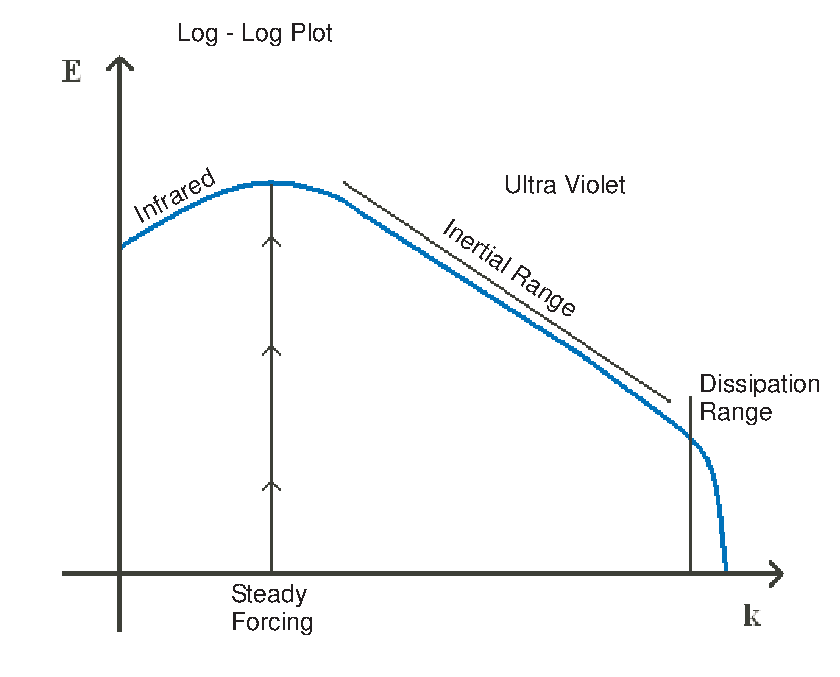
\includegraphics[width=4in]{intro_energyspectrum.eps}
   \end{center}
  \caption{Sketch of an energy spectrum. (eps file)} \label{fig: intro energy spectrum}
\end{figure}
The reason for using the double logarithmic scales is that some parts of the spectrum obey power laws and thus become straight lines in Figure \ref{fig: intro energy spectrum}.  In particular, the inertial range obeys a power law with slope $-5/3$ or nearly so.  The $-5/3$ value was obtained theoretically by Kolmogorov 1941 via a scaling argument together with his four-fifth's law \cite{Kolmogorov}.  Experimental evidence \cite{Frisch, Grant, Champagne} has confirmed an inertial range with slope near $-5/3$.

\section{Moments of the Inertial Range}

To study the inertial range, moments of various quantities are employed.  The energy spectrum is just one example of an inertial range moment obeying a power law; other examples include $\langle |\hat{u}(\vec{k})|^p\rangle$.  There is a transform specifically designed to deal with moments, namely, the Mellin transform.  It is related to the more familiar Fourier and Laplace transform through various manipulations in the complex plane; see \cite{Sneddon}.

\subsection{Mellin Transforms}

The Mellin transform is defined as
\begin{equation}
      \Phi(z) = \mathcal{M}[\phi(x);z] \equiv \int_{0}^{\infty}x^{z-1}\phi(x)\ dx. \label{eq:mellin}
\end{equation}
When $\phi(x)$ is a probability density function of a \emph{positive} random variable $X$,
\begin{equation}
    \phi(x)dx = Pr\{x<X<x+dx\}, \quad x>0,
\end{equation}
then the moments of $X$ are
\begin{equation}
    \langle X^{p}\rangle = \int^{\infty}_{0}x^{p}\phi(x)dx.
\end{equation}
Next, we introduce $x$ into the equation so that we may write moments in terms of Mellin transforms;
\begin{eqnarray}
    & = & \int^{\infty}_{0}x^{p+1}\phi(x)\frac{dx}{x} \nonumber \\
    & = & \mathcal{M}[\phi(x);p+1]. \label{eq: moments of chi}
\end{eqnarray}
Since the random variable is positive, moments of non-integer orders are readily defined\footnote{We can also use Mellin transforms for a random variable that is only real rather than positive.   To do this, we split $\phi$ unto its odd and even parts.  Each part can then be treated similarly to (\ref{eq: moments of chi}).}.  The only restriction on $p$ is that the improper integral must converge.  The function $\phi$ is then uniquely determined from its moments through the inverse Mellin transform. It, like the inverse Laplace transform, involves a contour integral in the complex plane.

In order to use the Mellin transform in our investigations, it is necessary that we know how various self-similarities transform.  Suppose, our pdf, $\phi$, depends parametrically on a length scale, $\ell$, i.e. $\phi = \phi(x,\ell)$, in a self-similar way where $\ell = 2\pi/k$.  For example, we could have
\begin{equation}
    \phi(x,\ell) = C(\ell)f\left( \frac{x}{\sigma(\ell)}\right), \label{eq: self similar ex}
\end{equation}
where $\sigma = \langle X^{2}\rangle^{1/2}$ and $f(x) \geq 0$, represents the similarity profile.  Of course, $C$ would then be specified by the requirement that $\phi(x,\ell)$ be a pdf, i.e.
\begin{eqnarray}
    \int^{\infty}_{0}\phi(x,\ell)dx = & C\int^{\infty}_{0}f\left(\frac{x}{\sigma(\ell)}\right)dx & = 1 \\
    \Rightarrow C = & \left( \sigma\int^{\infty}_{0}f(u)du\right)^{-1} & = \sigma^{-1}.
\end{eqnarray}
For the Mellin transform, we then have
\begin{eqnarray}
    \mathcal{M}[\phi(x;\ell);z] & = & C\mathcal{M}\left[f\left(\frac{x}{\sigma}\right);z \right] \nonumber \\
    & = & C\sigma^{z}\mathcal{M}[f(x);z] \nonumber \\
    & = & \sigma^{z-1}\frac{F(z)}{F(1)}
\end{eqnarray}
where $F(z) = \mathcal{M}[f(x);z]$ and $F(1) = 1$ only if $f(x)$ is a pdf.

Correspondingly, we have
\begin{equation}
    \langle X^{p} \rangle = \mathcal{M}[\phi(x;\ell); p+1] = \frac{\sigma^{p}(\ell)F(p+1)}{F(1)}
\end{equation}
and
\begin{equation}
    \langle X \rangle^{p} = \mathcal{M}[\phi(x;\ell); 2]^{p} = \left(\frac{\sigma(\ell)F(2)}{F(1)}\right)^{p},
\end{equation}
so that the dimensionless ratio
\begin{equation}
    \frac{\langle X^{p} \rangle}{\langle X \rangle^{p}} = \frac{F(p+1)}{F(1)}\left(\frac{F(2)}{F(1)}\right)^{p} \label{eq: dimensionless ratio}
\end{equation}
is independent of $\ell$.  The self-similarity (\ref{eq: self similar ex}), also known as global scaling invariance or statistical self-similarity, was used by Kolmogorov as a postulate in his 1941 theory to obtain the $-5/3$ slope \cite{Kolmogorov}. From (\ref{eq: dimensionless ratio}) it follows that the corresponding exponents are linear, i.e. if $\langle X^{p}\rangle = C_{p}\ell^{\zeta_{p}}$ then $\zeta_{p} = p\zeta_{1}$.

\section{Scaling Exponents}

In the inertial range, the moments of almost any numerical value one can think of are power laws in the scale.  When working in Fourier space the magnitude of the wave number $|\vec{k}|$ defines the scale.  However, not all theoretical investigations use Fourier space.  The Karmon-Howarth equation \cite{Hinze}, for example, works with a spatial length scale.  This equation, formulated in the thirties, uses two point spatial correlations for the reason that these are readily obtained experimentally.  Specifically, velocity differences between two points depend only on the separation distance $\ell$ when the turbulence is homogeneous and isotropic.  Only two velocity differences come into play: $\delta v_{\parallel}(\ell)$ and $\delta v_{\perp}(\ell)$.  The former is parallel to the line segment connecting the two points, the latter perpendicular to it.  For the second order moments, e.g. $\langle (\delta v_{\parallel})^2\rangle$, a direct connection can be established with Fourier space through Parseval's identity.  For other orders there is, unfortunately, no similar connection.

The four-fifth's law of Kolmogorov in 1941 was formulated in terms of $\delta v_{\parallel}(\ell)$.  This states
\begin{equation}
    \langle (\delta v_{\parallel})^3\rangle = -\frac{4}{5} \epsilon \ell
\end{equation}
where $\epsilon$ is the dissipation. Combining the four-fifth's-law with the assumption of statistical self-similarity (\ref{eq: self similar ex}), he readily obtained
\begin{equation}
    \langle (\delta v_{\parallel})^p\rangle = C_p\ell^{\zeta_p} = \tilde{C}_p\epsilon^{p/3}\ell^{p/3}
\end{equation}
with $\zeta_p = \zeta_3\dot p/3 = p/3$, where $C_p$ are supposedly universal coefficients.  This scaling law is commonly called K41.  Note $\zeta_p$ is a linear function of $p$.  The -5/3 slope of the energy spectrum is a direct consequence of K41.  The idea of universal coefficients soon was questioned by Landau \cite{Frisch}.  Since the sixties it also has become clear that the scaling exponents $\zeta_p$ are nonlinear, which is referred to as anomalous scaling and is often associated with intermittent fluctuations.

Experimental evidence \cite{Anselmet, Noullez, VanAtta, Vincent} conclusively shows that $\zeta_p$ is nonlinear, but also show that the four-fifth's law is valid.  There have been many attempts at modeling the anomalous scaling.  Kolmogorov in 1962 suggested that $\zeta_p$ should be quadratic in his log normal theory.  By using a matched asymptotic expansion Lundgren has produced a model in which K41 and anomalous scaling results are present \cite{Lundgren}.  The moments are given as an integral that depends on a function $f(q)$, where $f(q)$ has a peak close to $q = 1/3$.  If $q = 1/3$, then K41 is produced.  However, if $q<1/3$, then anomalous scaling is produced \cite{Lundgren}.  Another model that mimics observed scaling exponents is the Log-Poisson model of She and Leveque \cite{She}.  They argue that the moment ratios create a universal relationship between consecutive structures. This in turn led to the scaling exponents we use in Chapter \ref{ch:log poisson scaling}.  The data that came from the experiment done by \cite{Anselmet} was the foundation for another model.  After observing their data, Parisi and Frisch decided to weaken the global scale-invariance of K41 and use a local scale-invariance \cite{Parisi}. Each of these models produces anomalous scaling.

\section{Methods for Obtaining Data from the Inertial Range}

In order to study the inertial range, we need to obtain numerical data.  There are at least three different approaches one can take: physical experiments \cite{YakhotNASA}; direct numerical simulations of the Navier Stokes equations \cite{Moser}; and numerical studies of models of the Navier Stokes equations \cite{Frisch}. There are advantages and shortcomings to each approach.  In the physical experiment all the effects of Navier Stokes equations are, of course, present in real form.  However, homogeneous and isotropic turbulence  is an idealization which can only be approximated in an experimental facility.  Moreover, the data may not be obtainable in the form one would like.  In particular, experiments usually provide time series of velocity increments $\delta v_{\parallel}$ and $\delta v_{\perp}$ for various separations whereas one would like to known the Fourier decomposition of the velocity.

Direct numerical simulations of the Navier Stokes equations do provide the Fourier decomposition but at limited Reynolds numbers.  It is difficult to have high resolution in the entire inertial range and still have an adequate dissipation range.  The periodic box effect, inherent in the usual spectral codes, is also a problem at the larger scales.  In spite of these shortcomings, direct numerical simulations are undoubtedly the best at providing data.  The computational resources are, however, well outside the range of what is reasonable for this thesis.

For this reason, we resort to studying models of Navier Stokes equations in wave number space.  Such models are known as shell models and allow us to consider very high Reynolds numbers.  In fact, the limit of infinite Reynolds numbers is approachable.  Moreover, the computational resource requirements are modest.

\section{Organization of the Chapters}

In Chapter \ref{ch:strectched exponentials} will we explore the use of stretched exponentials as functions to describe inertial range pdf's.  However, we find that this class of functions fail because they do not admit for power law scaling in the inertial range.
Chapter \ref{ch:log poisson scaling} investigates pdf's constructed from given scaling exponents.  In particular, we look at the log Poisson model of anomalous scaling \cite{She}. We find that the pdf has a number of strange and undesirable features.
Chapter \ref{ch:an analytical example of self similar anomalous scaling} presents an analytic example of a pdf that is self-similar yet satisfies the power law requirement with nonlinear exponents.  This provides a specific example that anomalous scaling may be expressed through self-similarity; an idea that was believed to have sunk with K41.  This is a specific example from the new theory proposed in \cite{Melander2007}.
Chapter \ref{ch:shell models} introduces the shell models which will be used to generate inertial range data for our analysis in subsequent chapters. Shell models are severe truncations of the Navier Stokes equations in Fourier space.  We chose two specific models; GOY and Sabra, both are well known. Both shell models are crudely analogous to spectral Navier Stokes equations \cite{Ditlevsen, Mogensen}.
In Chapter \ref{ch:conservation laws}, we prove that the inviscid invariants, energy and helicity, are conserved for the truncated version of each model when the viscosity and forcing vanish. The truncated versions are what we actually solve numerically.
Chapter \ref{ch:numerical simulations} carries out the numerical simulations on each model and investigates how viscosity effects the results and the duration of a simulation.  We also introduce structure functions, scaling laws, scaling exponents, and characteristic length scales.
In Chapter \ref{ch:self similarity of the joint pdf}, we look at the pdf for the time series of each shell variable.  In particular, we show how the data in the inertial range can be collapsed using a similarity transformation.  Furthermore, we inspect how well the power laws hold for each model.
Chapter \ref{ch:a new theory} reviews a new self-similarity theory built on the observed collapse of the data in Chapter \ref{ch:self similarity of the joint pdf}. The functional equation for the pdf emerges from the theoretical analysis.
Discarding the GOY model, Chapter \ref{ch: before the theory}, then applies the new theory to the data from the Sabra shell model.
Chapter \ref{ch:conclusion} wraps up the analysis of the theory and the shell model. 




\chapter{Background} 
\label{ch:background}

In this chapter, we describe the background of our research, 
including the basic technology related to this work and the 
hardware/software tools that we used to implement and evaluate 
our proposed algorithms in this work.


\section{White Space Bands}

The white space band term is mentioned the frequencies channels 
previously used by analog TV broadcasts. In United States, full 
power analog television broadcasts, which operated between the 
54 MHz and 806 MHz television frequencies (Channels 2-69), ceased 
operating on June 12, 2009 per a United States digital switchover 
mandate. At that time, full power TV stations were required to 
switch to digital transmission and operate only between 54 MHz 
and 698 MHz.~\cite{fccwhitespace} 

Industry and academia have recognized the value of white space 
bands in wireless communication. Various proposals, including 
IEEE 802.11af, IEEE 802.22 and those from the White Spaces 
Coalition, have advocated using white spaces left by the termination 
of analog TV to provide wireless broadband Internet access. Some 
company from industry has designed device intended to use these 
new available channels as a "white-spaces device" (WSD), such as 
Ubiquiti SR serials products. These devices are designed to detect 
the presence of existing but unused areas of airwaves, such as 
those reserved for analog television, and utilize these unused 
airwaves to transmit signals for data traffic. Such technology 
is predicted to improve the availability of broadband Internet 
service, especially in rural areas.

White space bands and ISM WiFi bands have great variation of 
propagation characteristics. Wireless propagation refers to 
the signal loss characteristics when wireless signals are 
transmitted through the wireless medium. The strength of the 
received signal depends on both the line-of-sight path (or lack 
thereof) and multiple other paths that result from reflection, 
diffraction, and scattering from obstacles~\cite{andersen1995propagation}. 
The widely-used Friis equation characterizes the received signal 
power $P_r$ in terms of transmit power $P_t$, transmitter gain 
$G_t$, receiver gain $G_r$, wavelength $\lambda$ of the carrier 
frequency, distance $R$ from transmitter to receiver, and path 
loss exponent $n$ according to~\cite{friis}:

\begin{equation}
\label{eq:friis}
P_r=P_t+G_t+G_r+10n \log_{10}\left( \frac{\lambda}{4\pi R}\right)
\end{equation}
Here, $n$ varies according to the aforementioned environmental 
factors with a value ranging from two to five in typical outdoor 
settings~\cite{rappaport}.

According to Eq.~\ref{eq:friis} white space band not only provide more 
bandwidth for wireless communication, but also bring the diversity in 
transmission/interference range. Our algorithms and frameworks try to 
exploit white space bands advantages of link communication and network 
deployment through spectrum agility with WiFi bands.


\section{Spectrum Utilization}

When access a channel licensed by FCC, most of the time we could detect signals in the 
air from devices who share the channel. To represent the utilization level of a channel, 
we define \emph{activity level}, $A$, as the percentage of time when the channel is 
occupied by all competing sources $x_j (j = 1, 2, 3, ...)$ other than the intended 
transmitter $y$. For 802.11-based transmissions, the activity level on band $i$ is 
defined as:
\begin{equation}
\label{eqn:80211activity}
A^i = \frac{\sum_j{\sum_k{\frac{L_k^{x_j}}{R_k^{x_j}}}}}{\sum_k{\frac{L_k^y}{R_k^y}}+\sum_j{\sum_k{\frac{L_k^{x_j}}{R_k^{x_j}}}}+S\sigma}
\end{equation}
where $L_k^{x_j}$ and $R_k^{x_j}$ represent the packet length in bits and data
rate at which that packet is transmitted, for external sources $x_j$;
$S$ and $\sigma$ are the number of idle slots and slot duration, respectively. 
When considering the activity level of non-802.11 users 
({\it e.g.}, the bands currently licensed to TV),
we use the received signal level from non-802.11 interfering sources $P_N^i$ 
on band $i$ directly as an input to our algorithms. 


% Talk about the available channel
In practical, we get the activity level through in-field measurements.
The measurements process will be introduced in following chapters.
We define the percentage of sensing samples ($S_\theta$) above an 
interference threshold ($\theta$) over the total samples ($S$) in a time unit as the 
activity level ($A$) of inter-network interference:
\begin{equation}
\label{eq:actdef}
A=\frac{S_\theta}{S_a}
\end{equation}
The capacity of a clean channel is denoted by $C$. With the protocol model, the capacity 
of a channel with inter-network interference $C_r$ could be represented as 
the remaining free time of the channel capacity according to: 
\begin{equation}
\label{eq:intercap}
C_r=C*(1-\bar{A})
\end{equation}


\section{Gateworks Platform}

The off the shelf platform we use for our measurements is the GW2358. 
GW2358 is a member of the Gateworks Cambria Single Board Computer family. 
The GW2358 meets the requirements for enterprise and residential network 
applications. This single board computer consists of an Intel IXP435 XScale 
operating at 667MHz, 128Mbytes of DDRII-400 DRAM, and 32Mbytes of Flash. 
Peripherals include four Type III Mini-PCI sockets, two 10/100 Base-TX 
Ethernet ports with IEC-6100-4 ESD and EFT protection, two USB Host ports, 
and Compact Flash socket. Additional features include digital I/O, serial 
EEPROM, real time clock with battery backup, system monitor to track 
operating temperature and input voltage, RS232 serial port for management 
and debug, and watchdog timer. The GW2358 also supports GPS and RS485 
serial port as ordering options. Power is applied through a dedicated 
connector or through either Ethernet connector with the unused signal 
pairs in a passive power over Ethernet architecture. 
An open source software OpenWrt board support package is included 
for Linux operating systems.


\begin{figure} 
%\vspace{-0.1in}
\centering
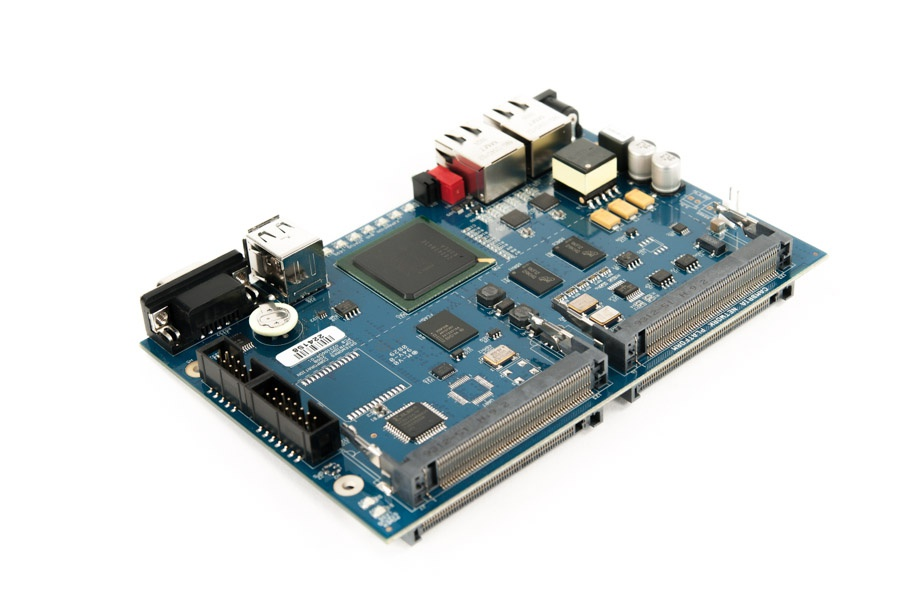
\includegraphics[width=75mm]{figures/gw2358}
\vspace{-0.1in}
\caption{The Gateworks GW2358 off-shelf Platform.}
\label{fig:gw2358}
\vspace{0.1in}
\end{figure}



The Gateworks platform works with Ubnt radios to perform 802.11 
multiband measurements for both indoor and in-field. It helps to 
collect the SNR, throughput and packet information for the post 
process. 

\section{Rohde \& Schwarz FSH8 Spectrum Analyzer}

The R\&S FSH 8 spectrum analyzer is designed portable for application 
in multiple environment, especially for in-field measurement. Its low 
weight, its simple, well-conceived operation concept and the large number 
of measurement functions make it an indispensable tool for anyone who 
needs an efficient measuring instrument for outdoor work. We employ 
FSH 8 in our indoor and outdoor measurements to collect data in multiple
bands.

\begin{figure} 
%\vspace{-0.1in}
\centering
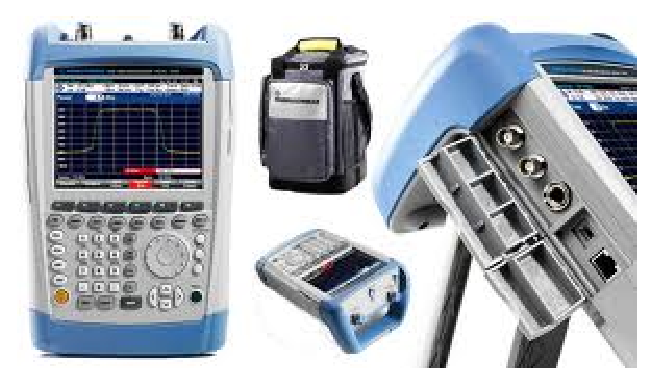
\includegraphics[width=75mm]{figures/fsh8}
\vspace{-0.1in}
\caption{Rohde \& Schwarz FSH 8 Spectrum Analyzer.}
\label{fig:fsh8}
\vspace{0.1in}
\end{figure}

FSH 8 is able to sense the signal in the air from 9 KHz to 
8 GHz. The spectrum analyzer could sense both 802.11 signals 
and non-802.11 signal in the air. Through the time stamp, 
we could merge data from Gateworks platform and FSH8 platform 
to perform our algorithms and frameworks.

\section{Mesh Network Deployment}

Wireless Mesh Network is the infrastructure to provide 
wireless access for clients by the vendors. Wireless 
mesh network is made up of radio nodes organized in a mesh 
topology. Each node forwards messages on behalf of the 
other nodes. The nodes connected to clients are counted 
as the access tier, the nodes to relay data traffic to 
wired networks are backhual tier. For access tier, the 
nodes need to cover the service area and provide enough 
capacity for the clients in the service area. The backhual 
tier need to have high efficient connection to the wired 
network. We analyze the mesh network deployment in multiband 
scenario, and propose our solution for access and backhual 
network deployment.



%\section{Multiband Adaptation}
\label{sec:model}
In this section, we first formulate the multiband 
adaptation problem in vehicular wireless links and introduce the set of information we use to make band decisions, which we refer to as context information. We then propose two machine-learning-based 
multiband adaptation algorithms for vehicular channels. For comparison, we also propose two baseline adaptation methods based on existing solutions which consider historical and instantaneous information independently.

\subsection{Problem Formulation}
%The focus of this paper is on a context-based multiband adaptation algorithm as:
%The problem we are going to resolve is to find a band has the best throughput in multiple available options as:
Consider a system with~$n$ frequency bands, represented by an index set~$\{1,2, \ldots, n\}$. 
The objective is to select the optimal band,~$b_{best}$, to transmit at each time instant that maximizes a desired objective function such as throughput. The throughput~$r_i$ on band~$i$ depends on several factors such as received signal power~$P_R^i$, noise power~$P_N^i$, the channel busy time~$B^i$, the velocity of the transmitter,~$v_{tx}$,
 the velocity of the receiver,~$v_{rx}$, 
 and location information which depends on each algorithm and will be specified in the algorithm section. The aforementioned set of all information used to make multiband decisions composes the users context. 
 %Add Context
% Context is the information that can represent the characters of a wireless user.For mobile wireless users, velocity, RSSI, interference and location could be counted as context information.
This relationship is represented in general as~$r_i = f(P_R^i, P_N^i, B^i, v_{tx}, v_{rx}, $context information per algorithm$)$. The objective can be stated as:
\begin{equation}
b_{best}= \arg \max_i r_i 
\end{equation}
%\begin{align}
%\label{eqn:estimation}
%f: (v_{tx}, v_{rx},  P_R^1,..., P_R^n, B^1, ..., B^n,P_N^1,..., P_N^n,) \rightarrow b_{best}
% \end{align}
%where $v_{tx}$ and $v_{rx}$ are the velocities of the transmitter and the receiver, 
%$P_R^i$ is the received power, $P_N^i$ is the non-802.11 interfering signal level and
 %Why we use context information 
%$B^i$ is the \emph{busy time}. 
The framework differentiates interference from other nodes using the same technology (via the busy time $B^i$) and other technologies (via the noise level~$P_N^i$). For instance, an 802.11 node can decode the packets of other 802.11 nodes but can only sense
instantaneous noise levels from ZigBee/Bluetooth nodes. 
Decoding the packets can provide increased knowledge such as 
data rate and packet size to determine the duration of the channel use.
%To help make decisions for multiband adaptation in a similar context,
We can exploit the long-term behavior by using historical performance
data for the collected context information
({\it e.g.}, $v_{tx}$, $v_{rx}$, $B^i$, $P_N^i$, $P_R^i$)~\cite{meikle2012global}. 
%can be used by people tending to have repeatable patterns
%~\cite{meikle2012global} and we could improve the performance with each trip 
%to the region if we could passively observe context along this repeatable 
%pattern. The variables used in each algorithm will be explained for each algorithm 
%later. 


To represent the utilization level of the channel, we define \emph{busy time}, $B$,
as the percentage of time when the channel is occupied by 
all competing sources $x_j (j = 1, 2, 3, ...)$ other than the intended transmitter $y$. 
For 802.11-based transmissions, the busy time on band $i$ is defined as:
\begin{equation}
\label{eqn:80211activity}
B^i = \frac{\sum_j{\sum_k{\frac{L_k^{x_j}}{R_k^{x_j}}}}}{\sum_k{\frac{L_k^y}{R_k^y}}+\sum_j{\sum_k{\frac{L_k^{x_j}}{R_k^{x_j}}}}+S\sigma}
\end{equation}
where $L_k^{x_j}$ and $R_k^{x_j}$ represent the packet length in bits and data
rate at which that packet is transmitted, for external sources $x_j$;
$S$ and $\sigma$ are the number of idle slots and slot duration, respectively. 
When considering the activity level of non-802.11 users 
({\it e.g.}, the bands currently licensed to TV),
%and other non-802.11 devices), 
%whether the signal level from these
%competing sources reaches a level to disrupt communication at the receiver
%would define a similar notion of busy time. However, since this depends
%on the environment, hardware, coding, and modulation level, 
we use the received signal level from non-802.11 interfering sources $P_N^i$ 
on band $i$ directly as an input to our algorithms. 

\subsection{Multiband Adaptation Algorithms}
\label{subsec:algorithms}
%2 baseline methods: 
%1. band selection based on identifying the the most common class, 
%2. SNR-based band selection
In order to evaluate the proposed multiband adaptation algorithms, 
we construct two baseline methods: (i.) We search for the
most commonly selected band as the best band in the historical data
and choose it as the final band decision. (ii.) For each band, we build 
a lookup table for throughput $T_{ideal}$ in an idealized channel given the $RSSI$ and obtain 
the best band according to following:
\begin{align}
&\max_i T_{ideal}^i\times(1-B^i),
\label{eq:baseline2}
\end{align}
The throughput $T_{ideal}$ is measured with an Azimuth ACE-MX channel emulator~\cite{AzimuthACE}. 
The details of the system setup and data collection are discussed in Section~\ref{sec:experiment design}. 

Machine learning has been used as an important tool in wireless communications~\cite{haykin2005cognitive}. When a user enters an area, the machine
learning algorithm can learn from the historical data and
select the potential optimal band given the input, {\it e.g.}, $P_R^i$, $v$
and $P_N^i$. We propose two multiband adaptation algorithms based on
two machine learning methods: k-nearest neighbor (KNN) and decision trees.

%2 machine learning methods: 
%1. modified KNN, 

{\bf Location-based Look-up Algorithm.} KNN is a machine learning method
based on searching for the closest training data points in the feature space and various
modified versions have been applied successfully for classification~\cite{zhang2006svm}.
In the {\it Location-based Look-up Algorithm}, we search for the closest neighbors of 
a testing point by using each parameter one by one in the input set. 
The {\it Location-based Look-up Algorithm} additionally involves geographic information for band selection other than received signal power~$P_R^i$, noise power~$P_N^i$, the activity/occupancy level~$B^i$, the velocity of the transmitter,~$v_{tx}$.
The 
performance of the selected training data points is averaged to generate an estimate of the performance at each band. Then
the band with the highest throughput performance is selected as $b_{best}$.
%comparing with machine learning algorithms. 

For the {\it Location-based Look-up Algorithm}, 
context information involves the location $g$ (GPS latitude and longitude), $v$, $P_R^i$, $P_N^i$ 
and $B^i$. To make a band prediction, we have four look-up blocks to reduce
the training data points which are similar to the testing data point. First,
we search for the historical data which is closest to the testing data based on GPS location.
If the number of found historical data points is less than a predefined threshold, 
 $\theta_{AArea}$, we increase the distance range (the actual threshold is discussed in 
Section~\ref{sec:experiment design}). Then, based on the filtered historical data,
we collect $\theta_{AArea}$ data points which are closest to $P_R^i$, where $\theta_{AArea}$ is the threshold of the number of collected data points. 
A similar process is repeated based on $P_N^i$ and $v$, respectively.
After deciding the final data set, we average the throughput of data points at each band.
This algorithm's key steps are shown in Algorithm~\ref{algorithms: Location}.
%At last, the average throughput of the most similar data will be adjust of the 802.11 
%\emph{busy time} and tell the best band.


%\begin{algorithm}
%\small
%\caption{Location-based Look-up Algorithm}
%\begin{algorithmic}[1]
%	  \REQUIRE  ~~\\
%		  $g$: Location information of multiband node\\
%		 $ \theta_{Area}$: Threshold of a location\\
%		 $\theta_{RSSI}$: Threshold of RSSI\\
%		 $\theta_{Velocity}$: Threshold of velocity\\
%		 $\theta_{A Area}$: Threshold of data amount for a location\\
%		 $\theta_{A RSSI}$: Threshold of data amount for RSSI\\
%		 $\theta_{A Non 802.11 SI}$: Threshold of data amount for non-802.11 interference\\
%		 $\theta_{A Velocity}$: Threshold of data amount for velocity\\
%		 $D^i \in \{D^1,D^2,\dots,D^n\}$: Historical look-up data
%\ENSURE ~~\\    
%$b_{best}$: Optimal transmission band
%\FOR    {$i<=n$}
%\STATE Initialize \emph{$Data_{Location}, Data_{RSSI}, Data_{Velocity}$} to zero matrix;
%\WHILE {$Amount(Data_{Location,i})<\theta_{A Area}$}
%\STATE $Data_{Location,i} \leftarrow f_{Lookup}(D^i,g,\theta_{Area})$: Find data in $D^i$ whose distance less than $\theta_{Area}$;
%\STATE $\theta_{Area}=\theta_{Area} \times 1.1$;
%\ENDWHILE
%
%\WHILE {$Amount(Data_{RSSI,i})<\theta_{A RSSI}$}
%\STATE $Data_{RSSI,i} \leftarrow f_{Look-up}(D_{Location,i},P_R^i,\theta_{RSSI})$: Find data in $D_{Location}$ the RSSI similar to $P_R^i$ in range $\theta_{RSSI}$;
%\STATE $\theta_{RSSI}=\theta_{RSSI} \times 1.1$;
%\ENDWHILE
%
%\WHILE {$Amount(Data_{P_N,i})<\theta_{A Non 802.11 SI}$}
%\STATE $Data_{RSSI,i} \leftarrow f_{Look-up}(D_{Location,i},P_N^i,\theta_{RSSI})$: Find data in $D_{Location}$ the RSSI similar to $P_N^i$ in range $\theta_{RSSI}$;
%\STATE $\theta_{A Non 802.11 SI}=\theta_{A Non 802.11 SI} \times 1.1$;
%\ENDWHILE
%
%\WHILE {$Amount(Data_{Velocity,i})<\theta_{A Velocity}$}
%\STATE $Data_{Velocity,i} \leftarrow f_{Lookup}(D_{RSSI,i},v,\theta_{Velocity})$: Find data in $D_{RSSI}$ the RSSI similar to $v$ in range $\theta_{RSSI}$;
%\STATE $\theta_{Velocity}=\theta_{Velocity} \times 1.1$;
%\ENDWHILE \\
%
%\STATE $T_{a,i}=avr(Data_{Velocity,i})$;
%\STATE  $T_{e,i}=T_a^i\times(1-B^i)$;
%\ENDFOR \\  
%\STATE $b_{best} = \max_i\{T_e^1,\dots,T_e^i,\dots,T_e^n\}$;\\
%\end{algorithmic}
%\label{algorithms: Location}
%\end{algorithm}

%2. region-based C4.5 (different region sizes)
{\bf Region-based Decision Tree Algorithm.} Decision trees are a  
widely-used machine learning 
algorithm due to their low complexity and stable performance~\cite{banfield2007}.
A decision tree can model the relationship in the training data between the context 
information and the optimal band as a set of tree-like deduction structures. Before 
implementing the training process, we prepare a training set including a group of 
training data points of $\{v_{tx}, v_{rx}, P_R^1, ..., P_R^n,  B^1, ..., B^n, P_N^1, 
..., P_N^n, b_{best}\}$ based on the collected measurements. We obtain $b_{best}$ by comparing
the throughput performance of all available bands and selecting the band with the highest 
throughput. We choose the C4.5 algorithm to generate our decision tree~\cite{hall2009weka}, a widely-used algorithm based on the 
information entropy gain. 

At each intermediate
node in the decision tree, the learning algorithm calculates the information entropy 
gain of splitting the remaining training data points based on each parameter in the input 
set, {\it e.g.}, $P_R^i$, $v$ or $P_N^i$. Then, it compares and selects the parameter with 
the highest entropy gain to decide the test condition at each intermediate node until 
all training data points are classified.  The leaf nodes indicate the optimal band for 
prediction in our application. Then, the trained decision structure is integrated into 
the transmitter protocol stack. With the collected context information, the decision 
structure can suggest the band with the best throughput performance. 

The relationship between the context information and the best band could differ at
different locations because of diverse propagation environment characteristics. 
To reduce the heterogeneity of training data from different locations, we split 
the vehicular route into several regions and implement the training process based 
on the historical data collected in each region. Then, the trained decision structure 
is integrated in our system for multiband adaptation in each region. The granularity 
of regional division is one parameter that affects the training set as well as the 
performance of the resulting decision tree. We 
evaluate the granularity of these divisions in Section~\ref{sec:experiment design}.

%\begin{algorithm}                      % enter the algorithm environment
\caption{Calculate $y = x^n$}          % give the algorithm a caption
\label{alg1}                           % and a label for \ref{} commands later in the document
\begin{algorithmic}                    % enter the algorithmic environment
    \REQUIRE $n \geq 0 \vee x \neq 0$
	    \ENSURE $y = x^n$
		    \STATE $y \Leftarrow 1$
			    \IF{$n < 0$}
				        \STATE $X \Leftarrow 1 / x$
						        \STATE $N \Leftarrow -n$
								    \ELSE
									        \STATE $X \Leftarrow x$
											        \STATE $N \Leftarrow n$
													    \ENDIF
														    \WHILE{$N \neq 0$}
															        \IF{$N$ is even}
																	            \STATE $X \Leftarrow X \times X$
																				            \STATE $N \Leftarrow N / 2$
																							        \ELSE[$N$ is odd]
																									            \STATE $y \Leftarrow y \times X$
																												            \STATE $N \Leftarrow N - 1$
																															        \ENDIF
																																	    \ENDWHILE
																																		\end{algorithmic}
																																		\end{algorithm}


%\chapter{Vehicular Link Spectrum Adapatation} 
\label{ch:vnc}

%
\section{Introduction}
\label{sec:introduction}


%Background
%Worldwide governments and societies are active to achieve road safety and travel comfort of drivers and passengers.
Drivers and passengers around the world could utilize a wide array of vehicular applications ranging from real-time traffic monitoring and
safety applications to various {\it infotainment} applications.
%spanning news, weather, audio, and video streams.  
However, the continuous use of such applications is limited due to the challenge of transmitting over 
highly-dynamic vehicular wireless channels. 
In such networks, the increasing availability of different 
frequency bands with correspondingly diverse propagation characteristics could allow flexibility and 
robustness of vehicular links. Even with spectral flexibility, links are extremely tenuous, 
demanding instantaneous decisions to remain connected, motivating an algorithm that
can find the appropriate frequency band quickly and according to the current environmental context.

Cognitive radio mechanisms which interleave channel accesses also motivate the frequency
band selection problem of finding the optimal spectrum on which to 
transmit~\cite{ghasemi2008spectrum}.
%Furthermore, in existing systems, there are a number of different technologies from which to choose and the demand of
% integrating the advantages of multiple protocol is presented as Heterogeneous Wireless Networks has opening topics related to band selection~\cite{hossain2010vehicular}.
Prior work has considered a number of challenges in
leveraging white space frequencies including spectrum sensing, frequency-agile operation,
geolocation, solving stringent spectral mask requirements, and providing reliable service
in unlicensed and dynamically changing spectrum~\cite{shellhammer2009technical}. In particular, there has recently been an acceleration
in spectrum sensing work~\cite{rayanchu2011fluid, kim1996pulse,cabric2004implementation}. Based on 
these works, protocols have been built for multi-channel and/or multiband wireless operation~\cite{MOAR,
raychaudhuri2003spectrum,sabharwal2007opportunistic}.  Other works have presented methods for searching for the most efficient 
transmission channel~\cite{mo2005comparison}, discovering channel information~\cite{rayanchu2011fluid, sabharwal2007opportunistic}, and estimating 
channel quality~\cite{MOAR}.
Finally, the emergence of a number of diverse sensors on a vehicle motivates work
on heterogeneous wireless networks, which have different frequency bands {\it and}
technologies~\cite{hossain2010vehicular}. Thus, the various communication 
standards have diverse throughput capacity, allowing the choice of technology 
to possibly usurp frequency band decisions. For example, an 802.11n link at 5.8 
GHz with high levels of loss
might still be a better choice than a Bluetooth link at 2.4 GHz with little loss
due to the discrepancy of hundreds of Mbps in throughput capacity.
%To consider the choice of frequency band, band selection problem for htereogeneous wireless networks should be researched under the same protocol, which make it similar to our problem~\cite{hossain2010vehicular}.
%Add heterogeneous and cognitive radio
%Research of heterogeneous wireless networks has been done for these purpose in Roadside-to-Vehicle and Vehicle-to-Vehicle.\cite{hossain2010vehicular}.
%the understanding of primary/secondary users adaptation\cite{cordeiro2007c}, combining multiple devices for vehicle~\cite{hossain2010vehicular}.

However, for the purposes of this work, we assume the underlying technology is the same to evaluate the choice of frequency band.
While these works have considered spectral activity and developing protocols and algorithms to 
find spectral holes, less of a focus has been on coupling such information with historical performance in a given 
propagation environment.
In this paper, 
we develop multiband adaptation protocols which couple the prior knowledge of in-situ performance of various bands with the instantaneous knowledge of 
spectral activity, SNR, and current location of each band to arrive at a decision on the optimal band to transmit. To do so, we use an
off-the-shelf platform that allows direct comparison and simultaneous experimentation across four different wireless
frequency bands from 450 MHz to 5.8 GHz with the same physical
and media access layers. 
%changes that frequency differences of hundreds of MHz to GHz could have on the band %decision. Moreover, it is well known that propagation greatly depends on the environment %in operation~\cite{rappaport}.  Thus, knowledge of the environment in operation could %allow the relationship between received power differences across multiple frequency bands %to have much greater accuracy.  

%Contributions  fixme
The main contributions of our work are as follows:
\begin{itemize}
\item We first develop a framework for multiband adaptation using both historical information and instantaneous measurements. This framework is broad enough to study adaptation across licensed and unlicensed bands, including white space frequency bands.  

\item We propose two different machine-learning-based multiband adaptation algorithms. The 
first machine learning algorithm, referred to as the \emph{Location-based 
Look-up Algorithm}, 
is based on the idea of $k$-nearest-neighbor classification. The second machine-learning-based 
algorithm uses \emph{decision trees} for classification. 
For comparison, we also create two baseline adaptation algorithms which attempt to make the optimal band selection based on only: (i.)~historical 
performance data, and (ii.)~instantaneous SNR measurements across 
various bands. 

%We consider four different algorithms for comparison.  First, we consider a scheme
%in which the throughput is achieved on an emulated channel for
%the current received signal level. We then adjust the predicted best band choice according to the current activity
%level (real-time information). 
%Second, we consider an approach based on machine learning which
%considers prior throughput for a given received signal and activity level
%combination.  
%Third, we build a scheme which include the prior relationship of throughput, received signal level and context information in an look up table for repeatable travel in an area.
%Fourth, we split the area to different regions and apply machine learning in each region to get the property band selection.

%earning in addition to the received signal and activity level.
%Third, we consider a second machine learning approach which considers user
%location in addition to the received signal and activity level.

\item We perform extensive outdoor V-2-V experiments to evaluate the proposed algorithms.
Our results indicate that the proposed machine learning based algorithms improve
throughput by up to $49.3\%$ over these baseline methods.

\end{itemize}



%The remainder of this paper is organized as follows. In Section II, we present the multiband adaptation problem and proposed algorithms. Section III discusses experimental evaluation of the multiband algorithms. We conclude in Section IV.




In this section, we first formulate a multiband 
adaptation problem in vehicular wireless links and introduce the 
information we use to make band decisions, which we refer to as use context. We then propose two machine-learning-based 
multiband adaptation algorithms for vehicular channels. For comparison, we also propose two baseline adaptation methods based on existing solutions, which consider historical and instantaneous information independently.




\section{Link Adaptation Problem Formulation}
%The focus of this paper is on a context-based multiband adaptation algorithm as:
%The problem we are going to resolve is to find a band has the best throughput in multiple available options as:

Consider a system with~$n$ frequency bands, represented by an index set~$\{1,2, \ldots, n\}$. 
The objective is to select the optimal band,~$b_{best}$, to transmit at each time instant that maximizes a desired objective function such as throughput. The throughput~$r_i$ on band~$i$ depends on several factors such as received signal power~$P_R^i$, noise power~$P_N^i$, the channel activity level~$A^i$, the velocity of the transmitter,~$v_{tx}$,
 the velocity of the receiver,~$v_{rx}$, 
 and location information which depends on each algorithm and will be specified in the algorithm section. The aforementioned set of all information used to make multiband decisions composes the users context. 
 %Add Context
% Context is the information that can represent the characters of a wireless user.For mobile wireless users, velocity, RSSI, interference and location could be counted as context information.
This relationship is represented in general as~$r_i = f(P_R^i, P_N^i, A^i, v_{tx}, v_{rx}, $context information per algorithm$)$. The objective can be stated as:
\begin{equation}
b_{best}= \arg \max_i r_i 
\end{equation}
The framework differentiates interference from other nodes using the same technology (via the Activity level $A^i$) and other technologies (via the noise level~$P_N^i$). For instance, an 802.11 node can decode the packets of other 802.11 nodes but can only sense
instantaneous noise levels from ZigBee/Bluetooth nodes. 
Decoding the packets can provide increased knowledge such as 
data rate and packet size to determine the duration of the channel use.
%To help make decisions for multiband adaptation in a similar context,
We can exploit the long-term behavior by using historical performance
data for the collected context information
({\it e.g.}, $v_{tx}$, $v_{rx}$, $A^i$, $P_N^i$, $P_R^i$)~\cite{meikle2012global}. 
%can be used by people tending to have repeatable patterns
%~\cite{meikle2012global} and we could improve the performance with each trip 
%to the region if we could passively observe context along this repeatable 
%pattern. The variables used in each algorithm will be explained for each algorithm 
%later. 


%To represent the utilization level of the channel, we define \emph{activity level}, $A$,
%as the percentage of time when the channel is occupied by 
%all competing sources $x_j (j = 1, 2, 3, ...)$ other than the intended transmitter $y$. 
%For 802.11-based transmissions, the activity level on band $i$ is defined as:
%\begin{equation}
%\label{eqn:80211activity}
%A^i = \frac{\sum_j{\sum_k{\frac{L_k^{x_j}}{R_k^{x_j}}}}}{\sum_k{\frac{L_k^y}{R_k^y}}+\sum_j{\sum_k{\frac{L_k^{x_j}}{R_k^{x_j}}}}+S\sigma}
%\end{equation}
%where $L_k^{x_j}$ and $R_k^{x_j}$ represent the packet length in bits and data
%rate at which that packet is transmitted, for external sources $x_j$;
%$S$ and $\sigma$ are the number of idle slots and slot duration, respectively. 
%When considering the activity level of non-802.11 users 
%({\it e.g.}, the bands currently licensed to TV),
%we use the received signal level from non-802.11 interfering sources $P_N^i$ 
%on band $i$ directly as an input to our algorithms. 

\section{Multiband Adaptation Algorithms}
\label{subsec:algorithms}

In order to evaluate the proposed multiband adaptation algorithms, 
we construct two baseline methods: (i.) We search for the
most commonly selected band as the best band in the historical data
and choose it as the final band decision. (ii.) For each band, we build 
a lookup table for throughput $T_{ideal}$ in an idealized channel given the $RSSI$ and obtain 
the best band according to following:
\begin{align}
&\max_i\ T_{ideal}^i\times(1-A^i),
\label{eq:baseline2}
\end{align}
The throughput $T_{ideal}$ is measured with an Azimuth ACE-MX channel emulator~\cite{AzimuthACE}. 
The details of the system setup and data collection are discussed in Section~\ref{sec:vncexperimentdesign}. 

Machine learning has been used as an important tool in wireless communications~\cite{haykin2005cognitive}. When a user enters an area, the machine
learning algorithm can learn from the historical data and
select the potential optimal band given the input, {\it e.g.}, $P_R^i$, $v$
and $P_N^i$. We propose two multiband adaptation algorithms based on
two machine learning methods: k-nearest neighbor (KNN) and decision trees.

%2 machine learning methods: 
%1. modified KNN, 

{\bf Location-based Look-up Algorithm.} KNN is a machine learning method
based on searching for the closest training data points in the feature space and various
modified versions have been applied successfully for classification~\cite{zhang2006svm}.
In the {\it Location-based Look-up Algorithm}, we search for the closest neighbors of 
a testing point by using each parameter one by one in the input set. 
The {\it Location-based Look-up Algorithm} additionally involves geographic information for band selection other than received signal power~$P_R^i$, noise power~$P_N^i$, the activity/occupancy level~$A^i$, the velocity of the transmitter,~$v_{tx}$.
The 
performance of the selected training data points is averaged to generate an estimate of the performance at each band. Then
the band with the highest throughput performance is selected as $b_{best}$.
%comparing with machine learning algorithms. 

For the {\it Location-based Look-up Algorithm}, 
context information involves the location $g$ (GPS latitude and longitude), $v$, $P_R^i$, $P_N^i$ 
and $A^i$. To make a band prediction, we have four look-up blocks to reduce
the training data points which are similar to the testing data point. First,
we search for the historical data which is closest to the testing data based on GPS location.
If the number of found historical data points is less than a predefined threshold, 
 $\theta_{AArea}$, we increase the distance range (the actual threshold is discussed in 
Section~\ref{sec:vncexperimentdesign}). Then, based on the filtered historical data,
we collect $\theta_{AArea}$ data points which are closest to $P_R^i$, where $\theta_{AArea}$ is the threshold of the number of collected data points. 
A similar process is repeated based on $P_N^i$ and $v$, respectively.
After deciding the final data set, we average the throughput of data points at each band.
This algorithm's key steps are shown in Algorithm~\ref{algorithms: Location}.


\begin{algorithm}
\caption{Location-based Look-up Algorithm}
\label{algorithms: Location}
\begin{algorithmic}[1]
\REQUIRE  ~~\\
	 $g$: Location information of multiband node\\
	 $\theta_{Area}$: Threshold of a location\\
	 $\theta_{RSSI}$: Threshold of RSSI\\
	 $\theta_{Velocity}$: Threshold of velocity\\
	 $\theta_{set} = \{\theta_{A Area},\theta_{A RSSI},\theta_{A Non 802.11 SI},\theta_{A Velocity}\}$: Threshold of data amount for \{a location, RSSI, non-802.11 interference, velocity\}\\
%	 $\theta_{A Area}$: Threshold of data amount for a location\\
%	 $\theta_{A RSSI}$: Threshold of data amount for RSSI\\
%	 $\theta_{A Non 802.11 SI}$: Threshold of data amount for non-802.11 interference\\
%	 $\theta_{A Velocity}$: Threshold of data amount for velocity\\
	 $D^i \in \{D^1,D^2,\dots,D^n\}$: Historical look-up data
\FOR    {$i<=n$}
\STATE Initialize \emph{$Data_{Location}, Data_{RSSI}, Data_{Velocity}$} to zero matrix;


\FOR {$j<=m$}
\STATE $Amount = Amount_{\{Data_{Location,i},Data_{RSSI,i},Data_{P_N,i},Data_{Velocity,i}\}}^j$;
\STATE $\theta = \theta_{set}^j$;
\WHILE {$Amount<\theta$}
\STATE $Data_{Location,i} \leftarrow f_{Lookup}(D^i,g,\theta_{Area})$: Find data in $D^i$ whose distance less than $\theta_{Area}$;
\STATE $\theta_{Area}=\theta_{Area} \times 1.1$;
\ENDWHILE

%\WHILE {$Amount(Data_{RSSI,i})<\theta_{A RSSI}$}
%\STATE $Data_{RSSI,i} \leftarrow f_{Look-up}(D_{Location,i},P_R^i,\theta_{RSSI})$: Find data in $D_{Location}$ the RSSI similar to $P_R^i$ in range $\theta_{RSSI}$;
%\STATE $\theta_{RSSI}=\theta_{RSSI} \times 1.1$;
%\ENDWHILE
%
%\WHILE {$Amount(Data_{P_N,i})<\theta_{A Non 802.11 SI}$}
%\STATE $Data_{RSSI,i} \leftarrow f_{Look-up}(D_{Location,i},P_N^i,\theta_{RSSI})$: Find data in $D_{Location}$ the RSSI similar to $P_N^i$ in range $\theta_{RSSI}$;
%\STATE $\theta_{A Non 802.11 SI}=\theta_{A Non 802.11 SI} \times 1.1$;
%\ENDWHILE

%\WHILE {$Amount(Data_{Velocity,i})<\theta_{A Velocity}$}
%\STATE $Data_{Velocity,i} \leftarrow f_{Lookup}(D_{RSSI,i},v,\theta_{Velocity})$: Find data in $D_{RSSI}$ the RSSI similar to $v$ in range $\theta_{RSSI}$;
%\STATE $\theta_{Velocity}=\theta_{Velocity} \times 1.1$;
%\ENDWHILE \\

\STATE $T_{a,i}=avr(Data_{Velocity,i})$;
\STATE  $T_{e,i}=T_a^i\times(1-A^i)$;
% ENDFOR for amount and theta
\ENDFOR \\  
\ENDFOR \\  
\STATE $b_{best} = \max_i\{T_e^1,\dots,T_e^i,\dots,T_e^n\}$;\\
\ENSURE ~~\\    
$b_{best}$: Optimal transmission band
\end{algorithmic}
\end{algorithm}

%2. region-based C4.5 (different region sizes)
{\bf Region-based Decision Tree Algorithm.} Decision trees are a  
widely-used machine learning 
algorithm due to their low complexity and stable performance~\cite{banfield2007}.
A decision tree can model the relationship in the training data between the context 
information and the optimal band as a set of tree-like deduction structures. Before 
implementing the training process, we prepare a training set including a group of 
training data points of $\{v_{tx}, v_{rx}, P_R^1, ..., P_R^n,  A^1, ..., A^n, P_N^1, 
..., P_N^n, b_{best}\}$ based on the collected measurements. We obtain $b_{best}$ by comparing
the throughput performance of all available bands and selecting the band with the highest 
throughput. We choose the C4.5 algorithm to generate our decision tree~\cite{hall2009weka}, a widely-used algorithm based on the 
information entropy gain. 

At each intermediate
node in the decision tree, the learning algorithm calculates the information entropy 
gain of splitting the remaining training data points based on each parameter in the input 
set, {\it e.g.}, $P_R^i$, $v$ or $P_N^i$. Then, it compares and selects the parameter with 
the highest entropy gain to decide the test condition at each intermediate node until 
all training data points are classified.  The leaf nodes indicate the optimal band for 
prediction in our application. Then, the trained decision structure is integrated into 
the transmitter protocol stack. With the collected context information, the decision 
structure can suggest the band with the best throughput performance. 

The relationship between the context information and the best band could differ at
different locations because of diverse propagation environment characteristics. 
To reduce the heterogeneity of training data from different locations, we split 
the vehicular route into several regions and implement the training process based 
on the historical data collected in each region. Then, the trained decision structure 
is integrated in our system for multiband adaptation in each region. The granularity 
of regional division is one parameter that affects the training set as well as the 
performance of the resulting decision tree. We 
evaluate the granularity of these divisions in Section~\ref{sec:vncexperimentdesign}.

\section{Experiments for Multiband Algorithms}
\label{sec:vncexperimentdesign}

%As discussed in Section \ref{subsec:algorithms}, 
%one algorithm is applicable for entering a strange area, 3 algorithms are more appropriate for area has been visited.
To study these algorithms, we have developed indoor 
and in-field experiments on 
%an off-the-shelf wireless platform.
%Testbed and emulator Platform
%To ensure the results are broadly applicable, we employ 
a Linux-based 802.11 testbed~\cite{Openwrt}. The platform includes a 
Gateworks 2358 motherboard with Ubiquiti XR radios (XR9 at 900 MHz, 
XR2 at 2.4 GHz, XR5 at 5.2 GHz) and a DoodleLabs DL475 radio at 
450 MHz~\cite{Gateworks,Ubnt}.  We use 
an Azimuth ACE-MX channel emulator for
controllable propagation and fading characteristics with a broad range of 
industry-standard channel models from 450 MHz to 5.9 GHz~\cite{AzimuthACE}. 

%context information experiments
\subsection{In-lab Experiments for Radio Characterization}
\label{subsec:ichannel}
To establish an SNR-to-throughput relationship for the \emph{SNR-based 
Throughput Look-up Algorithm}, we use an experimental setup where two 
wireless nodes communicate across repeatable emulated channels generated 
by the channel emulator (Figure~\ref{fig:in-door experiment}). For a given band and card, we measure
the throughput of a fully-backlogged UDP flow using the {\it iperf} 
traffic generator. We use constant attenuation over an idealized
channel condition and repeat the experiment to
produce various RSSI values.
Despite the same physical and media access control layers of the radios, there are
slight differences in the throughput achieved per radio at the same attenuation
level.  Thus, we normalize these throughput values to have the same maximum
throughput across radio types.
%for a fair comparison of the frequency bands.

\begin{figure} [h]
%\vspace{-0.1in}
\centering
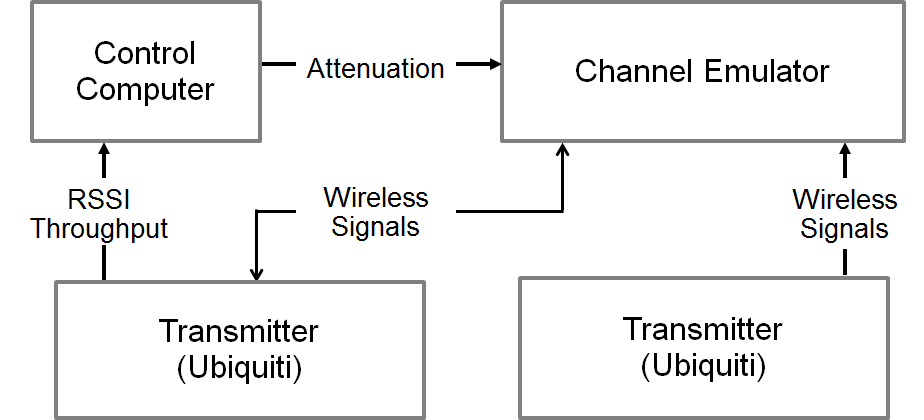
\includegraphics[width=65mm]{figures/emulator2}
%\vspace{-0.1in}
\caption{Experimental setup for channel emulator.}
\label{fig:in-door experiment}
\vspace{-0.1in}
\end{figure}

%\subsection{Signal Level Context-aware information}
\subsection{Experimental Design for In-field Data Collection}
\label{subsec:insitu}
We now describe the in-field experimental design to obtain a data set for
evaluating our multiband algorithms. Two Gateworks boards, each containing
the aforementioned four radios, are installed on two cars.  One node is always
the receiver and at a fixed location. The other node is always the 
transmitter and travels 
around the block of a public park as shown in Figure~\ref{fig:infield}.
One loop of the route will be used as a unit of training in the next section.

\begin{figure} [h]
%\vspace{-0.1in}
\centering
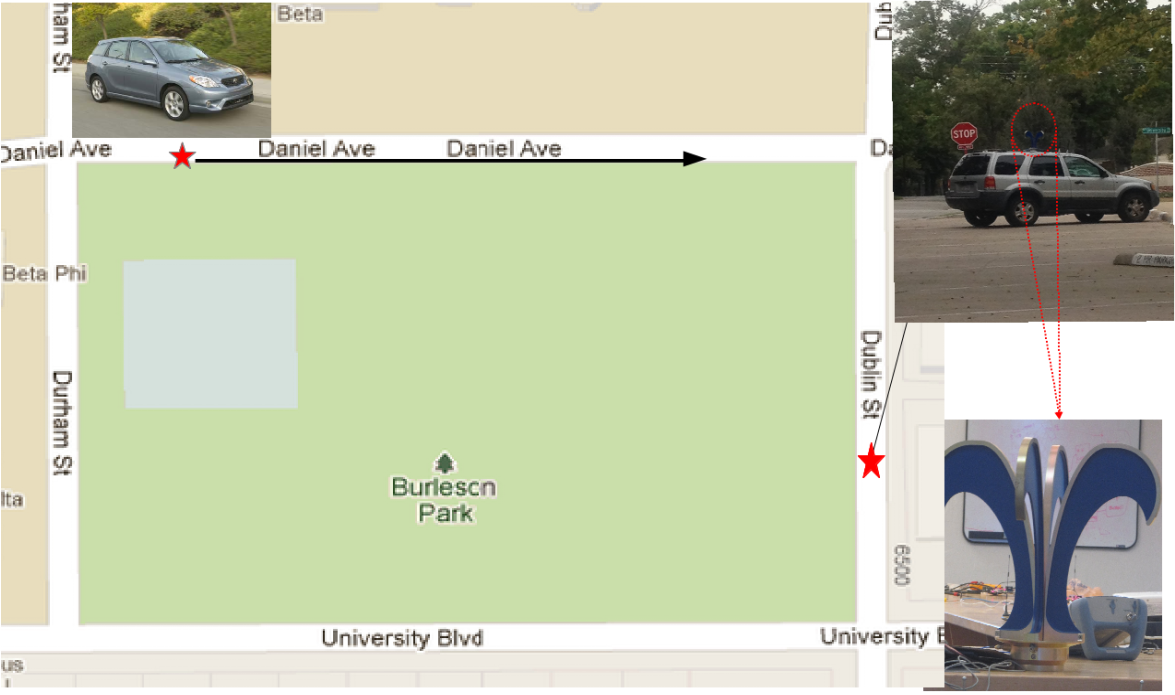
\includegraphics[width=75mm]{figures/infield}
\vspace{-0.1in}
\caption{In-field Experimental Setup.}
\label{fig:infield}
\vspace{-0.1in}
\end{figure}

During each loop, the transmitter sends a fully-backlogged UDP flow
using {\it iperf} on each of the four radios simultaneously.  To
focus on band selection and ensure the greatest range, we disable autorate and use a fixed data rate
of 6 Mbps. The receiver continually performs a {\it tcpdump} of all
received 802.11 packets~\cite{jacobson1989tcpdump}. Additionally, a
QH 400 Quad Ridge Horn Antenna (shown in Figure~\ref{fig:infield}) is 
connected to a Rhode \& Schwarz FSH8 mobile spectrum analyzer at the 
receiver to monitor spectral activity. Then, based on the 
time stamps, we remove 802.11 packets from the spectral trace 
so that only non-802.11 interference will contribute to $P_N^i$.

\begin{figure} 
%\vspace{-0.1in}
\centering
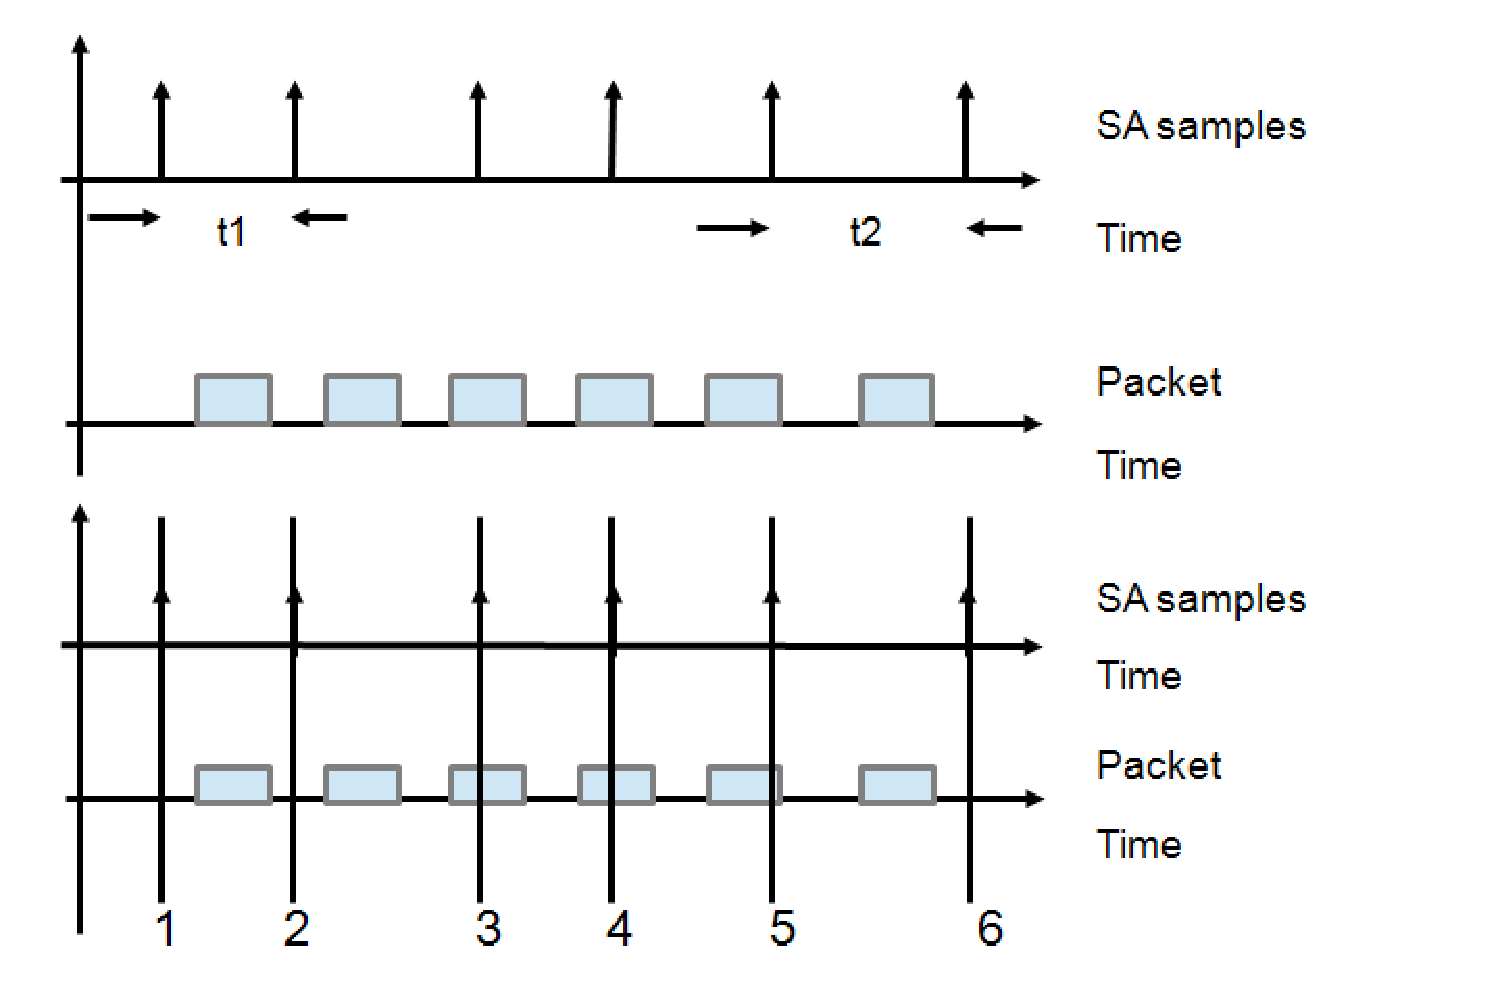
\includegraphics[width=75mm]{figures/sa_process}
\vspace{-0.1in}
\caption{Spectrum Analyzer Data Processing.}
\label{fig:sa_process}
\vspace{0.1in}
\end{figure}

Figure~\ref{fig:sa_process} shows how we obtain the
non-802.11 interference, $P_N^i$. We expunge the spectrum analyzer
(SA) samples which overlap in time with the dumped 802.11 packets,
such as packets 3, 4, and 5. Then, the reported interference value
will not contain the received power from 802.11 packets, which have
already been considered via the activity level, $A$.

The in-field data is processed offline where data from all instruments
involved is synchronized based on the GPS time stamps. 
As discussed in Section~\ref{subsec:ichannel}, the throughput of each radio
is normalized based upon emulator experiments to account for any
manufacturing differences.


\subsection{Performance Analysis of Algorithms}
\label{subsec:data process}

We now evaluate our proposed
algorithms with the experimental setup described in
Sections~\ref{subsec:ichannel} and \ref{subsec:insitu}.
The metrics of
{\it Accuracy} and {\it Throughput Gap} are used in the evaluation.
We consider each second of the in-field trace and
observe the frequency band that had the highest 
throughput.  The \emph{Accuracy} is defined as the percentage of 
best band predictions that match the observed optimal band, where a prediction
is made each second.  Conversely, the \emph{Throughput Gap} is defined
as the difference between the throughput observed on the optimal band
and the throughput achieved by the predicted best band over the
throughput of the observed optimal band. 
In the situation where the optimal band is not chosen, the throughput could be close between the chosen and optimal bands, meaning that the
incorrect band choice did not result in a large throughput loss. Thus, the 
\emph{Throughput Gap} metric captures the severity of the incorrect choice.

%\begin{align}
%\label{equation:df accuracy}
%Accuracy = \frac{Correct\ Prediction\ Slots}{All\ Predict\ Time\ Slots}
%\end{align}
%
%\emph{Throughput Gap} is the deference between the performance of estimation throughput and measured best throughput as defined in Formula \ref{equation:df gap}.
%
%\begin{align}
%\label{equation:df gap}
%Throughput\ Gap = \frac{\sum{Max\ Tpt- Estimate\ Band\ Tpt}}{\sum{Max\ Tpt}}
%\end{align}

Since the \emph{SNR-based Throughput Look-up Algorithm} requires only 
emulator-based training, the \emph{Accuracy} and \emph{Throughput Gap} can 
be calculated for all loops of the in-field trace.  However, the 
\emph{Location-based Look-up Algorithm} and \emph{Region-based Decision
Tree Algorithm} require in-field training. Thus, the data set must be
divided into a training set and testing set for evaluation.

\begin{figure}
%\vspace{-0.0in}
\centering
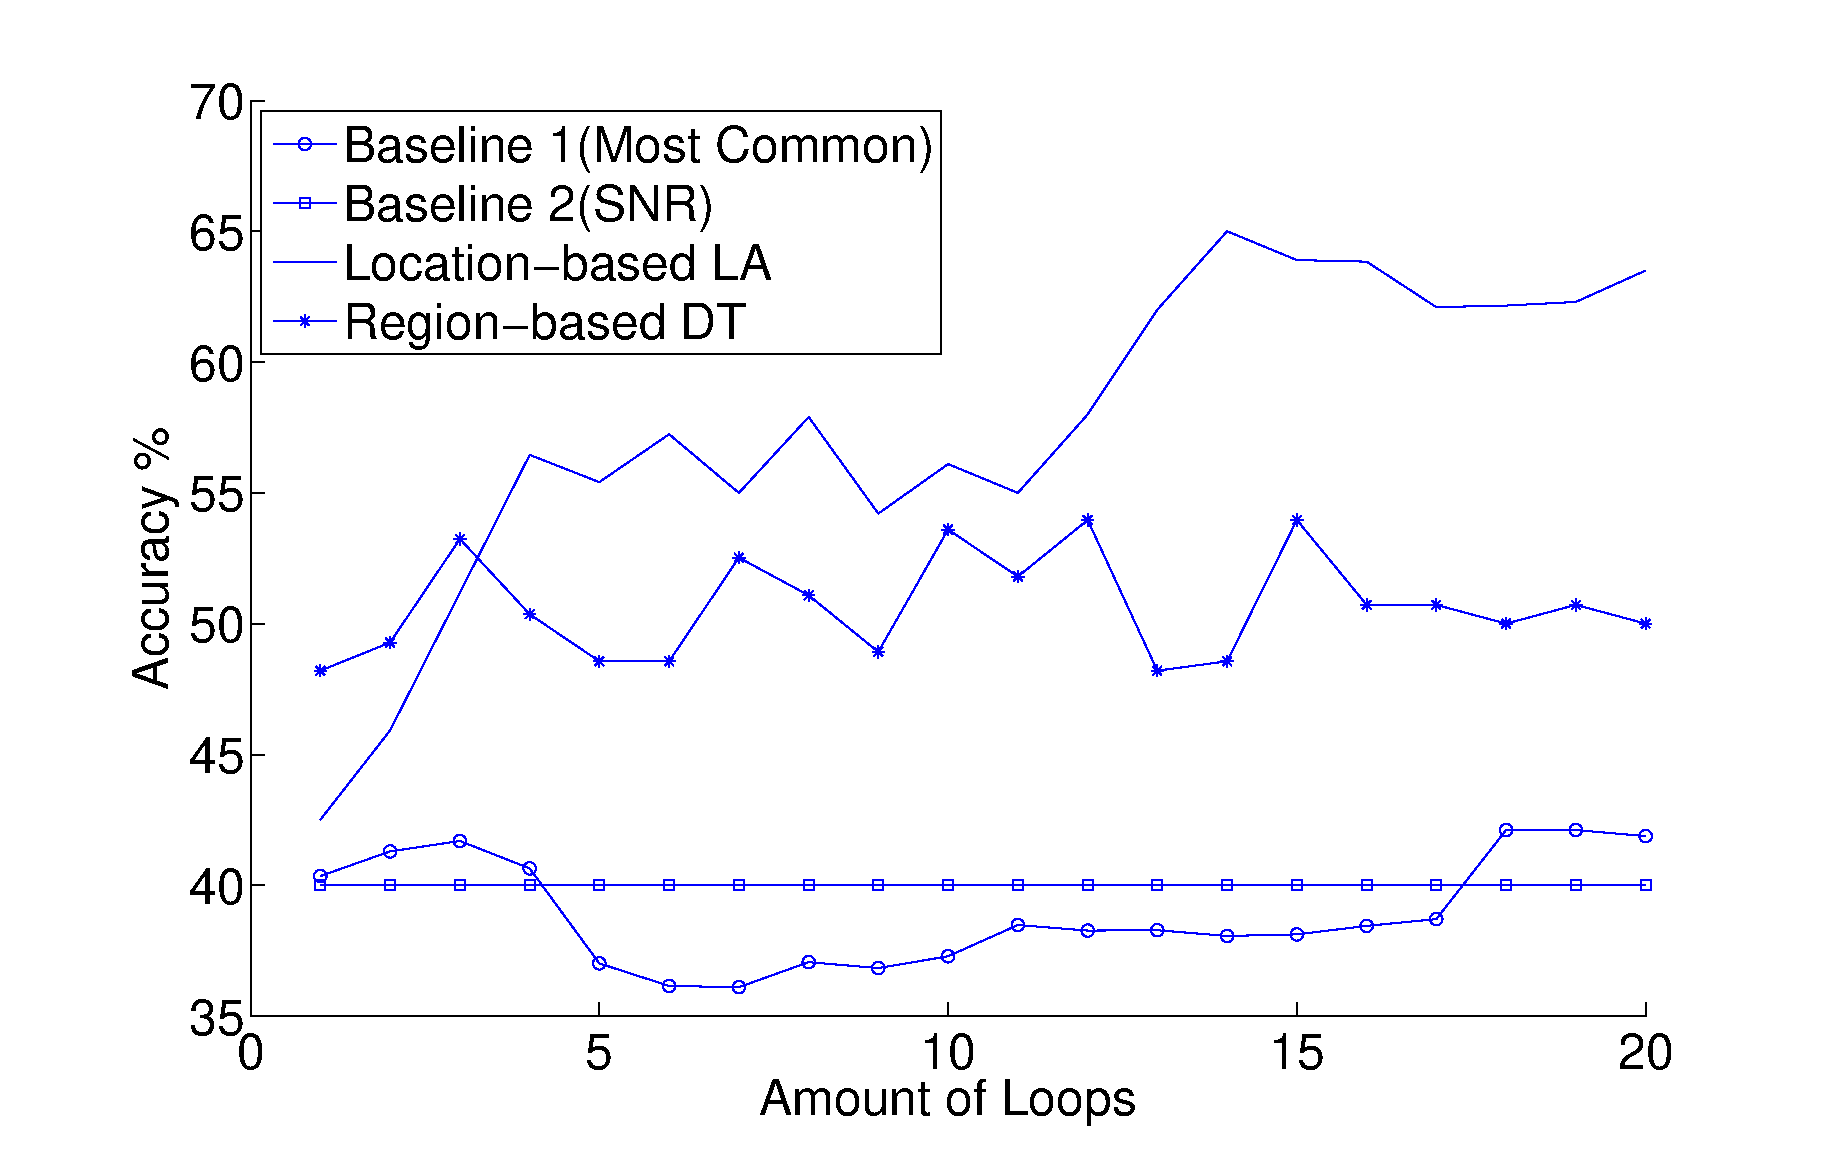
\includegraphics[width=68mm]{figures/performance_accuracy}
\vspace{-0.1in}
\caption{Accuracy of the four multiband algorithms.}
\label{fig:performance}
%\vspace{-0.0in}
\end{figure}

In Figure \ref{fig:performance}, we show the aforementioned \emph{Accuracy}
of the four multiband algorithms in selecting the band with the highest
throughput. The x-axis represents the number of loops around the
block of the mobile transmitter (shown in 
Figure~\ref{fig:infield}) that will be used by the machine-learning-based
algorithms. We use the same training and testing set to compare 
the \emph{Location-based Look-up Algorithm} and \emph{Region-based
Decision Tree Algorithm}. From the results, we observe the following:

\begin{itemize}
\item
At each loop, the first baseline algorithm, \emph{Most Commonly-Selected
Band}, uses the band with the greatest long-term average of the percentage
of time that band yields the highest throughput over the previous loops.
The accuracy ranges from 36.1\% to 42.9\%.
\item
The second baseline algorithm, \emph{SNR-based Throughput Look-up},
maintains 39.2\% across all the loops since it relies only on 
emulator-based training.
\item 
The \emph{Region-based Decision Tree Algorithm} has an accuracy ranging
from 48.2\% to 54.0\% but contains many dips due to the relationship
between the context information and the distribution of the best band
choice changing on a loop-by-loop basis. Additional training data 
slightly improves the decision structure overall but primarily induces
additional noise in the training process.
\item 
The \emph{Location-based Look-up Algorithm} begins with an accuracy of
42.5\% but improves the most out of any algorithm to finish with an 
accuracy 62.5\% with the highest accuracy of 65.0\% occurring after loop 14.
Additional in-field training loops are likely to further improve the multiband
selection accuracy.
\end{itemize}

\begin{figure}
\vspace{-0.1in}
\centering
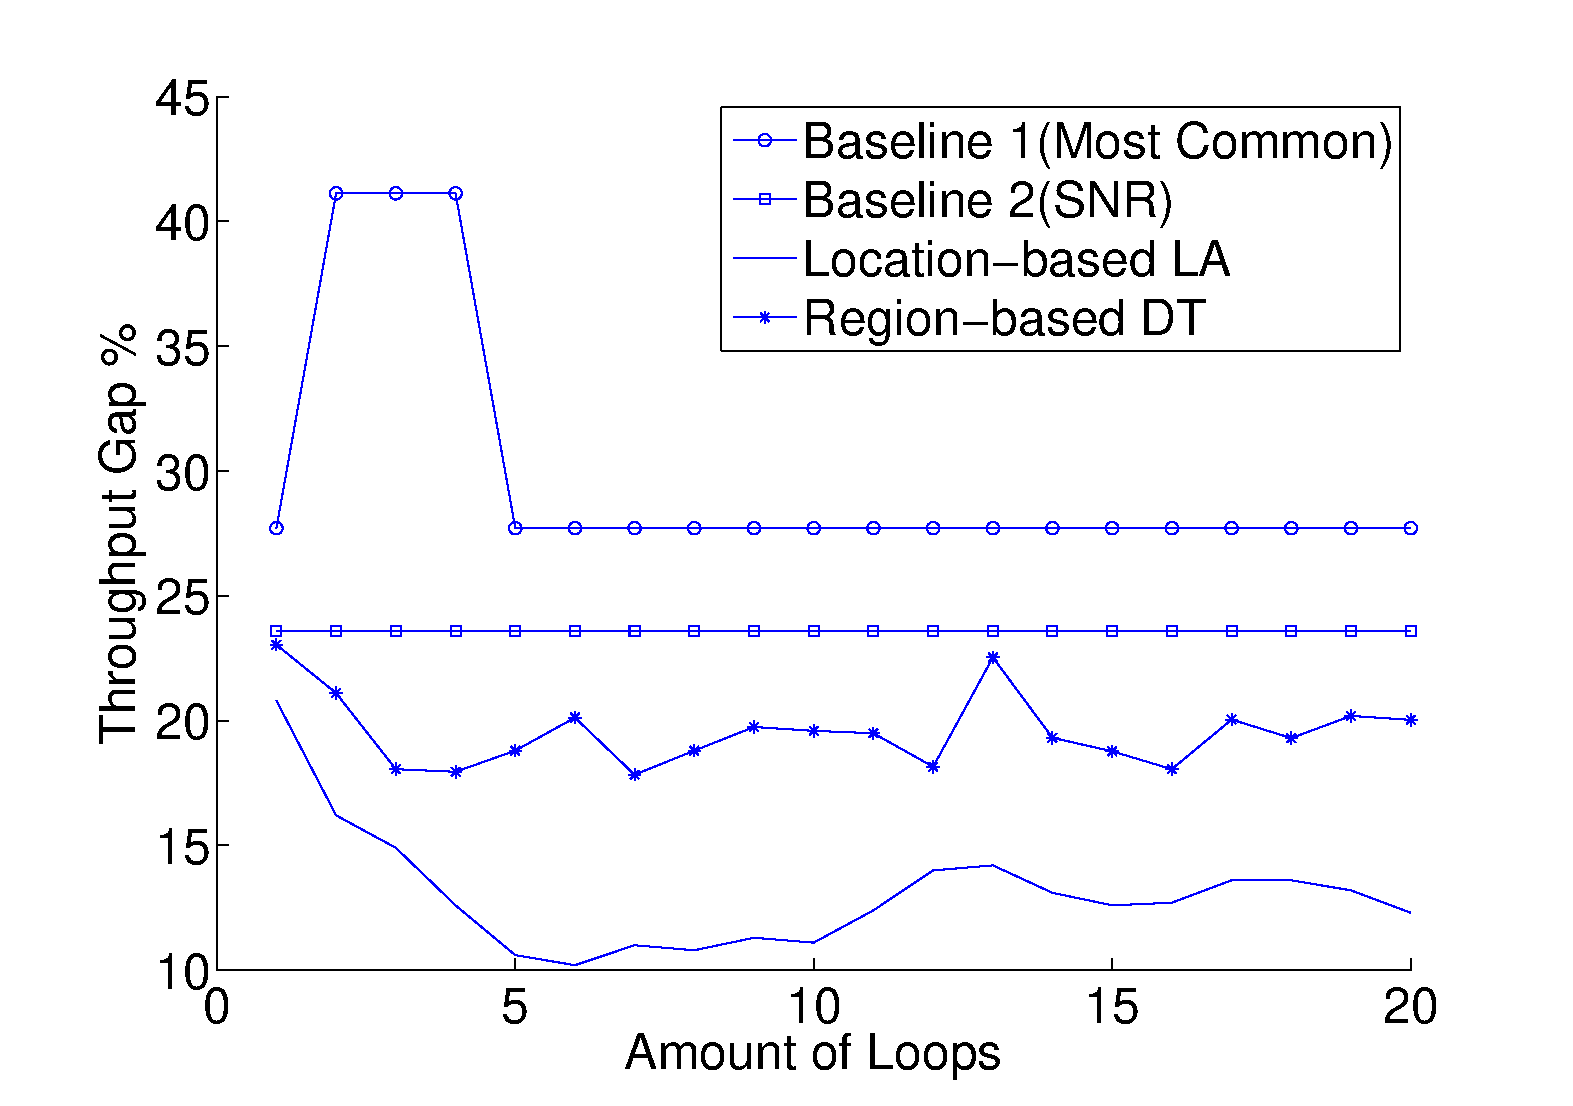
\includegraphics[width=65mm]{figures/performance_gap}
\vspace{-0.1in}
\caption{Throughput Gap of the four multiband algorithms.}
\label{fig:performance_gap}
\vspace{0.1in}
\end{figure}

Figure~\ref{fig:performance_gap}, 
depicts the \emph{Throughput Gap} of the four algorithms we evaluated and shows the following.

\begin{itemize}
\item
The \emph{Most Commonly-Selected Band Algorithm} has two different modes
of throughput gap based upon which band has the highest long-term 
percentage.  For loops 2-4, the choice is 5.8 GHz, which has a gap of 
41.1\% using the test set. For all other loops, the choice is 2.4 GHz, 
which has a gap of 27.7\%. 
\item 
The \emph{SNR-based Throughput Look-up Algorithm} shows a baseline  
performance of 23.6\% for the throughput gap.
\item 
The \emph{Region-based Decision Tree Algorithm} benefits from
additional training, going from a throughput gap of 23.0\% to 20.0\%.
Spatial and temporal changes to context information bring dips
to the curve as discussed earlier.
\item
Finally, the \emph{Location-based Look-up Algorithm} takes only 6 loops
of training to reach its lowest value of 10.2\% in terms of throughput
gap. From loops 1 to 20, the throughput gap goes from 20.8\% to 12.3\%,
which might still be improved upon with additional training.
\end{itemize}

\begin{figure}
%\vspace{-0.0in}
\centering
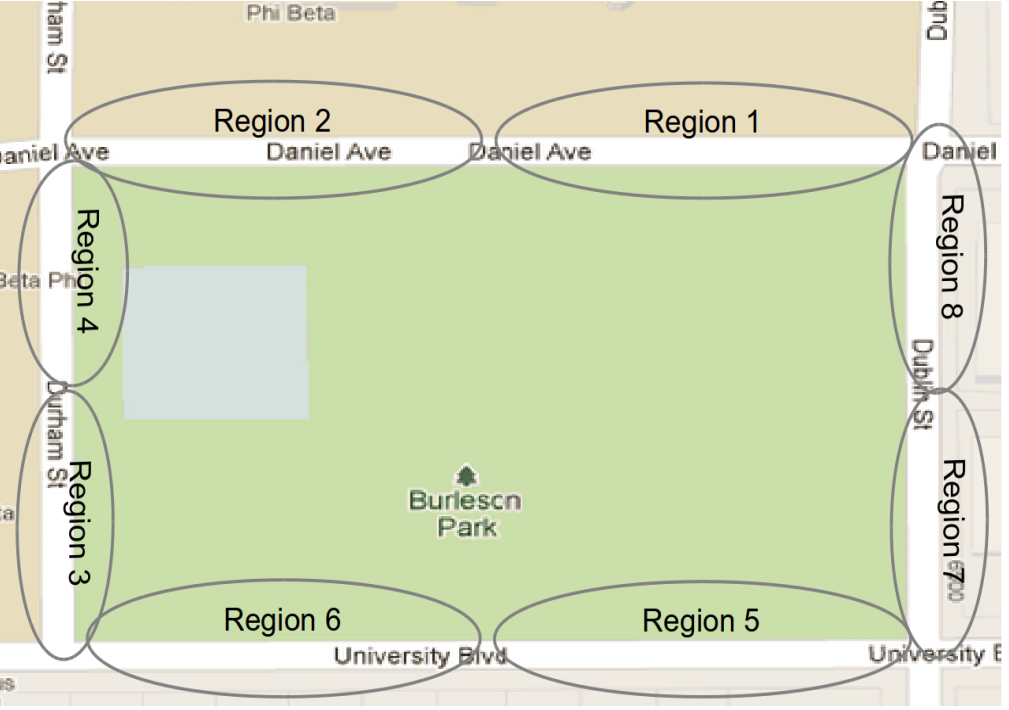
\includegraphics[width=75mm]{figures/region_map}
\vspace{-0.1in}
\caption{Spatially splitting experimental area into 8 regions.}
\label{fig:region map}
%\vspace{-0.0in}
\end{figure}

\begin{figure}
\vspace{-0.1in}
\centering
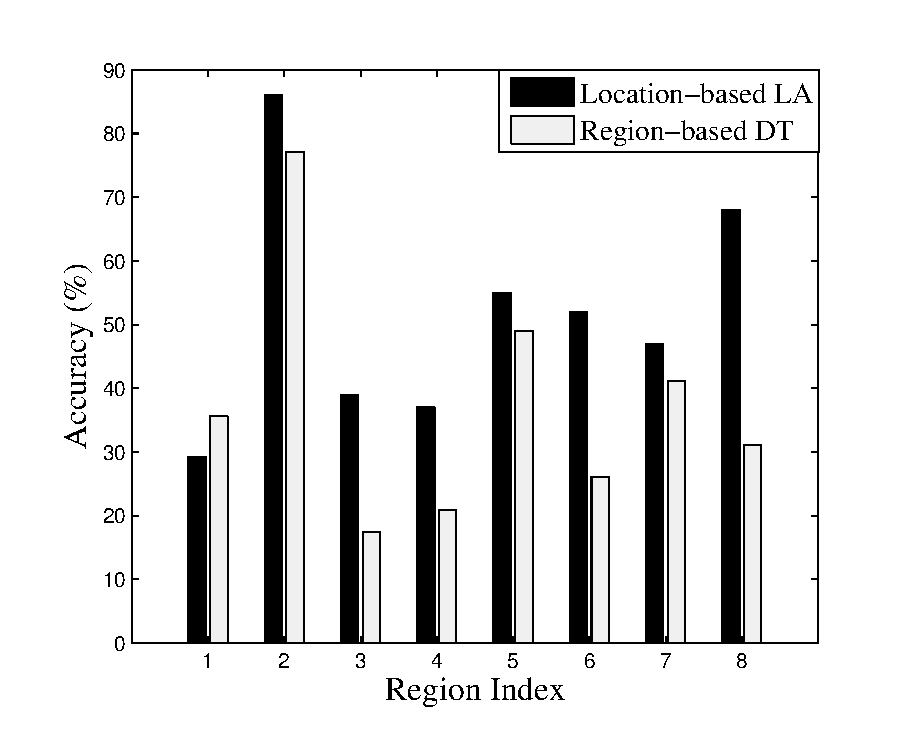
\includegraphics[width=65mm]{figures/mvsl}
\vspace{-0.1in}
\caption{Accuracy when dividing training set into 8 regions.}
\label{fig:mvsl}
\vspace{0.1in}
\end{figure}

We now consider the effect of further sub-dividing in-field experimental testing data into regions for our \emph{Location-based Look-up Algorithm} 
and \emph{Region-Based Decision Tree Algorithm}. To do so, we divide the    
loop around the park into eight regions as shown in Figure \ref{fig:region map},
which has two competing effects: (i.) Smaller regions allow similar experimental
data to be used in the training process, potentially improving the decision
structure. (ii.) For a given training set, dividing it into regions reduces
the number of training points for the machine learning algorithms, potentially
weakening the decision structure.  In Figure~\ref{fig:mvsl}, we observe 
the \emph{Accuracy} of the eight regions for both algorithms.
\begin{itemize}
\item
In all but Region 1, the \emph{Location-based Look-up Algorithm} has better 
performance than \emph{Region-based Decision Tree Algorithm}. The improved
accuracy of the former algorithm can be attributed to its ability to
distinguish each point's relative distance to the middle of the region
For the \emph{Region-based Decision Tree Algorithm}
to capture such a notion, the regions would have to be further sub-divided,
increasing the number of trees and reducing the training set per tree.
\item
For this training set, the reduction in training data caused by the
regional divisions had a net loss on the performance of the \emph{Region-based Decision Tree Algorithm}. However, if the training set was much larger
for a given area, the net effect of regional divisions could be positive.
\end{itemize}

%We have investigated the performance of the algorithms in one experimental data set and shown the gains of them. Multiband channels are complex system that knowing more information can make better decisions. 




%\section{Related Work}
\label{sec:related}

Cognitive Radio could be a powerful tool for the utility of the Spectrum Opportunity~\cite{haykin2005cognitive}.
Analog TV bands will be released for wireless communication brings opportunity to combine current wireless bands and new available bands for performance improvement employing Cognitive Radio methods~\cite{MOAR}. 


%Related research
A bunch of work has been done on radio-scene analysis and channel identification for utility of channel adaptation dating back to Simon Haykin~\cite{haykin2005cognitive}.
Some work of Multi-bands/Multi-channels in
cognitive radios focus on optimize performance, such as avoiding frequency diversity~\cite{rahul2009frequency}. 
In~\cite{OAR} an opportunistic algorithm is introduced to balance the cost of spectrum sensing, channel switching and the gain of these activities.


%Our work
Our work is motivated by prospective releasing band used for TV now and exploit the comparison across all the available bands in the future. 
It is an extension of multi-channel adaptation. 
Most of the published research focus on the stopping rules of spectrum sensing~\cite{sabharwal2007opportunistic, OAR}. In contrast, we use the data and framework to classify the performance across different bands based on the parameters we get from the context information.
%{\bf .} 


\section{Conclusion}
\label{sec:conclusion}
In this paper, we investigated multiband adaptation to leverage the propagation and context for vehicular applications. 
We did so by proposing two machine-learning-based schemes and compared their
performance against two baseline schemes.
In our experimental analysis, we evaluated the performance of these algorithms 
in the field on an off-the-shelf platform.
Experimental results demonstrate that the proposed algorithms can 
achieve up to 49.3\% greater throughput than the baseline algorithms
with an accuracy up to 65\%. In future work, we will study the impact that
multiple diverse environments have on the training as well as evaluate
the optimal use of multiple, diverse radios in unison.
%Since mobile networks have limited
%energy and training in multiple environment has not been investigated, in future work we plan to examine the influence of diverse environment and energy efficiency of
%the simultaneous use of multiple, diverse radios.



%\chapter{Spectrum Adapatation in Access Tier Network} 
\label{ch:winmee}



%
\section{Introduction}
\label{sec:introduction}


%Background
%Worldwide governments and societies are active to achieve road safety and travel comfort of drivers and passengers.
Drivers and passengers around the world could utilize a wide array of vehicular applications ranging from real-time traffic monitoring and
safety applications to various {\it infotainment} applications.
%spanning news, weather, audio, and video streams.  
However, the continuous use of such applications is limited due to the challenge of transmitting over 
highly-dynamic vehicular wireless channels. 
In such networks, the increasing availability of different 
frequency bands with correspondingly diverse propagation characteristics could allow flexibility and 
robustness of vehicular links. Even with spectral flexibility, links are extremely tenuous, 
demanding instantaneous decisions to remain connected, motivating an algorithm that
can find the appropriate frequency band quickly and according to the current environmental context.

Cognitive radio mechanisms which interleave channel accesses also motivate the frequency
band selection problem of finding the optimal spectrum on which to 
transmit~\cite{ghasemi2008spectrum}.
%Furthermore, in existing systems, there are a number of different technologies from which to choose and the demand of
% integrating the advantages of multiple protocol is presented as Heterogeneous Wireless Networks has opening topics related to band selection~\cite{hossain2010vehicular}.
Prior work has considered a number of challenges in
leveraging white space frequencies including spectrum sensing, frequency-agile operation,
geolocation, solving stringent spectral mask requirements, and providing reliable service
in unlicensed and dynamically changing spectrum~\cite{shellhammer2009technical}. In particular, there has recently been an acceleration
in spectrum sensing work~\cite{rayanchu2011fluid, kim1996pulse,cabric2004implementation}. Based on 
these works, protocols have been built for multi-channel and/or multiband wireless operation~\cite{MOAR,
raychaudhuri2003spectrum,sabharwal2007opportunistic}.  Other works have presented methods for searching for the most efficient 
transmission channel~\cite{mo2005comparison}, discovering channel information~\cite{rayanchu2011fluid, sabharwal2007opportunistic}, and estimating 
channel quality~\cite{MOAR}.
Finally, the emergence of a number of diverse sensors on a vehicle motivates work
on heterogeneous wireless networks, which have different frequency bands {\it and}
technologies~\cite{hossain2010vehicular}. Thus, the various communication 
standards have diverse throughput capacity, allowing the choice of technology 
to possibly usurp frequency band decisions. For example, an 802.11n link at 5.8 
GHz with high levels of loss
might still be a better choice than a Bluetooth link at 2.4 GHz with little loss
due to the discrepancy of hundreds of Mbps in throughput capacity.
%To consider the choice of frequency band, band selection problem for htereogeneous wireless networks should be researched under the same protocol, which make it similar to our problem~\cite{hossain2010vehicular}.
%Add heterogeneous and cognitive radio
%Research of heterogeneous wireless networks has been done for these purpose in Roadside-to-Vehicle and Vehicle-to-Vehicle.\cite{hossain2010vehicular}.
%the understanding of primary/secondary users adaptation\cite{cordeiro2007c}, combining multiple devices for vehicle~\cite{hossain2010vehicular}.

However, for the purposes of this work, we assume the underlying technology is the same to evaluate the choice of frequency band.
While these works have considered spectral activity and developing protocols and algorithms to 
find spectral holes, less of a focus has been on coupling such information with historical performance in a given 
propagation environment.
In this paper, 
we develop multiband adaptation protocols which couple the prior knowledge of in-situ performance of various bands with the instantaneous knowledge of 
spectral activity, SNR, and current location of each band to arrive at a decision on the optimal band to transmit. To do so, we use an
off-the-shelf platform that allows direct comparison and simultaneous experimentation across four different wireless
frequency bands from 450 MHz to 5.8 GHz with the same physical
and media access layers. 
%changes that frequency differences of hundreds of MHz to GHz could have on the band %decision. Moreover, it is well known that propagation greatly depends on the environment %in operation~\cite{rappaport}.  Thus, knowledge of the environment in operation could %allow the relationship between received power differences across multiple frequency bands %to have much greater accuracy.  

%Contributions  fixme
The main contributions of our work are as follows:
\begin{itemize}
\item We first develop a framework for multiband adaptation using both historical information and instantaneous measurements. This framework is broad enough to study adaptation across licensed and unlicensed bands, including white space frequency bands.  

\item We propose two different machine-learning-based multiband adaptation algorithms. The 
first machine learning algorithm, referred to as the \emph{Location-based 
Look-up Algorithm}, 
is based on the idea of $k$-nearest-neighbor classification. The second machine-learning-based 
algorithm uses \emph{decision trees} for classification. 
For comparison, we also create two baseline adaptation algorithms which attempt to make the optimal band selection based on only: (i.)~historical 
performance data, and (ii.)~instantaneous SNR measurements across 
various bands. 

%We consider four different algorithms for comparison.  First, we consider a scheme
%in which the throughput is achieved on an emulated channel for
%the current received signal level. We then adjust the predicted best band choice according to the current activity
%level (real-time information). 
%Second, we consider an approach based on machine learning which
%considers prior throughput for a given received signal and activity level
%combination.  
%Third, we build a scheme which include the prior relationship of throughput, received signal level and context information in an look up table for repeatable travel in an area.
%Fourth, we split the area to different regions and apply machine learning in each region to get the property band selection.

%earning in addition to the received signal and activity level.
%Third, we consider a second machine learning approach which considers user
%location in addition to the received signal and activity level.

\item We perform extensive outdoor V-2-V experiments to evaluate the proposed algorithms.
Our results indicate that the proposed machine learning based algorithms improve
throughput by up to $49.3\%$ over these baseline methods.

\end{itemize}



%The remainder of this paper is organized as follows. In Section II, we present the multiband adaptation problem and proposed algorithms. Section III discusses experimental evaluation of the multiband algorithms. We conclude in Section IV.


%\section{Hetergeneous Access Point Band Selection}
%\label{sec:moa_problemformulation}
%
%% Introduce the content of this section
%In this section, we illustrate the challenges of hetergenous access point 
%band selection in wireless network deployment and formulate the problem of band 
%selection in mesh network deployments jointly using WiFi and white space bands. 
%Further, we present a linear program and MHAPD(Multiband Hetergeneous AP Deployment) algorithm for estimating the 
%access point number to serve the traffic demand of a given population.
%Then we discuss the application of the algorithm in uniform population
%distribution and non-uniform population distribution with spectrum resource 
%variation to tell the general rules in picking up channels for access points.
 
%\subsection{White Space Opportunity and Challenge}
%\label{subsec:motivation}

%% Propagation
%Wireless propagation is the behavior of the signal loss characteristics 
%when wireless signals are transmitted through the wireless medium.
%The strength of the received signal depends on both the line-of-sight
%path (or lack thereof) and multiple other paths that result from 
%reflection, diffraction, and scattering from 
%obstacles~\cite{andersen1995propagation}. The widely-used Friis
%equation characterizes the received signal power $P_r$ in terms 
%of transmit power $P_t$, transmitter gain $G_t$, receiver gain $G_r$, 
%wavelength $\lambda$ of the carrier frequency, 
%distance $R$ from transmitter to receiver, and path loss exponent 
%$n$ according to~\cite{friis}:
%\begin{equation}
%\label{eq:friis}
%P_r=P_t+G_t+G_r+10n \log_{10}\left( \frac{\lambda}{4\pi R}\right)
%\end{equation}
%Here, $n$ varies according to the aforementioned environmental 
%factors with the value of two to five in typical outdoor 
%settings~\cite{rappaport}.

% Hetergenous access points
%Despite sufficient levels of received signal, interference can cause channels
%to be unusable (e.g., due to high levels of packet loss) or unavailable (e.g.,
%due to primary users in cognitive radios~\cite{haykin2005cognitive}).
%Prior work has worked to reduce cost through gateway deployment, channel 
%assignment, and routing~\cite{he2008optimizing,tang2005interference}.
%Most of existing works try to reduce the intra-network interference or increase
%the channel usability level of wireless network deployment
%~\cite{si2010overview,joshi2009efficient}. However, the access point service area
%variation becomes an important problem when considering the availability of white space bands.  
%Jointly considering the propagation and single channel capacity, the access points 
%with different configuration (e.g. radios) in the same area, or with same configuration 
%in diverse population density areas (e.g. downtown, rural) could have different service ranges.
%
%% Explain multiband and hetergenous access points
%When wireless devices operate in WiFi bands, the channel separation is relatively
%small (e.g., 22 MHz for the 2.4 GHz band). As a result, many works assume that
%the propagation characteristics across channels are similar. However, with the
%large frequency gaps of WiFi and white space bands (e.g., several GHz),
%propagation becomes a key factor in the deployment of wireless networks with both bands.
%Here, a frequency band is defined as a group of channels which have
%small separation meaning similar propagation characteristics.
%In this work, we consider the diverse propagation and activity characteristics
%for four total frequency bands: 450 MHz, 800 MHz, 2.4 GHz, and 5.2 GHz.
%We refer to the two former frequency bands as white space bands and
%the two latter frequency bands as WiFi bands.
%A general way to increase the capacity of a single access point is to add channels
%through radios~\cite{raniwala2005architecture}. The assumption all the channels have
%the same propagation does not fit for WiFi and white space hetergenous scenario.
%When a white space band channel added to an access point, the capacity and service 
%range could increase simultaneously. The differences in propagation and constraints 
%of network deployment create opportunity for the joint use of white space and 
%WiFi bands in wireless access networks according to the environmental characteristics 
%(e.g., urban or rural and downtown or residential) of the deployment location.
%
%% Network Constraints
%Typically, the deployment of wireless access networks is subject to coverage and capacity
%constraints for a given region. Coverage is defined with respect to the ability of
%clients to connect to access points within their service area.  We use a coverage
%constraint ratio of $95\%$ in this work for a target area~\cite{robinson2010deploying}.
%Capacity is defined with respect to the ability of a network to serve the traffic 
%demand of clients.  Spatial reuse allows improved capacity, but increases the cost
%of deploying a network by increasing the total number of access points required.
%Hence, for densely populated areas the greatest level of spatial reuse possible
%is often desired. And the deployment cost could be significant reduced through access 
%points with high capacity with more centralized using radios. In contrast, 
%sparsely-populated rural areas have lower traffic demand per unit area. Thus, 
%aggregating this demand with lower-frequency, white space bands could be highly 
%effective in reducing the total number of access points required to achieve 
%similar coverage and capacity constraints. Moreover, since less TV channels tend
% to be occupied in sparsely populated areas~\cite{msdatabase}, a larger number 
% of white space bands can be leveraged in these areas. 

% More variation in population distribution



\section{Heterogeneous Access Point Band Selection}
\label{subsec:moaproblem}

% Assumptions of the network
As opposed to previous works such as
~\cite{franklin2007node,robinson2010deploying,si2010overview}, 
these works focus on heterogeneous access point selection 
for wireless access networks which jointly employ WiFi and white space bands.
We propose a relaxed linear program to find the lower bound of the number of access points
and MHAPD algorithm  to approach the lower bound number of access points which serve
the traffic demand of a certain area. We assume the service provider has a limited number 
of spectrum resources and radios have similar configurations in terms of transmission power and bandwidth per 
channel use. Each radio on an access 
point operates with a classic protocol model as introduced in~\cite{gupta2000capacity}. 
We further assume that there is a given take rate and traffic demand for a given 
population (as specified in Section~\ref{sec:moaexperimentdesign}).

%% Capacity constraint
%A network deployment should ideally provide network capacity equal to the demand of the service 
%area to maintain the capacity constraint. The demand of a service area could be calculated as the 
%summation of individual demands all over the service area $D_a=\sum_{p\in P}D_p$. Since 
%household demand for Internet has been previously characterized~\cite{rosston2011household}, 
%$D_a$ could represent the population distribution $f$ and service area $k$ as 
%$D_a=\sum_{f \in F,k \in K}\bar{D_p}*f*k$. 
%The capacity constraint could be represented with access points set $M$ according to:
%\begin{equation}
%\label{eq:nlbound}
%\sum_{m \in M}C_r^m \ge \sum_{f \in F,k \in K}\bar{D_p}*f*k
%\end{equation}
%% Coverage constraint
%At the same time, the wireless network must additionally satisfy the coverage constraint in the service 
%area where the access points provide connectivity for client devices. 
%Generally, a coverage of $95\%$ is acceptable for wireless access networks~\cite{robinson2010deploying}.
%The object of this work is to find the best possible number of access points so that the network has good 
%connectivity and enough capacity to satisfy the traffic demands.


% Hetergeneous Access point & resource constraint
Under the capacity and coverage constraints, the service area of a heterogeneous multiband access point deployments
varies according to the traffic demand. The service area is limited by the propagation range when the traffic 
demand is low  when the traffic demand is high, the service area is limited by the radio capacity.
The radius of the service area $r_s$ could be represented as:
\begin{equation}
\label{eq:servicearea}
r_s=min\{r_p,r_c\}
\end{equation}
Here, $r_p$ represents the propagation range of a radio in the access point, and $r_c$ is the capacity range of 
a a radio in the access point. When the traffic demand is distributed uniformly in a circle, from 
Eq.~\ref{eq:nlbound} the capacity range $r_c$ could be noted as $r_c=\sqrt{k/\pi}$. Moreover,
the propagation range and capacity range could be determined by the environment, traffic distribution, and
transmission power control~\cite{robinson2010deploying}. These factors are out of the scope of this work, but they could
easily be added to the model for calculation of the heterogeneous access point service area. To simplify the 
problem and focus on the role of multiple frequency bands, we assume the traffic demand is uniformly distributed and the propagation 
follows Friis rule as Eq.~\ref{eq:friis}. When the target area is given, we could obtain the service area of
each access point type through~\ref{eq:servicearea}, we then adjust the transmit power of each radio
to reduce the interference.

% Variation of radios
When the traffic demand of an area is constant, the service area of a heterogeneous access point 
varies with the radios due to the constraints. We assume all the access points have the same number of radios and channel 
resources.
% Lower traffic demand case
In a low traffic demand scenario, the service radius reaches the radio propagation range.
A high frequency WiFi radio will have a smaller service area since the signal attenuate faster; while the white
space radio could have a larger service area due to the longer propagation range; and a heterogeneous access point who has
both WiFi radios and white space radios has the same range of as low frequency radios access point. An example is
shown in Fig.~\ref{fig:lowtraffic}.
% Medium traffic demand case
In a medium traffic demand scenario, heterogeneous access points and white space access points will 
have the same size service area which is larger than high frequency WiFi only access points as shown in Fig.
~\ref{fig:mediumtraffic}.
% High traffic demand case
With high traffic demand, all access points will have the same service area due to capacity constraint 
as shown in Fig.~\ref{fig:hightraffic}. White space bands could reduce the cost of wireless network 
deployment due to greater inter node spacing. 
Thus, lowest cost for covering a certain area is to use white space bands in all access points 
it the traffic demand and user density is sufficient. 
%based on the analysis.
However, spectrum resources are limited and the use of white space bands 
are restricted in major cities in the US due to TV channel occupancy~\cite{msdatabase}. 
% Problem
Thus, the tradeoff between centralized use of  white space bands or mixed use of white space
bands and WiFi bands under multiple traffic demands is question for wireless network deployment. The problem
could be modeled as how to use the minimum number of different sizes of service area according to 
radio combinations to cover a certain 2- D plane. This problem is a to deploy different size of cells in 
a given plane, which is a NP-hard bin packing problem~\cite{martello1998exact}. We propose a relaxed 
linear program to achieve the lower bound of the number of access points and a heuristic algorithm to 
approach the lower bound.



\begin{figure}
%\vspace{-0.0in}
\centering
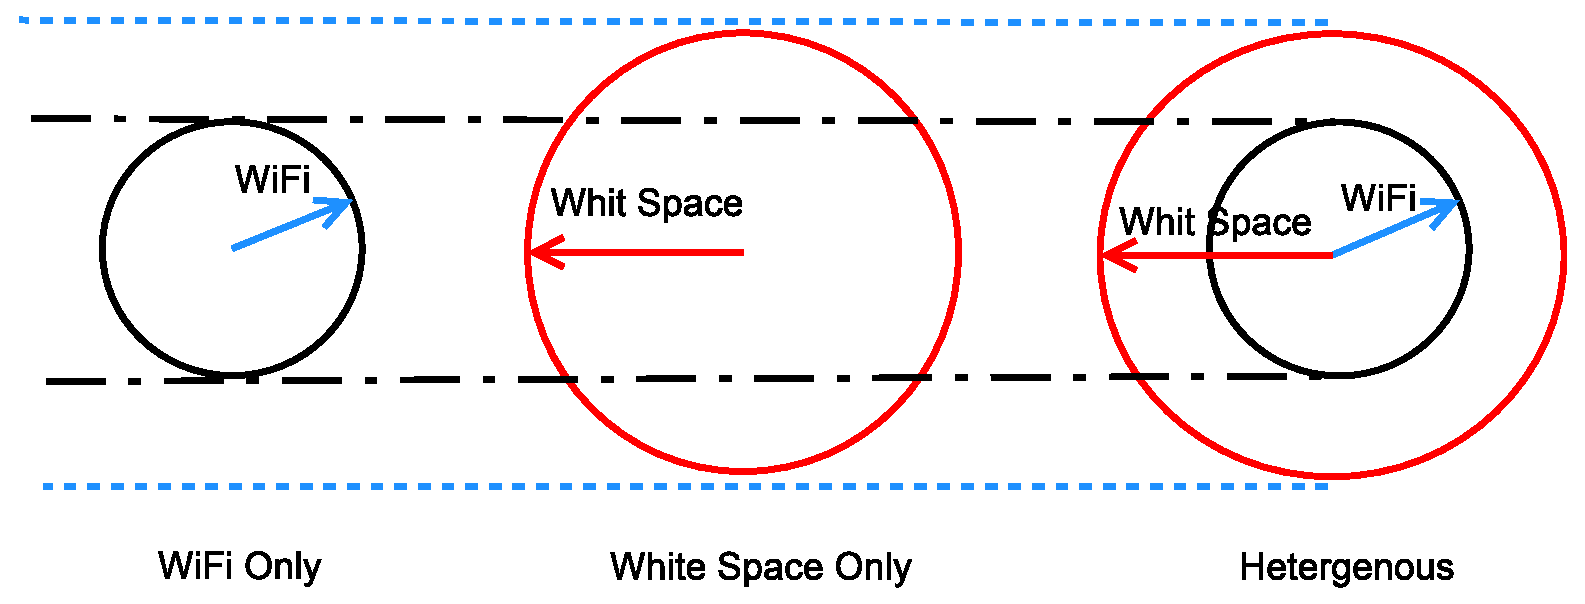
\includegraphics[width=84mm]{figures/lowtraffic}
\vspace{-0.1in}
\caption{Low Traffic Scenario}                                                                 
\label{fig:lowtraffic}
%\vspace{-0.1in}
%\end{figure}

%\begin{figure}[H]
%\vspace{-0.0in}
%\centering
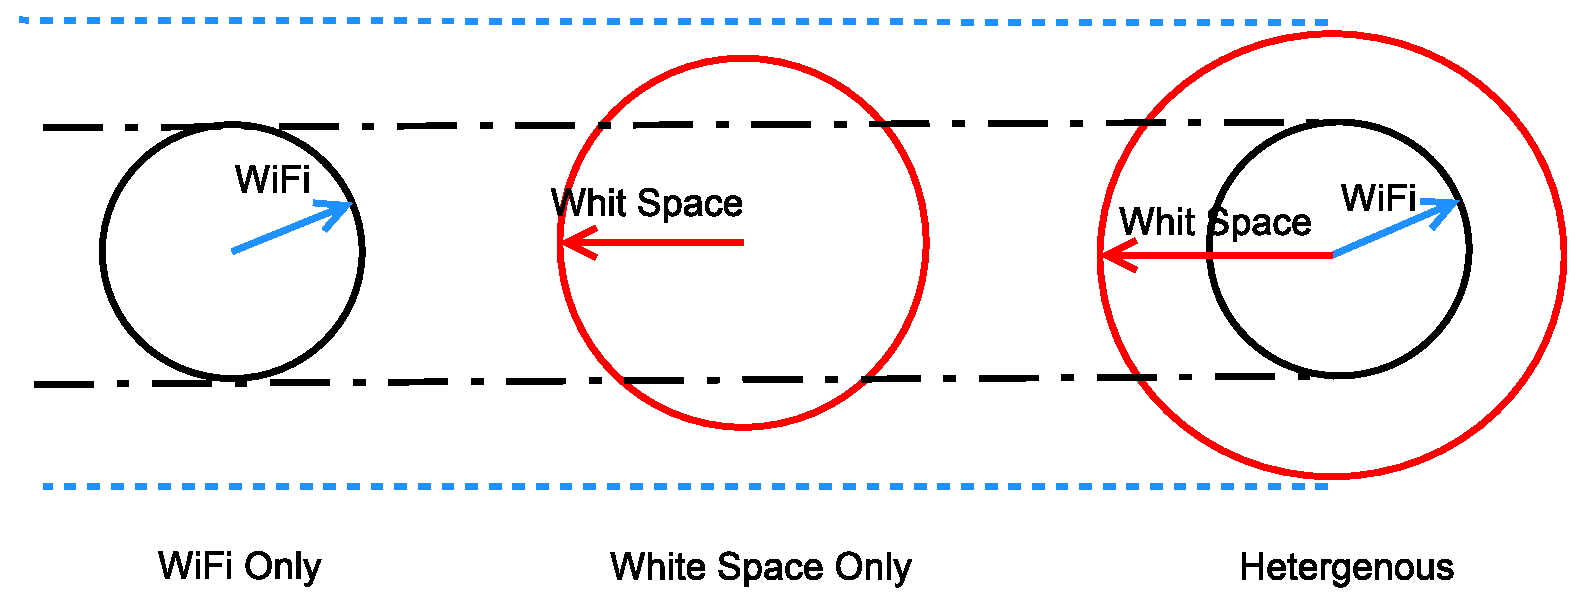
\includegraphics[width=84mm]{figures/mediumtraffic}
\vspace{-0.1in}
\caption{Medium Traffic Scenario}                                                                 
\label{fig:mediumtraffic}
%\vspace{-0.1in}
%\end{figure}


%\begin{figure}[H]
%\vspace{-0.0in}
%\centering
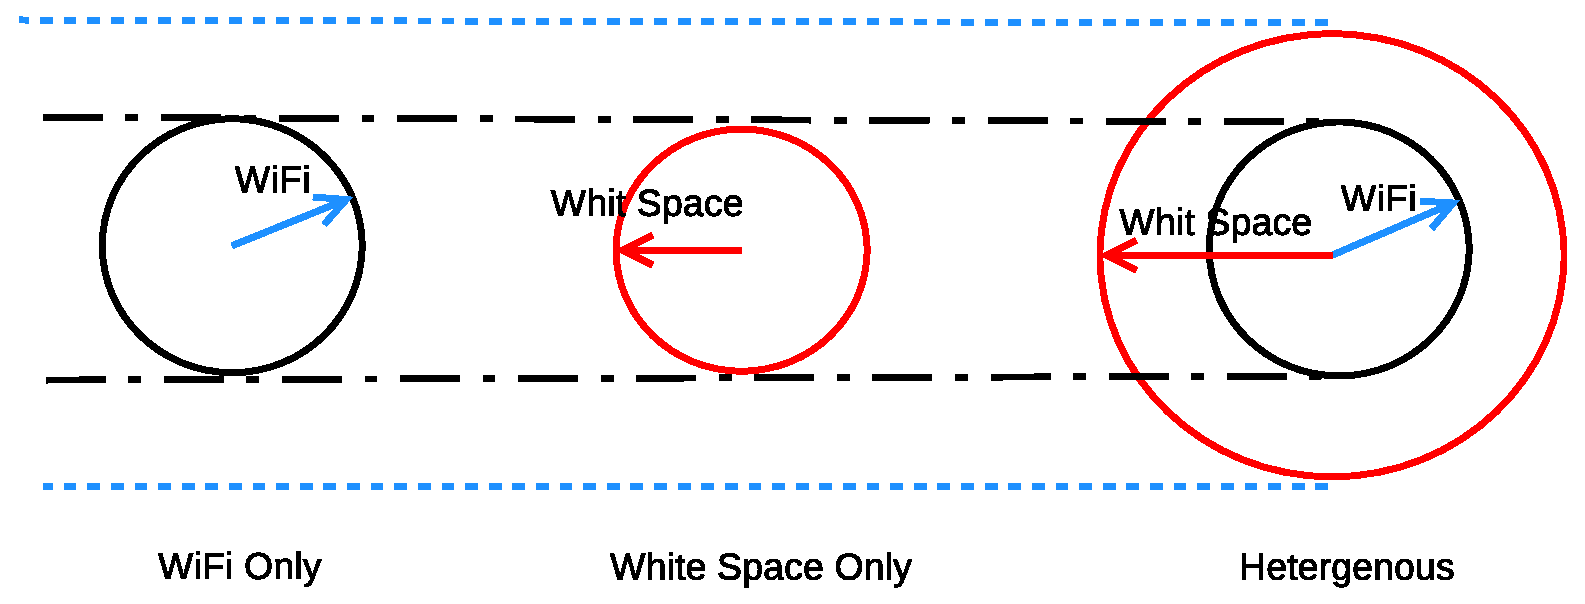
\includegraphics[width=84mm]{figures/hightraffic}
\vspace{-0.1in}
\caption{High Traffic Scenario}                                                                 
\label{fig:hightraffic}
\vspace{-0.1in}
\end{figure}

% Relaxed linear program
Given a target area $G$ with the traffic demand distribution $\gamma$, the service area 
of all kinds access points $S_t$, and the coverage rate $p$, the capacity of access point $C_t$ could 
be calculated based on the number of radios, Friis model in Eq.~\ref{eq:friis} and restriction constraints in Eq.~\ref{eq:servicearea}
or from in-field measurement~\cite{cuileveraging}. 
When the target area is served, the reward of the area 
could be calculated as $R$. However, the reward of service carrier does not influence the 
optimal deployment since the total reward is a constant when the user number is constant in the 
service area in our scenario. Furthermore, the minimum number of access points could be found through 
a relaxed linear program as follows. 

\noindent
{\bf Sets:}
\begin{tabular}{ll}
$B$ & Set of Bands \\
$T$ & Type of Access Point\\
\end{tabular}

\noindent
{\bf Parameters:}\\
\\
%\vspace{0.1in}
%\begin{tabular}{lll}
\begin{tabular}{llp{3.4cm}}
$G$ &  & Target Area\\
$\gamma$ & & Traffic Demand Distribution\\
$p$ & & Coverage Rate\\
$S_t$ & $t \in T$ & Coverage Area of Type t AP\\
$O_{b,t}$ & $b \in B, t \in T\ binary$ & Channel Occupied by Type t AP\\
$N_b$ & $b \in B\ $ & Available channel of a band in Target Area\\
$C_t$ & $t \in T$ & Channel capacity of Type t AP\\
\end{tabular}


\noindent
%\vspace{2pt}
{\bf Variables:}\\
\\
%\vspace{1pt}
\begin{tabular}{llr}
$a_t\ge0$ & $t \in T$ & Number of Type t AP\\ 
\end{tabular}

\noindent
{\bf Objective:}
\begin{align}
& Min \sum_t a_t
\end{align}

\noindent
%{\bf Constraints:}
{\bf Coverage Constraint:}
\begin{align}
\label{opt:coverage}
\sum_t a_t\cdot S_t \ge G*p
\end{align}
\noindent
{\bf Capacity Constraint:} 
\begin{align}
\label{opt:capacity}
\sum_t a_t\cdot C_t \ge G\cdot \gamma
\end{align}
\noindent
{\bf Resource Constraint:} 
\begin{align}
\label{opt:resource}
\sum_t a_t\cdot O_{b,t} \le N_b
\end{align}

{\bf Spatial Constraint:} 
\begin{align}
\label{opt:resource}
a_t < \frac{G}{S_t}\cdot\frac{2}{3}\cdot N_b
\end{align}


The linear program relaxes the coverage constraint without providing a key parameter
where the access points are located. Moreover, the linear program may provide 
multiple results since different types of access points could have the same service area, 
(e.g. in a low traffic demand case) The result of the linear program is the lower bound
on the number of access points. 

In order to find a practical access points deployment in multiband scenario, we represent 
a greedy local search algorithm in Alg.~\ref{alg:gls}. The service area of access points varies 
across diverse population distributions. Assume the cost of building an access point is the same as $C_a$. 
When an access point is built, the more service area the better. Thus, heterogeneous access points
could always have better performance. However, since there are a limited spectrum resources,
we have to balance the usability of heterogeneous access points which reduce the cost of building 
a network, and single radio access point which may cover more area.

In the linear program, the reward $R$ is a constant of the area $G$. But for a single heterogeneous access
point deployment, we have to compare its reward and cost to separately using the radios.
In a certain area, a heterogeneous AP has radius $r_1$. If we separately use the radios with
radius $r_2,r_3,\dots r_n$, the reward is uniformly distributed and the heterogeneous reward is defined as:

\begin{equation}
\label{eq:unitprice}
H_r=(n-1) C_a - \frac{R}{G}\cdot\sum f_s(r_n)
\end{equation}

Here, $f_s(r)$ is the area calculated function, for example, $f_s = \frac{3\sqrt{3}}{2}r^2$ when a 
hexagonal coverage model is applied. In the framework, the access point type with greater reward 
is going to deployed first until the available resources are used up. When two types of access points
share the same unit price, considering the spatial reuse, the access points with high frequency channels
will be chosen. The deployment starts from the edge of the given plane and we use a protocol model
to find the available access point types. If the combination of a unit 
grid could be covered by an access point, we put the unit grid in the coverage area until the access
point can not access any more of grid. Then we switch to another available access point. The process is like
a Teris game, when a given access point is filled, it will be deleted.
% Algorithm for lower bound approaching
\begin{algorithm}
\caption{Multiband Heterogeneous AP Deployment}
\label{alg:gls}
\begin{algorithmic}[1]
\REQUIRE  ~~\\
$G$: Target Area \\
$R$: Reward of Target Area \\
$\gamma$: Traffic Demand Distribution\\
$p$: Coverage Rate\\
$S_t$: Coverage Area of Type t AP \\
$O_{b,t}$: Channel Occupied by t Type AP\\
$N_b$: Available channels of a Band in Target Area\\
$C_t$: Channel Capacity of Type t AP
\WHILE {$\sum A\cdot S_t < p$}
\STATE Rank available AP type according to their unit price $H_r$
\STATE Rank available AP type according to radio numbers
\IF {The reminder area $G_r$ is larger than all the available AP}
\STATE Choose the AP has the largest coverage area $S_t$
\ELSE 
\STATE Find the available AP type whose coverage area $S_t=min{S_t>G_r}$
\ENDIF
\STATE Deploy an AP at the left up edge of un-covered area
\STATE Fill the AP with one neighbor unit grid and move the AP in the center of the coverage area
\STATE Update Channel Resource $O_{b,t}, N_b$
\STATE Update Output Access Point $A$
\ENDWHILE
\ENSURE ~~\\
The number of Access Points and Deployment\\
\end{algorithmic}
\end{algorithm}
% Algorithm analysis and justify

Generally, we employ access points with larger coverage capacity to fill in the area. Then 
through the algorithm, we could cover the target area by the most efficient access point type,
step by step until a  minimum number of access points and a practical multiband wireless deployment is achieved.

\section{Data Process}
\label{sec:experiment}
In this section, we show the results of the experiments and analyze the results of our framework. Different metric are involved to evaluate the framework.

\emph{Accuracy in Signal Level} is the percents of predict signal level in the measured signal level interregional. We evaluate both the theoretic results from path loss equation and the context-aware base framework in this scenario.

\emph{Performance Improvement} is the percents of throughput of multi-band over single band.


\subsubsection{Indoor Experiments} 
We first use the signal level of test data in different band to calculate the signal level of different bands. Then we use the signal level database to predict the signal level. The results from the two methods are compared with the measured signal. The graph shows the calculation results, the context-aware results for fixme set of training data, and the measured results.

%fixme graph of calculation, context-aware and measured

The amount of information in context-aware database will influence the accuracy of results. How much information is enough for the prediction for the signal is an interesting question. We put the same test data into different size context-aware database to produce the output signal level in different bands. The graph shows the signal level prediction in different context-aware database and the measured results.

%fixme graph of context-aware signal in different loops, different loops in different curves

Following graph shows the \emph{Accuracy in Signal Level} for different size context-aware database in indoor experiments.

% fixme hint graph of accuracy in signal level


Through the multi-band framework, we analyze the influence of time window for the performance estimation. We show the estimation in different size of time window and the measured throughput.

%fixme estimation of different time window and measured throughput


If we implement the band switching, the improvement is shown in the following graph,

%fixme multi-band improvement













%fixme could we show some results only rely on emulator data??? such as the signal level prediction? show in the ideal channel state, the pathloss equation calculation make more sense???????????????????????????????????






\subsubsection{In-field Experiments} 
In the previous section, we analyze and shows the results of indoor experiments. In this section, we will introduce the results of in-field experiments.
We also has the same metric as in-door experiments for evaluation. 
The graph shows the calculation results, the context-aware results for fixme set of training data, and the measured results.

%fixme graph of calculation, context-aware and measured

In in-field status, there are more factors will influence the signal level. We analyze the influence of information amount for context-aware database in in-field situation and shows in the following graph.

%fixme graph of context-aware signal in different loops, time/number as x-axis

Following graph shows the \emph{Accuracy in Signal Level} for different size context-aware database in in-field experiments.

% fixme hint graph of accuracy in signal level


Through the multi-band framework, we analyze the influence of time window for the performance estimation. We show the estimation in different size of time window and the measured throughput.

%fixme estimation of different time window and measured throughput



The potential improvement is shown in the following graph,

%fixme improvement for multiband switich

























%Detail may not useful
%Parsing script
%In our experiments, we are constantly collecting large amounts of data, including the received signal level, current location, velocity, and time of day. Working with the memory-limited Gateworks boards, it became necessary to implement a solution to collect large amounts of data without exhausting the available memory space on the boards. Thus, we compiled a script to parse an undetermined number of data files containing the raw data collected from the ongoing experiments. Utilizing the Perl programming language, which the Gateworks boards are capable of running, the script scans every file in a directory we specify and parses them, looking specifically for signal level, lat/long location, velocity, and time data recorded from the experiments. Upon finding this information, the script reformats the data by placing it into a .csv file. Additionally, using the location data, the script calculates the  distance between the transmitting and receiving boards and adds this information to the .csv file. Upon parsing the data, the raw experimental data files can simply be delete from memory, freeing up space for the data of subsequent experiments.

%Activity monitor script
%For in-situ experiments, the need became apparent to track the number of new incoming packets and compare it with the number of previously received packets. Additionally, this needed to be done for each of the four wireless radios on the board. In doing this, we identify the most efficient frequency band to transmit data. To implement this system, a script was needed to run efficiently in the background while experiments were taking place. To achieve this, we wrote a bash shell script to run directly on the board without relying on any higher level programming language that could potentially cause greater performance overhead. As a result, the script only consumes one to two percent of CPU resource. The script begins by examining the received bytes across each radio for a length of 30 seconds and placing the bytes received each second on a new line in a file. Upon the completion of the 30 second buffering time period, the next second of received bytes on each radio is read and compared with the last 30 seconds of received data. This ratio of the most recent received data to old received data is then calculated and written to four files, one for each radio, for its subsequent use in selecting which radio to transmit/receive from.


\section{Related Work}
\label{sec:related}
%%fixme add the daparowrds
%The conventional definition of the spectrum opportunity, which is often defined as "A band of frequencies that are not being used by the primary user of that band at a particular time in a particular geographic area."\cite{kolodzy2001next}


Elecronmagnetic radio spectrum is a natural resource licensed by governments.  the Federal Communications Commission(FCC) published a report prepared by the Spectrum-Policy Task Force, discussed improving the way to manage this resource in the United States \cite{federal2002spectrum}. 

The limited resource make people find new ways to improve the effciency of the frquency resource utility. There are two methods to arrive this target. First is the underlay approach, constraints on the transmission power of second users. Second is the overlay approach, identify and exploit spatial and temporal spectrum white space by second users \cite{zhao2007survey}.
The first approaching require more support from the hardware, the second approaching can be achieved by soft-ware radios only. The frequency is not occupacied all the time in all the regions.


%ways to improve the frequency efficient



The underutilization of the electromagnetic spectrum leads to a definition of \emph{Spectrum Opportunity} as a band of frequencies assigned to a primary user, but at a particular time and specific geographic location, the band is not being utilized by that user \cite{kolodzy2001next}.



%Cognitive Radio

%fixme FCC definition
%The definition adopted by Federal Communications Commission(FCC):"Cognitive radio: A radio or system that senses its operational electromagnetic environment and can dynamically and autonomously adjust its radio operating parameters to modify system operation, such as maximize throughput, mitigate interference, facilitate interoperability, access secondary markets."
The concept of \emph{Cognitive Radio} is introduced as a novel approach for improving the utilization of the wireless spectrum and the tasks for cognitive radio is summarized in \cite{haykin2005cognitive}. The three on-line cognitive tasks include: \emph{Radio-scene analysis, Channel identification, Transmit-power control and dynamic spectrum management} \cite{haykin2005cognitive}.
Underutilized terrestrial TV bands will be able to be used by wireless communication. Combine different bands to create Multi-bands/Multi-channels system is a new field of \emph{Cognitive Radio} to improve the performance of wireless systems in different
environments(e.g., as in ~\cite{MOAR}). 

%Multi-channel
A bunch of work has been done on \emph{Radio-scene analysis} and \emph{Channel identification} dating back to Simon Haykin \cite{haykin2005cognitive}.
Some work of Multi-bands/Multi-channels in
cognitive radios focus on optimize performance, such as avoiding frequency diversity \cite{rahul2009frequency}. 
In \cite{OAR} an opportunistic algorithm is intorduced to balance the cost of \emph{spectrum sensing, Channel switching} and the gain of these activities.
%fixme, add more multichannel and add pathloss exponent

%spectrum sensing

One of the most important components of the congnitive radio concept is the ability to measure, sense, learn and be aware of the parameters related to the radio channel characteristics, availability of spectrum and power, radios operating envrionment \cite{yucek2009survey}. Spectrum sensing becomes the most important component for the estabilishment of congnitive radio. \cite{yucek2009survey}. 





%Adaptation algorithms
There is a lot of recent research on the design of adaptation algorithms, both rate adaptation and \emph{band/channel} adptation of cognitive radio systems. These researches are focusing on the \emph{Spectrum sensing and Channel switching strategies}.

\textbf{Evaluation of Channel Conditions}. Channel condition is the most important component of adaptation. 
There are two classes of rate adaptation mechanisms that have been developed. 
These mechanisms are focused on rate adaptation. The first generation adaptation algorithms are loss-triggered. The adaptation algorithm based on the statistics of a previous period of transmission. 
Second generation rate adaptation schemes diagnose the cause of a loss and appropriately adjust the data rate \cite{biaz2008rate, camp2010modulation}, such as a SNR-triggered protocol. 
Our work consider both the statistics information of the previous transmission and the dynamic information in context-aware based channel qualification.

\textbf{Evaluation of Adaptation}. Most of the prior work of rate adaptation protocols has investigated the effectiveness via throughput comparison \cite{camp2010modulation}. This is the metric we also employ in the paper to evaluate the performance. Furthermore, we also evaluate the amount of context-aware information in prediction.
 
\textbf{Primary Second User}. Some other works focus on Multi-channel which bandwidth range limits in 2.4GHz \cite{MOAR} or in a continuous bandwidth considering frequency diversity \cite{rahul2009frequency}. 
Significant research on the design of channel selection algorithms has been done \cite{radunovic2011dynamic,raniwala2005architecture}. Algorithms are generated for second user to distinguish whether the channel is free or in less utility state as soon as possible \cite{cordeiro2007c}. These works indicate the way to employ limit frequency work in high efficiency. In contrast, we are trying to improve the wireless performance taking more frequency bands.

Our work is motivated by prospective white band using for TV today and exploit the comparison across all the avaiable bands in the future. It is a kind of extention of multi-channel adaptation. Our approach classifies the performance based upon combination of in-field measurents and ideal channel conditions on \emph{channel emulator}. Most of the research focus on the stopping rules of spectrum sensing \cite{sabharwal2007opportunistic, OAR}. In contrast, we use the data and framework to classify the performance across different bands based on the parameters we get from the context-aware information.
{\bf .} 


\section{Conclusion}
\label{sec:conclusion}
In this paper, we jointly considered the use of WiFi and white space bands for 
%deploying wireless access networks across a broad range of population densities.
%To consider network deployment costs, we proposed a Multiband Access Point Estimation 
%framework to find the number of access points required in a given region.
%We then performed spectrum utilization measurements in the DFW metropolitan 
%and surrounding areas to drive our framework and find the influence of white spaces on
%network costs in these representative areas. Through 
%extensive analysis across varying population density and channel combinations across bands, 
%we show that white space bands can reduce the number of access points by 1650\%
%and 660\% in rural and sparse urban areas, respectively. However, the same cost savings
%are not achieved in dense urban and downtown type area. Finally, we investigate different 
%band combinations in two population densities to show that greater access to white space 
%channels have greater total savings of mesh nodes when the total number of channels used 
%in the network is fixed (i.e., given a total number of allowable WiFi and white space channels). 
%As the population and spectrum utilization increase, the cost savings of white space bands
%diminish to the point that WiFi-only channel combinations can be optimal.




%\chapter{Spectrum Adapatation in Backhual Tier Network} 
\label{ch:wm}


%\section{Hetergeneous Access Point Band Selection}
%\label{sec:moa_problemformulation}
%
%% Introduce the content of this section
%In this section, we illustrate the challenges of hetergenous access point 
%band selection in wireless network deployment and formulate the problem of band 
%selection in mesh network deployments jointly using WiFi and white space bands. 
%Further, we present a linear program and MHAPD(Multiband Hetergeneous AP Deployment) algorithm for estimating the 
%access point number to serve the traffic demand of a given population.
%Then we discuss the application of the algorithm in uniform population
%distribution and non-uniform population distribution with spectrum resource 
%variation to tell the general rules in picking up channels for access points.
 
%\subsection{White Space Opportunity and Challenge}
%\label{subsec:motivation}

%% Propagation
%Wireless propagation is the behavior of the signal loss characteristics 
%when wireless signals are transmitted through the wireless medium.
%The strength of the received signal depends on both the line-of-sight
%path (or lack thereof) and multiple other paths that result from 
%reflection, diffraction, and scattering from 
%obstacles~\cite{andersen1995propagation}. The widely-used Friis
%equation characterizes the received signal power $P_r$ in terms 
%of transmit power $P_t$, transmitter gain $G_t$, receiver gain $G_r$, 
%wavelength $\lambda$ of the carrier frequency, 
%distance $R$ from transmitter to receiver, and path loss exponent 
%$n$ according to~\cite{friis}:
%\begin{equation}
%\label{eq:friis}
%P_r=P_t+G_t+G_r+10n \log_{10}\left( \frac{\lambda}{4\pi R}\right)
%\end{equation}
%Here, $n$ varies according to the aforementioned environmental 
%factors with the value of two to five in typical outdoor 
%settings~\cite{rappaport}.

% Hetergenous access points
%Despite sufficient levels of received signal, interference can cause channels
%to be unusable (e.g., due to high levels of packet loss) or unavailable (e.g.,
%due to primary users in cognitive radios~\cite{haykin2005cognitive}).
%Prior work has worked to reduce cost through gateway deployment, channel 
%assignment, and routing~\cite{he2008optimizing,tang2005interference}.
%Most of existing works try to reduce the intra-network interference or increase
%the channel usability level of wireless network deployment
%~\cite{si2010overview,joshi2009efficient}. However, the access point service area
%variation becomes an important problem when considering the availability of white space bands.  
%Jointly considering the propagation and single channel capacity, the access points 
%with different configuration (e.g. radios) in the same area, or with same configuration 
%in diverse population density areas (e.g. downtown, rural) could have different service ranges.
%
%% Explain multiband and hetergenous access points
%When wireless devices operate in WiFi bands, the channel separation is relatively
%small (e.g., 22 MHz for the 2.4 GHz band). As a result, many works assume that
%the propagation characteristics across channels are similar. However, with the
%large frequency gaps of WiFi and white space bands (e.g., several GHz),
%propagation becomes a key factor in the deployment of wireless networks with both bands.
%Here, a frequency band is defined as a group of channels which have
%small separation meaning similar propagation characteristics.
%In this work, we consider the diverse propagation and activity characteristics
%for four total frequency bands: 450 MHz, 800 MHz, 2.4 GHz, and 5.2 GHz.
%We refer to the two former frequency bands as white space bands and
%the two latter frequency bands as WiFi bands.
%A general way to increase the capacity of a single access point is to add channels
%through radios~\cite{raniwala2005architecture}. The assumption all the channels have
%the same propagation does not fit for WiFi and white space hetergenous scenario.
%When a white space band channel added to an access point, the capacity and service 
%range could increase simultaneously. The differences in propagation and constraints 
%of network deployment create opportunity for the joint use of white space and 
%WiFi bands in wireless access networks according to the environmental characteristics 
%(e.g., urban or rural and downtown or residential) of the deployment location.
%
%% Network Constraints
%Typically, the deployment of wireless access networks is subject to coverage and capacity
%constraints for a given region. Coverage is defined with respect to the ability of
%clients to connect to access points within their service area.  We use a coverage
%constraint ratio of $95\%$ in this work for a target area~\cite{robinson2010deploying}.
%Capacity is defined with respect to the ability of a network to serve the traffic 
%demand of clients.  Spatial reuse allows improved capacity, but increases the cost
%of deploying a network by increasing the total number of access points required.
%Hence, for densely populated areas the greatest level of spatial reuse possible
%is often desired. And the deployment cost could be significant reduced through access 
%points with high capacity with more centralized using radios. In contrast, 
%sparsely-populated rural areas have lower traffic demand per unit area. Thus, 
%aggregating this demand with lower-frequency, white space bands could be highly 
%effective in reducing the total number of access points required to achieve 
%similar coverage and capacity constraints. Moreover, since less TV channels tend
% to be occupied in sparsely populated areas~\cite{msdatabase}, a larger number 
% of white space bands can be leveraged in these areas. 

% More variation in population distribution



\section{Heterogeneous Access Point Band Selection}
\label{subsec:moaproblem}

% Assumptions of the network
As opposed to previous works such as
~\cite{franklin2007node,robinson2010deploying,si2010overview}, 
these works focus on heterogeneous access point selection 
for wireless access networks which jointly employ WiFi and white space bands.
We propose a relaxed linear program to find the lower bound of the number of access points
and MHAPD algorithm  to approach the lower bound number of access points which serve
the traffic demand of a certain area. We assume the service provider has a limited number 
of spectrum resources and radios have similar configurations in terms of transmission power and bandwidth per 
channel use. Each radio on an access 
point operates with a classic protocol model as introduced in~\cite{gupta2000capacity}. 
We further assume that there is a given take rate and traffic demand for a given 
population (as specified in Section~\ref{sec:moaexperimentdesign}).

%% Capacity constraint
%A network deployment should ideally provide network capacity equal to the demand of the service 
%area to maintain the capacity constraint. The demand of a service area could be calculated as the 
%summation of individual demands all over the service area $D_a=\sum_{p\in P}D_p$. Since 
%household demand for Internet has been previously characterized~\cite{rosston2011household}, 
%$D_a$ could represent the population distribution $f$ and service area $k$ as 
%$D_a=\sum_{f \in F,k \in K}\bar{D_p}*f*k$. 
%The capacity constraint could be represented with access points set $M$ according to:
%\begin{equation}
%\label{eq:nlbound}
%\sum_{m \in M}C_r^m \ge \sum_{f \in F,k \in K}\bar{D_p}*f*k
%\end{equation}
%% Coverage constraint
%At the same time, the wireless network must additionally satisfy the coverage constraint in the service 
%area where the access points provide connectivity for client devices. 
%Generally, a coverage of $95\%$ is acceptable for wireless access networks~\cite{robinson2010deploying}.
%The object of this work is to find the best possible number of access points so that the network has good 
%connectivity and enough capacity to satisfy the traffic demands.


% Hetergeneous Access point & resource constraint
Under the capacity and coverage constraints, the service area of a heterogeneous multiband access point deployments
varies according to the traffic demand. The service area is limited by the propagation range when the traffic 
demand is low  when the traffic demand is high, the service area is limited by the radio capacity.
The radius of the service area $r_s$ could be represented as:
\begin{equation}
\label{eq:servicearea}
r_s=min\{r_p,r_c\}
\end{equation}
Here, $r_p$ represents the propagation range of a radio in the access point, and $r_c$ is the capacity range of 
a a radio in the access point. When the traffic demand is distributed uniformly in a circle, from 
Eq.~\ref{eq:nlbound} the capacity range $r_c$ could be noted as $r_c=\sqrt{k/\pi}$. Moreover,
the propagation range and capacity range could be determined by the environment, traffic distribution, and
transmission power control~\cite{robinson2010deploying}. These factors are out of the scope of this work, but they could
easily be added to the model for calculation of the heterogeneous access point service area. To simplify the 
problem and focus on the role of multiple frequency bands, we assume the traffic demand is uniformly distributed and the propagation 
follows Friis rule as Eq.~\ref{eq:friis}. When the target area is given, we could obtain the service area of
each access point type through~\ref{eq:servicearea}, we then adjust the transmit power of each radio
to reduce the interference.

% Variation of radios
When the traffic demand of an area is constant, the service area of a heterogeneous access point 
varies with the radios due to the constraints. We assume all the access points have the same number of radios and channel 
resources.
% Lower traffic demand case
In a low traffic demand scenario, the service radius reaches the radio propagation range.
A high frequency WiFi radio will have a smaller service area since the signal attenuate faster; while the white
space radio could have a larger service area due to the longer propagation range; and a heterogeneous access point who has
both WiFi radios and white space radios has the same range of as low frequency radios access point. An example is
shown in Fig.~\ref{fig:lowtraffic}.
% Medium traffic demand case
In a medium traffic demand scenario, heterogeneous access points and white space access points will 
have the same size service area which is larger than high frequency WiFi only access points as shown in Fig.
~\ref{fig:mediumtraffic}.
% High traffic demand case
With high traffic demand, all access points will have the same service area due to capacity constraint 
as shown in Fig.~\ref{fig:hightraffic}. White space bands could reduce the cost of wireless network 
deployment due to greater inter node spacing. 
Thus, lowest cost for covering a certain area is to use white space bands in all access points 
it the traffic demand and user density is sufficient. 
%based on the analysis.
However, spectrum resources are limited and the use of white space bands 
are restricted in major cities in the US due to TV channel occupancy~\cite{msdatabase}. 
% Problem
Thus, the tradeoff between centralized use of  white space bands or mixed use of white space
bands and WiFi bands under multiple traffic demands is question for wireless network deployment. The problem
could be modeled as how to use the minimum number of different sizes of service area according to 
radio combinations to cover a certain 2- D plane. This problem is a to deploy different size of cells in 
a given plane, which is a NP-hard bin packing problem~\cite{martello1998exact}. We propose a relaxed 
linear program to achieve the lower bound of the number of access points and a heuristic algorithm to 
approach the lower bound.



\begin{figure}
%\vspace{-0.0in}
\centering
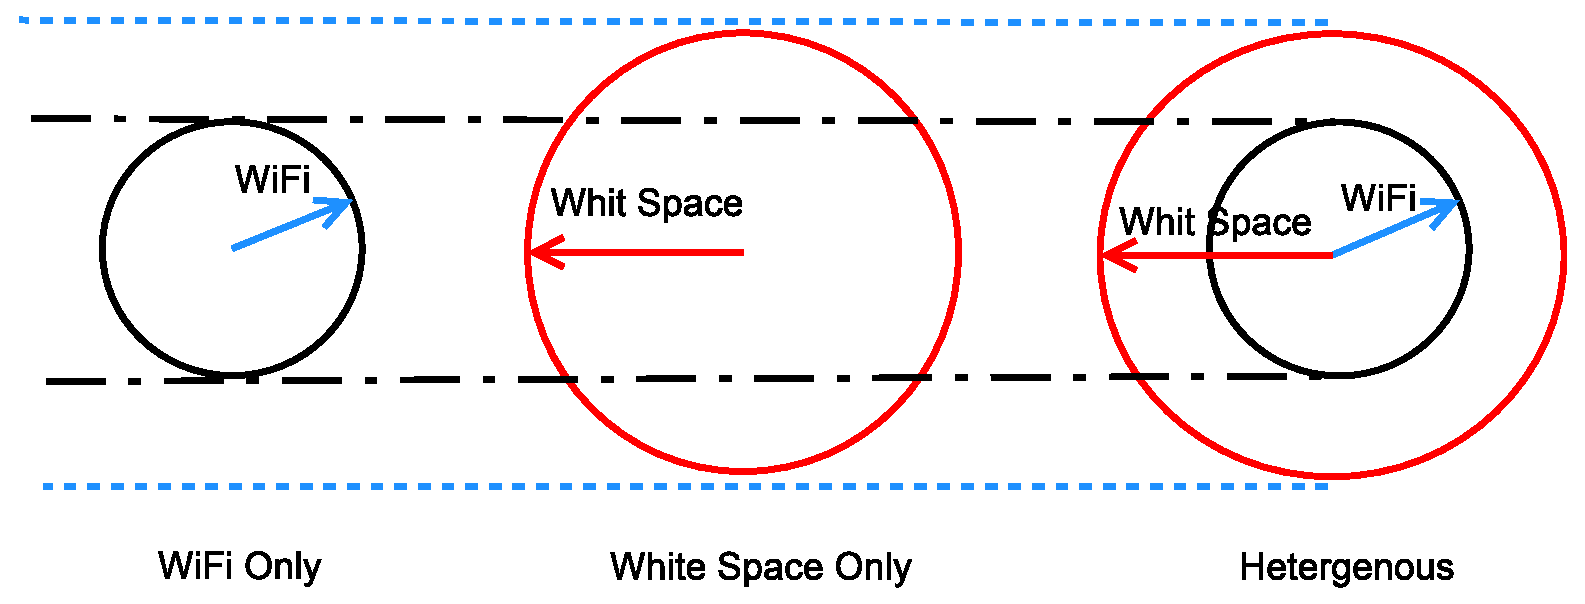
\includegraphics[width=84mm]{figures/lowtraffic}
\vspace{-0.1in}
\caption{Low Traffic Scenario}                                                                 
\label{fig:lowtraffic}
%\vspace{-0.1in}
%\end{figure}

%\begin{figure}[H]
%\vspace{-0.0in}
%\centering
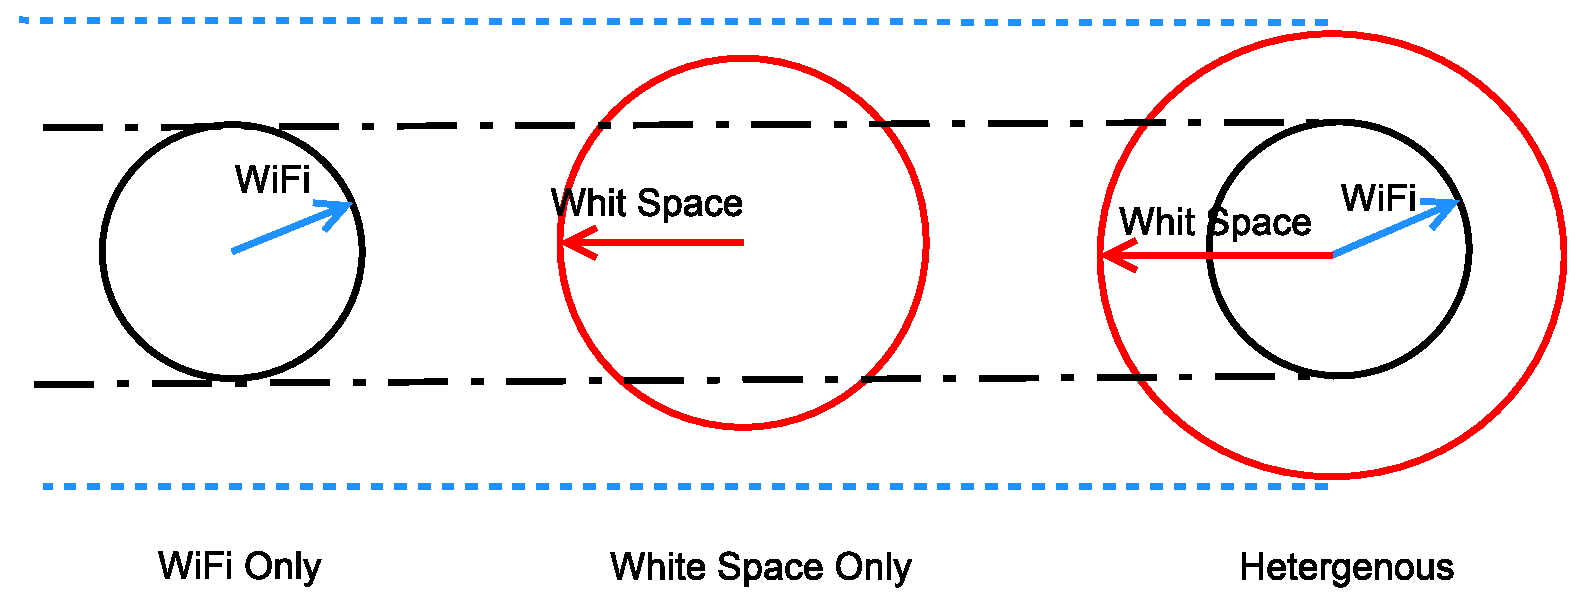
\includegraphics[width=84mm]{figures/mediumtraffic}
\vspace{-0.1in}
\caption{Medium Traffic Scenario}                                                                 
\label{fig:mediumtraffic}
%\vspace{-0.1in}
%\end{figure}


%\begin{figure}[H]
%\vspace{-0.0in}
%\centering
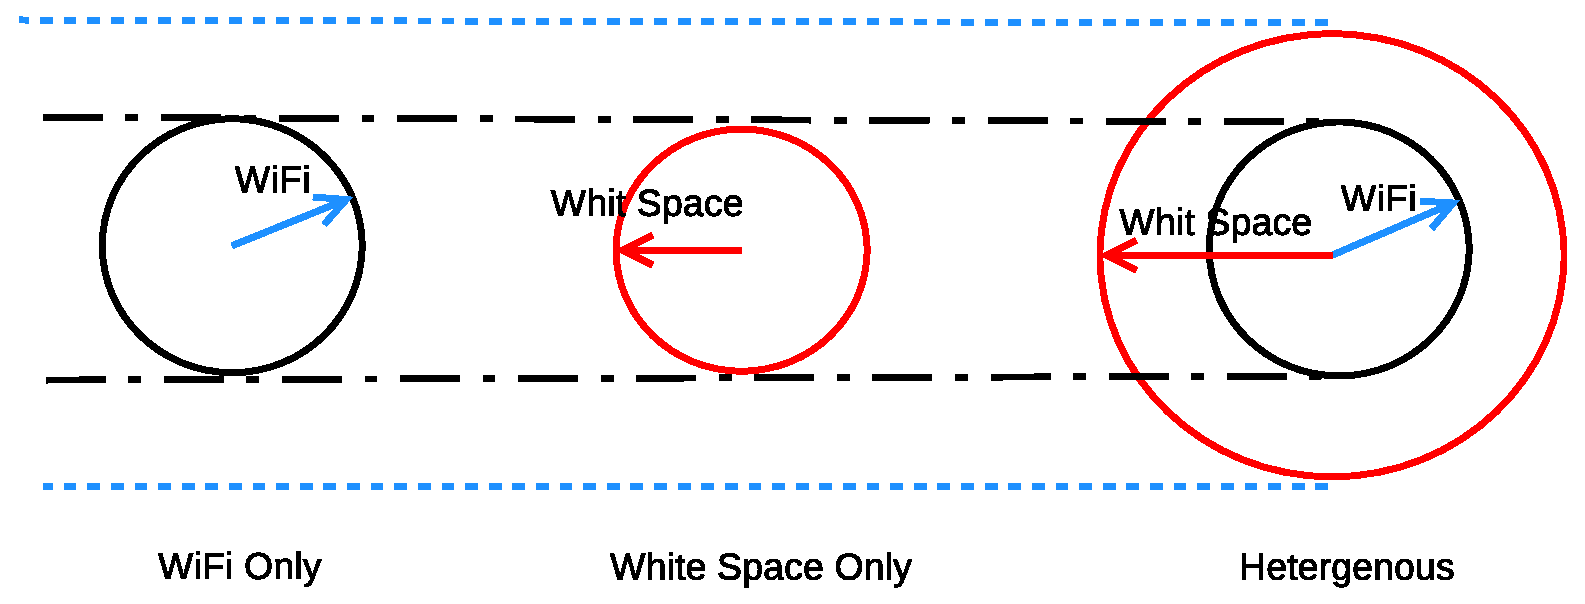
\includegraphics[width=84mm]{figures/hightraffic}
\vspace{-0.1in}
\caption{High Traffic Scenario}                                                                 
\label{fig:hightraffic}
\vspace{-0.1in}
\end{figure}

% Relaxed linear program
Given a target area $G$ with the traffic demand distribution $\gamma$, the service area 
of all kinds access points $S_t$, and the coverage rate $p$, the capacity of access point $C_t$ could 
be calculated based on the number of radios, Friis model in Eq.~\ref{eq:friis} and restriction constraints in Eq.~\ref{eq:servicearea}
or from in-field measurement~\cite{cuileveraging}. 
When the target area is served, the reward of the area 
could be calculated as $R$. However, the reward of service carrier does not influence the 
optimal deployment since the total reward is a constant when the user number is constant in the 
service area in our scenario. Furthermore, the minimum number of access points could be found through 
a relaxed linear program as follows. 

\noindent
{\bf Sets:}
\begin{tabular}{ll}
$B$ & Set of Bands \\
$T$ & Type of Access Point\\
\end{tabular}

\noindent
{\bf Parameters:}\\
\\
%\vspace{0.1in}
%\begin{tabular}{lll}
\begin{tabular}{llp{3.4cm}}
$G$ &  & Target Area\\
$\gamma$ & & Traffic Demand Distribution\\
$p$ & & Coverage Rate\\
$S_t$ & $t \in T$ & Coverage Area of Type t AP\\
$O_{b,t}$ & $b \in B, t \in T\ binary$ & Channel Occupied by Type t AP\\
$N_b$ & $b \in B\ $ & Available channel of a band in Target Area\\
$C_t$ & $t \in T$ & Channel capacity of Type t AP\\
\end{tabular}


\noindent
%\vspace{2pt}
{\bf Variables:}\\
\\
%\vspace{1pt}
\begin{tabular}{llr}
$a_t\ge0$ & $t \in T$ & Number of Type t AP\\ 
\end{tabular}

\noindent
{\bf Objective:}
\begin{align}
& Min \sum_t a_t
\end{align}

\noindent
%{\bf Constraints:}
{\bf Coverage Constraint:}
\begin{align}
\label{opt:coverage}
\sum_t a_t\cdot S_t \ge G*p
\end{align}
\noindent
{\bf Capacity Constraint:} 
\begin{align}
\label{opt:capacity}
\sum_t a_t\cdot C_t \ge G\cdot \gamma
\end{align}
\noindent
{\bf Resource Constraint:} 
\begin{align}
\label{opt:resource}
\sum_t a_t\cdot O_{b,t} \le N_b
\end{align}

{\bf Spatial Constraint:} 
\begin{align}
\label{opt:resource}
a_t < \frac{G}{S_t}\cdot\frac{2}{3}\cdot N_b
\end{align}


The linear program relaxes the coverage constraint without providing a key parameter
where the access points are located. Moreover, the linear program may provide 
multiple results since different types of access points could have the same service area, 
(e.g. in a low traffic demand case) The result of the linear program is the lower bound
on the number of access points. 

In order to find a practical access points deployment in multiband scenario, we represent 
a greedy local search algorithm in Alg.~\ref{alg:gls}. The service area of access points varies 
across diverse population distributions. Assume the cost of building an access point is the same as $C_a$. 
When an access point is built, the more service area the better. Thus, heterogeneous access points
could always have better performance. However, since there are a limited spectrum resources,
we have to balance the usability of heterogeneous access points which reduce the cost of building 
a network, and single radio access point which may cover more area.

In the linear program, the reward $R$ is a constant of the area $G$. But for a single heterogeneous access
point deployment, we have to compare its reward and cost to separately using the radios.
In a certain area, a heterogeneous AP has radius $r_1$. If we separately use the radios with
radius $r_2,r_3,\dots r_n$, the reward is uniformly distributed and the heterogeneous reward is defined as:

\begin{equation}
\label{eq:unitprice}
H_r=(n-1) C_a - \frac{R}{G}\cdot\sum f_s(r_n)
\end{equation}

Here, $f_s(r)$ is the area calculated function, for example, $f_s = \frac{3\sqrt{3}}{2}r^2$ when a 
hexagonal coverage model is applied. In the framework, the access point type with greater reward 
is going to deployed first until the available resources are used up. When two types of access points
share the same unit price, considering the spatial reuse, the access points with high frequency channels
will be chosen. The deployment starts from the edge of the given plane and we use a protocol model
to find the available access point types. If the combination of a unit 
grid could be covered by an access point, we put the unit grid in the coverage area until the access
point can not access any more of grid. Then we switch to another available access point. The process is like
a Teris game, when a given access point is filled, it will be deleted.
% Algorithm for lower bound approaching
\begin{algorithm}
\caption{Multiband Heterogeneous AP Deployment}
\label{alg:gls}
\begin{algorithmic}[1]
\REQUIRE  ~~\\
$G$: Target Area \\
$R$: Reward of Target Area \\
$\gamma$: Traffic Demand Distribution\\
$p$: Coverage Rate\\
$S_t$: Coverage Area of Type t AP \\
$O_{b,t}$: Channel Occupied by t Type AP\\
$N_b$: Available channels of a Band in Target Area\\
$C_t$: Channel Capacity of Type t AP
\WHILE {$\sum A\cdot S_t < p$}
\STATE Rank available AP type according to their unit price $H_r$
\STATE Rank available AP type according to radio numbers
\IF {The reminder area $G_r$ is larger than all the available AP}
\STATE Choose the AP has the largest coverage area $S_t$
\ELSE 
\STATE Find the available AP type whose coverage area $S_t=min{S_t>G_r}$
\ENDIF
\STATE Deploy an AP at the left up edge of un-covered area
\STATE Fill the AP with one neighbor unit grid and move the AP in the center of the coverage area
\STATE Update Channel Resource $O_{b,t}, N_b$
\STATE Update Output Access Point $A$
\ENDWHILE
\ENSURE ~~\\
The number of Access Points and Deployment\\
\end{algorithmic}
\end{algorithm}
% Algorithm analysis and justify

Generally, we employ access points with larger coverage capacity to fill in the area. Then 
through the algorithm, we could cover the target area by the most efficient access point type,
step by step until a  minimum number of access points and a practical multiband wireless deployment is achieved.

\input{multiband_wm/linearopt}
\section{Path Analysis with Diverse Propagation}
\label{sec:wmalgorithms}


In this section, we discuss the influence of diverse propagation
characteristics of the wide range of carrier frequencies of
white space and WiFi bands. We then introduce two heuristic
algorithms for channel assignment in WhiteMesh networks.
%According to the analysis, we develop two algorithms for ~\emph{Channel Assignment} in multi-band multi-radio scenario.

% PEN part 
\subsection{Path Interference Induced on the Network}
\label{subsec:PEN}
% Talk about the network efficiency for multiband multihop mixed hop

In WhiteMesh networks, multihop paths can be intermixed with WiFi and 
white space bands.  To consider which combination is better, we consider
which band choices reduce the number of hops along a path and the 
aggregate level of interference that hop-by-hop path choices have
on the network (i.e., Path Interference induced on the Network).

%network, the definition of a link is a wireless channel from one node to another, a path is a combination of links connecting two nodes.
%In ~\emph{Multiband Multiradio Network}, 
%a multihop path could be mixed with higher frequency links have less interference range and lower frequency links have less hop count. This is a significant difference from previous ~\emph{Multi-Channel Multi-Radio} work. 
%A key issue of path selection in multi-band network is to answer which link combination is better.

%To discuss this problem, we pick up a multihop path from wireless mesh network and analyze its performance. In wireless mesh network, generally a path would have a bottleneck in the link closest to gateway.
%When a mesh network was built with gateway placement, constructor should considered load-aware demand of mesh nodes and mesh node population. 
%Under this assumption, all the nodes in the path equally share the time of the common links. 
Due to random access, mesh nodes closer to the gateway generally achieve
greater levels of throughput at sufficiently high offered loads. To combat such
starvation effects, we treat each flow with equal priority in the network when
assigning channels. In particular, all nodes along a particular path have equal 
time shares for contending links (i.e., intra-path interference). At the beginning of 
a particular channel assignment scheme, assume that $h$ mesh nodes are demanding
traffic from each hop of an $h$-hop path to the gateway. If each link along the 
path uses orthogonal channels, then each link could be active simultaneously. 
Consider if each node along the path had traffic demand $T_d$, and the bottleneck 
link along the path were closest to the gateway. Then, the total traffic along 
the path $h \cdot T_d$ must be less than the bottleneck link's capacity $\gamma$. 
In such a scenario, the $h$-hop mesh node would achieve the minimum served demand,
which we call the network efficiency. In general, the active time per link for an
$h$-hop mesh node can be represented by $1,\frac{h-1}{h},\frac{h-2}{h}\cdots \frac{1}{h}$.
The summation of all active times for each mesh node along the path is considered the
intra-path network cost.

%The first link close to gateway in the $h$ hop path woule be active for the whole time unit, the sencond would be $\frac{h-1}{h}$, and so on.
%Then the acitve time in a time unit of each link in the path can be represented as $1,\frac{h-1}{h},\frac{h-2}{h}\cdots \frac{1}{h}$. 
%The summation of each link active time in the path is counted as total cost time of network.
%\begin{equation}
%\label{eq:intrapath}
%\begin{split}
%E_{Intra-Path}=\frac{Path\ Active\ Time}{Network\ Time}\\
%E_{Intra-Path}=\frac{1}{2}+\frac{1}{2\cdot h}
%\end{split}
%\end{equation}
%As hop count increase, the ~\emph{Intra-Path} will decrease till the lower bound $\frac{1}{2}$. With routing protocol which is out of this work, the delay increase too.
%More interference comes from \emph{Inter-Path}, which represent interference with links out of the path. 
Considering only intra-path interference, using lower carrier frequencies allows a
reduction in hop count and increases the network efficiency of each mesh node along
the $h$-hop path. However, a lower carrier frequency will induce greater interference
to other paths to the gateway (i.e., inter-path interference). 
Fig.~\ref{fig:interferencerange} depicts such an example where
links in different bands are represented by circles for 450 MHz, rectangles for
2.4 GHz, and triangles for the nodes which can choose between the two.
Nodes $A$ and $C$ could be connected through two 2.4-GHz links or a single 450-MHz link.
With 2.4 GHz, the interfering distance will be less than using 450 MHz. For example, only 
link $D,E$ will suffer from interference, whereas $H,I$ would not. However, with 450 MHz,
link $A,C$ would interfere with links $F,G$, $M,L$, and $K,J$. At each time unit, the number of
links interfering with the active links along a path would be the inter-path network cost.
%\begin{figure}
%%\vspace{-0.0in}
%\centering
%\includegraphics[width=74mm]{figures/networkefficiency}
%\vspace{-0.1in}
%\caption{Path Efficiency Introduction Solid Wire notes 2.4GHz link, Dashed line notes 900MHz}
%\label{fig:networkefficiency}
%%\vspace{-0.0in}
%\end{figure}

%To combine intra-path and inter-path interference, we define each unit of time a link 
%is counted as a unit of network time. 
When an $h$-hop flow is transmitted $T_d$ to a destination node, it prevents 
activity on a number of links in the same band via the protocol model. 
The active time on a single link can be noted as 
$\frac{T}{\gamma_h}$. 
An interfering link from the conflict matrix $F$ counts as $I_h$ per unit time
and contributes to the network cost as:
$\frac{hT}{\gamma_1}\cdot I_1 + \frac{(h-1)T}{\gamma_2}\cdot I_2 \cdots \frac{T}{\gamma_h}\cdot I_h$.
Then, the traffic transmitted in a unit of network cost for the $h$-hop node is:
\begin{equation}
\label{eq:originpen}
E_{\eta}=\frac{T}{\sum_{i \in h}\frac{(h-i+1)\cdot T}{\gamma_i}\cdot I_i }
\end{equation}
%With the protocol model used, if links exist, then they have the same capacity $\gamma_1=\gamma_2 \cdots =\gamma_h=c$. 
Using network efficiency, the equation simplifies to:
\begin{equation}
\label{eq:pen}
E_{\eta}=\frac{\gamma}{\sum_{i \in h} (h-i+1)\cdot I_i}
\end{equation}

The meaning of the network efficiency is the amount of traffic that could be 
offered on a path per unit time. With multiple channels from the same band,
$I_i$ will not change due to the common communication range. With multiple
bands, $I_i$ depends on the band choice.  
%In multichannel scenario, the links will have a common communication range, the $I_i$ will not change according to bands, this parameter equals to the conflic graph in many multichannel works~\cite{jain2005impact}. 
%Since we count only one channel not multiple possible links, the parameter also could be seen as an extention of a single link's load as defined in ~\cite{raniwala2004centralized}.
This network efficiency jointly considers hop count and interference. We define
the Path Interference induced on the Network (PIN) as the denominator of Eq.~\ref{eq:pen},
which represents the sum of all interfered links in the network by a given path. We
use PIN to formulate both of our heuristic algorithms as to how to assign channels
across WiFi and white space bands.
%Then we have to find an answer when a lower white space band is better to be used in a path.
To determine when the lower carrier frequency will be better than two or more links at a
higher carrier frequency, we consider the average interference $\bar{I}$ of a given path
at the higher frequency.  The problem could be formulated as:
\begin{equation}
\label{eq:benefit}
\frac{\gamma}{\frac{h(h-1)}{2}\cdot \bar{I}+I_x} \geq \frac{\gamma}{\frac{h(h+1)}{2}\cdot \bar{I}}
\end{equation}

Here, when $I_x \leq 2\cdot h\bar{I}$, a lower-frequency link could 
be better than two higher-frequency links along the same path. $I_x$ is also a function of hop count 
in Eq.~\ref{eq:pen}. When the hop count is lower, the threshold would be more strict since the
interference would have a greater effect on gateway goodput.
%It matches the intuition the hop order is small, it close to the gateway, it may interference more links so it needs a more strict constraint.
%According to these analysis, to improve the performance of a channel assignment in multi-band multi-radio scenario has two ways. First is to reduce the hop count, second is to reduce the interference among links. And at the same time, we have to trade off between the hop count reduction and single link interference which does not happen in multi-channel multi-radio scenario.





%The discussion in subsection ~\ref{subsec:PEN} provide the methodology to balance hop counts and low frequency long distance links in channel assignment. But the difficulty of channel assignment is that before the process has been done, it could no be evaluated to tell which is better.
%To approach the solution, we propose two local search based heuristic algorithms to adapt the multiband scenario. 

\subsection{Growing Spanning Tree (GST) Algorithm}
\label{subsec:GST}
\begin{algorithm}[t]
\small
\caption{Growing Spanning Tree (GST)}
\label{algorithms:gst}
\begin{algorithmic}[1]
\REQUIRE  ~~\\
	 $M$: The set of mesh nodes\\
	 $G$: The set of gateway nodes\\
	 $C$: Communication graph of potential links among all nodes\\
	 $I$: Interference matrix of all potential links \\
	 $B$: Available frequency bands
\ENSURE ~~\\    
$CA$: Channel Assignment of the Network\\
\STATE Initialize $S_{current}=G$, $N_{served}=\emptyset$, $N_{unserved}=M$,$I_{active}=\emptyset$
\STATE Rank mesh nodes according to physical distance from gateway nodes
\WHILE {$N_{served}=!M$}
\FORALL {$s \in S_{current}$}
	\STATE Find one-hop nodes in $S_{Next}$
	\STATE Sort $S_Next$ according to distance from gateway nodes
	\FORALL {$l \in S_{Next}$}
		\STATE Calculate 1-hop path interference of link $s\rightarrow l$
		\STATE Sort the links according to path interference
		\STATE Assign(s,l) with the least interference link
		\STATE Update $N_{served},N_{unserved}$
		\STATE Update $I_{active}$ from $I$
	\ENDFOR
	\STATE $S_{current}=S_{Next}$
\ENDFOR
\ENDWHILE
\STATE Sort mesh nodes with their hop counts to gateway nodes $N_{sorted}$
\WHILE {Change of Channel Assignment Exists} 
\FORALL {$s \in N_{sorted}$}
	\STATE Traverse all 1-hop arrived nodes have less hop count than node $s$ 
	\STATE Check if these nodes have radio slots for node $s$
	\STATE Sort path through possible nodes with the path interference
	\STATE Choose a new path if it has less interference than the previous one
	\STATE If more than one path has the same interference, choose least-leaved gateway node
\ENDFOR
\ENDWHILE

Output $Channel Assignment$ as Solution
\end{algorithmic}
\end{algorithm}

In a mesh network, gateway nodes tend to be located at the points
of most dense demand~\cite{robinson2008adding, he2008optimizing}.
In the mesh topology, the closer a mesh node is to the gateway,
the more interference it will likely have due to higher demand.
Conversely, edges of the network tend to have more sparse demand,
resulting in less interference. Based on this intuition,
the Growing Spanning Tree (GST) algorithm (described in Alg.~~\ref{algorithms:gst})
assigns channels to have the least resulting interference on the network (PIN) in a
greedy manner. To do so, we first initialize the mesh-node ranking
with respect to the physical distance to all gateway nodes.
We then consider the one-hop nodes from the gateways (based upon
if any carrier frequency of the available bands $B$ is in
communication range of the gateway) with least Path Interference
induced on the Network (PIN) for these available band. This
least-interfering, one-hop node is chosen for channel assignment,
and the network is updated for the next step. We term this Phase~1
of the GST, and it resembles the Breadth First Search Channel
Assignment (BFS-CA)~\cite{ramachandran2006interference}.

In Phase~2 of the GST algorithm, we sort the mesh nodes according
to their hop count.  The algorithm then
traverses all the nodes whose hop count are less than the current node.
If there are available radio slots for the mesh nodes of lower hop
count from the gateway, it is possible to reassign the mesh node
to reduce the hop count.  We rank all possible options with their PIN.
We then choose the lowest one for reassignment of the mesh node. If
there exists new links has the same PIN to two or more gateways, we
consider the total number of nodes connected to each gateway, selecting
the gateway that has fewer connected mesh nodes. Phase~2 process will
iterate until no changes in channel assignment occur or up to the total
number of mesh nodes.

% Need to talk about how to improve the bottle neck links,
%FIXME talk about BFS-CA 

% Talk a little bit about the tree growing and continue to the best path
The GST algorithm greedily assigns a single link to the network (Phase~1) 
and balances the gateway load (Phase~2). 
The breadth first search from Phase~1 for a multiband network has a complexity 
of $O((N_B \cdot N_V)^2)$, where $N_V$ is the number of nodes $V$, $N_B$ is the number of bands, 
and sorting of the mesh nodes would cost $O(N_B \cdot N_V log(N_B \cdot N_V))$. 
Hence, assigning a mesh node takes $O((N_B \cdot N_V)^2)$ time. When there are $N_V$ nodes, 
the complexity of an adjustment iteration is $O(N_B^2 \cdot N_V^3)$.
The total iteration would be less than $N_V$ since we have an upper bound.  
Nonetheless, in our analysis, the complexity does not approach $\frac{N_V}{2}$.
Thus, the complexity of the method would be $O(N_B^2 \cdot N_V^4)$.

\subsection{Band-based Path Selection (BPS) Algorithm}
\label{subsec:BPS}

\begin{algorithm}[t]
    \small
\caption{Band-based Path Selection (BPS)}
\label{algorithms:bps}
\begin{algorithmic}[1]
\REQUIRE  ~~\\
	$M$: The set of mesh nodes\\
	$G$: The set of gateway nodes\\
	$C$: Communication graph of potential links among all nodes\\
	$I$: Interference matrix of all potential links \\
	$B$: Available frequency bands
\ENSURE ~~\\    
$CA$: Channel Assignment of the Network\\
\STATE Rank mesh nodes according to physical distance from gateway nodes
\STATE Initialize $S_{current}=G$, $N_{served}=\emptyset$, $N_{unserved}=M$,$I_{active}=\emptyset$
\WHILE {$N_{served}=!M$}
\STATE Select node with largest distance to gateway nodes
\STATE Find the Adjacency Matrix in different band combinations $A_c$
\FORALL{$A_{i}\in A_c$}
\STATE Find the shortest path $SP_i$ in the mixed adjacency matrix A 
\FORALL{Link $l \in SP_i$ in order from gateway node to mesh node}
\STATE Find the link that has less interference
\STATE If there are links have the same interference, choose higher frequency
\STATE Calculate the path interference of path $SP_i$
\ENDFOR
\STATE Store the shortest path $SP_i$ as $SP$
\ENDFOR
\STATE Assign the path in the Network\\
		\STATE Update $N_{served},N_{unserved}$
		\STATE Update $I_{active}$ from $I$
\ENDWHILE 

Output $CA$ as locally-optimal solution\\
\end{algorithmic}
\end{algorithm}

While the GST algorithm originates from the gateway nodes to the leaf
nodes to assign channels, the Band-based Path Selection (BPS) algorithm
(described in Alg.~\ref{algorithms:bps}) first chooses the mesh node who has the largest
physical distance from the gateway nodes. When a path is constructed for
the mesh node with the greatest distance, all subsequent mesh nodes along
the path are also connected to the gateway. The central concept behind the
BPS algorithm is to improve the worst mesh node performance in a path.
For large-scale mesh networks, it is impractical to traverse all the paths with
different combination of bands from a mesh node to any gateway node. However,
based on the analysis in Section~\ref{subsec:PEN}, if two paths have the same
number of used bands along those paths, then the path with the least hops
is likely to have the greatest performance and is chosen.  Similarly, if
two path have the same path interference, we choose the path who has
higher-frequency links for spatial reuse. Thus, the next step of the
algorithm is to find the shortest path in different band combinations.

Compared to the number of mesh nodes, the amount of channels $N_B$ in
different bands is small. The time complexity of calculation the combination
is $O(2^{N_B})$. Finding the shortest path in Dijkstra algorithm will
cost $O(N_E^2)$ ~\cite{golden1976shortest}, where $N_E$ is the links in the
network, and as a result, the total complexity would be $O(N_E^2\cdot 2^{N_B})$.
The algorithm would then calculate the PIN of the candidate path and select the path
with the least interference induced on the network for the starting mesh node.
After a path is assigned, the algorithm updates the network's channel assignment
with served nodes, activated links, and nodes' radio information. Then,
we assign the next node until all the mesh nodes are assigned channels in the
network.

If all the nodes are connected ($N_E={n \choose 2}$ which is $O(N_V^2)$), 
then the complexity of assigning a channel for a mesh node is $O(N_E^2\cdot2^{N_B})$. 
Then, the complexity of assigning a mesh node is $O(N_V^4\cdot2^{N_B})$.
To assign {\it all} the nodes in the network, the complexity would 
be $O(N_V^5\cdot2^{N_B})$.



\section{Data Process}
\label{sec:experiment}
In this section, we show the results of the experiments and analyze the results of our framework. Different metric are involved to evaluate the framework.

\emph{Accuracy in Signal Level} is the percents of predict signal level in the measured signal level interregional. We evaluate both the theoretic results from path loss equation and the context-aware base framework in this scenario.

\emph{Performance Improvement} is the percents of throughput of multi-band over single band.


\subsubsection{Indoor Experiments} 
We first use the signal level of test data in different band to calculate the signal level of different bands. Then we use the signal level database to predict the signal level. The results from the two methods are compared with the measured signal. The graph shows the calculation results, the context-aware results for fixme set of training data, and the measured results.

%fixme graph of calculation, context-aware and measured

The amount of information in context-aware database will influence the accuracy of results. How much information is enough for the prediction for the signal is an interesting question. We put the same test data into different size context-aware database to produce the output signal level in different bands. The graph shows the signal level prediction in different context-aware database and the measured results.

%fixme graph of context-aware signal in different loops, different loops in different curves

Following graph shows the \emph{Accuracy in Signal Level} for different size context-aware database in indoor experiments.

% fixme hint graph of accuracy in signal level


Through the multi-band framework, we analyze the influence of time window for the performance estimation. We show the estimation in different size of time window and the measured throughput.

%fixme estimation of different time window and measured throughput


If we implement the band switching, the improvement is shown in the following graph,

%fixme multi-band improvement













%fixme could we show some results only rely on emulator data??? such as the signal level prediction? show in the ideal channel state, the pathloss equation calculation make more sense???????????????????????????????????






\subsubsection{In-field Experiments} 
In the previous section, we analyze and shows the results of indoor experiments. In this section, we will introduce the results of in-field experiments.
We also has the same metric as in-door experiments for evaluation. 
The graph shows the calculation results, the context-aware results for fixme set of training data, and the measured results.

%fixme graph of calculation, context-aware and measured

In in-field status, there are more factors will influence the signal level. We analyze the influence of information amount for context-aware database in in-field situation and shows in the following graph.

%fixme graph of context-aware signal in different loops, time/number as x-axis

Following graph shows the \emph{Accuracy in Signal Level} for different size context-aware database in in-field experiments.

% fixme hint graph of accuracy in signal level


Through the multi-band framework, we analyze the influence of time window for the performance estimation. We show the estimation in different size of time window and the measured throughput.

%fixme estimation of different time window and measured throughput



The potential improvement is shown in the following graph,

%fixme improvement for multiband switich

























%Detail may not useful
%Parsing script
%In our experiments, we are constantly collecting large amounts of data, including the received signal level, current location, velocity, and time of day. Working with the memory-limited Gateworks boards, it became necessary to implement a solution to collect large amounts of data without exhausting the available memory space on the boards. Thus, we compiled a script to parse an undetermined number of data files containing the raw data collected from the ongoing experiments. Utilizing the Perl programming language, which the Gateworks boards are capable of running, the script scans every file in a directory we specify and parses them, looking specifically for signal level, lat/long location, velocity, and time data recorded from the experiments. Upon finding this information, the script reformats the data by placing it into a .csv file. Additionally, using the location data, the script calculates the  distance between the transmitting and receiving boards and adds this information to the .csv file. Upon parsing the data, the raw experimental data files can simply be delete from memory, freeing up space for the data of subsequent experiments.

%Activity monitor script
%For in-situ experiments, the need became apparent to track the number of new incoming packets and compare it with the number of previously received packets. Additionally, this needed to be done for each of the four wireless radios on the board. In doing this, we identify the most efficient frequency band to transmit data. To implement this system, a script was needed to run efficiently in the background while experiments were taking place. To achieve this, we wrote a bash shell script to run directly on the board without relying on any higher level programming language that could potentially cause greater performance overhead. As a result, the script only consumes one to two percent of CPU resource. The script begins by examining the received bytes across each radio for a length of 30 seconds and placing the bytes received each second on a new line in a file. Upon the completion of the 30 second buffering time period, the next second of received bytes on each radio is read and compared with the last 30 seconds of received data. This ratio of the most recent received data to old received data is then calculated and written to four files, one for each radio, for its subsequent use in selecting which radio to transmit/receive from.


\section{Related Work}
\label{sec:related}
%%fixme add the daparowrds
%The conventional definition of the spectrum opportunity, which is often defined as "A band of frequencies that are not being used by the primary user of that band at a particular time in a particular geographic area."\cite{kolodzy2001next}


Elecronmagnetic radio spectrum is a natural resource licensed by governments.  the Federal Communications Commission(FCC) published a report prepared by the Spectrum-Policy Task Force, discussed improving the way to manage this resource in the United States \cite{federal2002spectrum}. 

The limited resource make people find new ways to improve the effciency of the frquency resource utility. There are two methods to arrive this target. First is the underlay approach, constraints on the transmission power of second users. Second is the overlay approach, identify and exploit spatial and temporal spectrum white space by second users \cite{zhao2007survey}.
The first approaching require more support from the hardware, the second approaching can be achieved by soft-ware radios only. The frequency is not occupacied all the time in all the regions.


%ways to improve the frequency efficient



The underutilization of the electromagnetic spectrum leads to a definition of \emph{Spectrum Opportunity} as a band of frequencies assigned to a primary user, but at a particular time and specific geographic location, the band is not being utilized by that user \cite{kolodzy2001next}.



%Cognitive Radio

%fixme FCC definition
%The definition adopted by Federal Communications Commission(FCC):"Cognitive radio: A radio or system that senses its operational electromagnetic environment and can dynamically and autonomously adjust its radio operating parameters to modify system operation, such as maximize throughput, mitigate interference, facilitate interoperability, access secondary markets."
The concept of \emph{Cognitive Radio} is introduced as a novel approach for improving the utilization of the wireless spectrum and the tasks for cognitive radio is summarized in \cite{haykin2005cognitive}. The three on-line cognitive tasks include: \emph{Radio-scene analysis, Channel identification, Transmit-power control and dynamic spectrum management} \cite{haykin2005cognitive}.
Underutilized terrestrial TV bands will be able to be used by wireless communication. Combine different bands to create Multi-bands/Multi-channels system is a new field of \emph{Cognitive Radio} to improve the performance of wireless systems in different
environments(e.g., as in ~\cite{MOAR}). 

%Multi-channel
A bunch of work has been done on \emph{Radio-scene analysis} and \emph{Channel identification} dating back to Simon Haykin \cite{haykin2005cognitive}.
Some work of Multi-bands/Multi-channels in
cognitive radios focus on optimize performance, such as avoiding frequency diversity \cite{rahul2009frequency}. 
In \cite{OAR} an opportunistic algorithm is intorduced to balance the cost of \emph{spectrum sensing, Channel switching} and the gain of these activities.
%fixme, add more multichannel and add pathloss exponent

%spectrum sensing

One of the most important components of the congnitive radio concept is the ability to measure, sense, learn and be aware of the parameters related to the radio channel characteristics, availability of spectrum and power, radios operating envrionment \cite{yucek2009survey}. Spectrum sensing becomes the most important component for the estabilishment of congnitive radio. \cite{yucek2009survey}. 





%Adaptation algorithms
There is a lot of recent research on the design of adaptation algorithms, both rate adaptation and \emph{band/channel} adptation of cognitive radio systems. These researches are focusing on the \emph{Spectrum sensing and Channel switching strategies}.

\textbf{Evaluation of Channel Conditions}. Channel condition is the most important component of adaptation. 
There are two classes of rate adaptation mechanisms that have been developed. 
These mechanisms are focused on rate adaptation. The first generation adaptation algorithms are loss-triggered. The adaptation algorithm based on the statistics of a previous period of transmission. 
Second generation rate adaptation schemes diagnose the cause of a loss and appropriately adjust the data rate \cite{biaz2008rate, camp2010modulation}, such as a SNR-triggered protocol. 
Our work consider both the statistics information of the previous transmission and the dynamic information in context-aware based channel qualification.

\textbf{Evaluation of Adaptation}. Most of the prior work of rate adaptation protocols has investigated the effectiveness via throughput comparison \cite{camp2010modulation}. This is the metric we also employ in the paper to evaluate the performance. Furthermore, we also evaluate the amount of context-aware information in prediction.
 
\textbf{Primary Second User}. Some other works focus on Multi-channel which bandwidth range limits in 2.4GHz \cite{MOAR} or in a continuous bandwidth considering frequency diversity \cite{rahul2009frequency}. 
Significant research on the design of channel selection algorithms has been done \cite{radunovic2011dynamic,raniwala2005architecture}. Algorithms are generated for second user to distinguish whether the channel is free or in less utility state as soon as possible \cite{cordeiro2007c}. These works indicate the way to employ limit frequency work in high efficiency. In contrast, we are trying to improve the wireless performance taking more frequency bands.

Our work is motivated by prospective white band using for TV today and exploit the comparison across all the avaiable bands in the future. It is a kind of extention of multi-channel adaptation. Our approach classifies the performance based upon combination of in-field measurents and ideal channel conditions on \emph{channel emulator}. Most of the research focus on the stopping rules of spectrum sensing \cite{sabharwal2007opportunistic, OAR}. In contrast, we use the data and framework to classify the performance across different bands based on the parameters we get from the context-aware information.
{\bf .} 


\section{Conclusion}
\label{sec:conclusion}
In this paper, we jointly considered the use of WiFi and white space bands for 
%deploying wireless access networks across a broad range of population densities.
%To consider network deployment costs, we proposed a Multiband Access Point Estimation 
%framework to find the number of access points required in a given region.
%We then performed spectrum utilization measurements in the DFW metropolitan 
%and surrounding areas to drive our framework and find the influence of white spaces on
%network costs in these representative areas. Through 
%extensive analysis across varying population density and channel combinations across bands, 
%we show that white space bands can reduce the number of access points by 1650\%
%and 660\% in rural and sparse urban areas, respectively. However, the same cost savings
%are not achieved in dense urban and downtown type area. Finally, we investigate different 
%band combinations in two population densities to show that greater access to white space 
%channels have greater total savings of mesh nodes when the total number of channels used 
%in the network is fixed (i.e., given a total number of allowable WiFi and white space channels). 
%As the population and spectrum utilization increase, the cost savings of white space bands
%diminish to the point that WiFi-only channel combinations can be optimal.




%\chapter{Proposed Work} 
\label{ch:futurework}

% Introduce the content of this section
The objective of the mesh network deployment is to minimize the number of 
deployed mesh nodes with the network constraints. In this section we first 
describe the the motivation of frequency agility in mesh network deployment. 
Then we propose a graph-theoretic model for the network deployment problem
with the QoS constraints of an operational wireless mesh network.
%and discuss 
%the possible beamforming application in wireless network deployment. 

%\subsection{Motivation}
%\label{subsec:motivation}
%% Propagation -- Communication range
%Wireless propagation is the behavior of the signal loss characteristics 
%when wireless signals are transmitted through the wireless medium.
%The strength of the received signal depends on both the line-of-sight
%path (or lack thereof) and multiple other paths that result from 
%reflection, diffraction, and scattering from obstacles
%~\cite{andersen1995propagation}. The widely-used Friis equation 
%characterizes the received signal power $P_r$ in terms of transmit 
%power $P_t$, transmitter gain $G_t$, receiver gain $G_r$, wavelength
%$\lambda$ of the carrier frequency, distance $R$ from transmitter to 
%receiver, and path loss exponent $n$ according to~\cite{friis}:
%\begin{equation}
%\label{eq:friis}
%P_r=P_t+G_t+G_r+10n \log_{10}\left( \frac{\lambda}{4\pi R}\right)
%\end{equation}
%Here, $n$ varies according to the aforementioned environmental 
%factors with the value of two to five in typical outdoor 
%settings~\cite{rappaport}. Through the propagation model, in 
%the same environment with a constant path-loss exponent $n$, 
%lower frequency white space bands offer not only more bandwidth, 
%but also large communication range, which could potentially be 
%used to reduce the number of access points. 
%
%\begin{figure}
%%\vspace{-0.0in}
%\centering
%\includegraphics[width=84mm]{figures/com_range}
%\vspace{-0.1in}
%\caption{Communication Range of Access Points}                                                                 
%\label{fig:aprange}
%\vspace{-0.1in}
%\end{figure}
%
%Thus, access point with white space bands radios
%could expand coverage region and increase a single access point capacity. 
%However, at the same time, multiband radios application also increase the interference
%range which reduce the re-use ability in the network. 
%To further employ these technologies reducing the number of access points, 
%the trade off between more coverage area and interference 
%has to be optimized. In this work, we focus on this problem.
%Before starting design a network, we introduce 
%the network service constraints which are forced to 
%be followed to satisfy the clients in the deployment. 
%
%% Network Constraints
%Typically, the deployment of wireless access networks is subject to coverage and capacity
%constraints for a target area. Coverage is defined with respect to the ability of
%clients to connect to access points within their service area.  We use a coverage
%constraint ratio of $95\%$ in this work for a target area~\cite{robinson2010deploying}.
%Capacity is defined with respect to the ability of a network to serve the traffic 
%demand of clients.  Spatial reuse allows improved capacity, but increases the cost
%of deploying a network by increasing the total number of access points required.
%Hence, for densely populated areas the greatest level of spatial reuse 
%is often desired which could be offered through an expensive new access point working 
%in higher frequency.
%In contrast, sparsely-populated rural areas have lower traffic demand per unit area. Thus, 
%aggregating this demand with lower-frequency, white space bands 
%could be highly effective in reducing the total number of access points required to achieve 
%similar coverage and capacity constraints. 
%Moreover, since less TV channels tend to be occupied in sparsely 
%populated areas~\cite{msdatabase}, a larger number 
% of white space bands can be leveraged in these areas. 
%
%% Lower frequency in sparse, higher frequency in dense.  
%Under these constraints, the performance of the technology varies from dense 
%populated area to sparse area. In dense populated area, more traffic demands
%from unit area, which request more spacial reuse from higher frequency.
%In \cite{cuimeasurement}, the channel occupancy varies with population density.
%With a proper sweep schedule, more time spent for the dense part could 
%compensate the capacity occupied by other devices. 
%In sparse areas, few user generate low level traffic demand,
%with less benefit for the service. Under these conditions, an access point
%with lower frequency would be an affordable option. 
%We will model these factors as parameters in a link graph 
%and continue to analyze their influence in wireless network deployment.

\section{Model and Problem Formulation}
\label{subsec:futureproblem}

%% Assumptions of the network
%As opposed to previous works such as~\cite{franklin2007node,robinson2010deploying,si2010overview}, 
%we focus on heterogeneous multiband access point selection 
%for wireless access networks which jointly employ white space bands and WiFi bands.
%Through white space and WiFi bands frequency agility, an access point performance could be
%improve by the coverage area and throughput. 
%
%
%We assume the service vendor has a limited number of spectrum resources and 
%wireless radios have similar configuration, such as transmit power, 
%gains. Each radio on an access point operates with a classic protocol 
%model~\cite{gupta2000capacity}. Then we can further analyze the performance 
%of access point under different traffic demand distribution according to the capacity 
%and coverage constraint.
%
%% Capacity constraint
%A network deployment should ideally provide network capacity equal to the demand of the service 
%area to maintain the capacity constraint. The demand of a service area could be calculated as the 
%summation of individual demands all over the service area $D_a=\sum_{p\in P}D_p$. Since 
%household demand for Internet has been previously characterized~\cite{rosston2011household}, 
%$D_a$ could represent the population distribution $f$ and service area $k$ as 
%$D_a=\sum_{f \in F,k \in K}\bar{D_p}*f*k$. 
%The capacity constraint could be represented with access points set $M$ according to:
%\begin{equation}
%\label{eq:nlbound}
%\sum_{m \in M}C_r^m \ge \sum_{f \in F,k \in K}\bar{D_p}*f*k
%\end{equation}
%% Coverage constraint
%At the same time, the wireless network must additionally satisfy the coverage constraint in the service 
%area where the access points provide connectivity for client devices. 
%Generally, a coverage of $95\%$ is acceptable for wireless access networks~\cite{robinson2010deploying}.
%The object of this work is to find the best possible number of access points so that the network has good 
%connectivity and enough capacity to satisfy the traffic demands.
%
%% Single  access point service analysis
%Under the capacity and coverage constraints, the service area of an access point 
%is limited by the propagation range and access point capacity. 
%The radius of service area $r_s$ could be represented as:
%\begin{equation}
%\label{eq:servicearea}
%r_s=min\{r_p,r_c\}
%\end{equation}
%$r_p$ represents the propagation range of the access point, $r_c$ is the capacity range of 
%a radio in the access point. A simple example is when the traffic demand is distributed uniform in a circle, from 
%Eq.~\ref{eq:nlbound} the capacity range $r_c$ could be noted as $r_c=\sqrt{k/\pi}$. 
%Moreover, the propagation range and capacity rang could be determined by the environment, traffic distribution and
%power control~\cite{robinson2010deploying}. 
%These parameters could be pre-detected from existing measurements, census and public or private database.
%When a target area is given, we could model the traffic demand, access points and
%potential connectivity links as a graph according to the parameters from database.


% Problem
In our previous work, we address the link communication spectrum adaptation, 
single hop access network deployment, and the multihop access network channel
assignment. Next, we are going to answer the question how to locate the mesh
network access nodes and gateways in multiband spectrum adaptation scenario.
The input of the problem is a target service area given with the parameters 
such as population distribution, spectrum usability, and FCC licensed channels, 
etc. The output is to locate the network infrastructure from the candidates.
Thus, the target area with pre-defined parameters could be modeled as a 
connectivity graph with vertices represented as the centralized traffic demand 
of a certain area and potential access points locations. The edges denote the 
links between the locations. Oppose to previous works,
~\cite{robinson2010deploying,franklin2007node,tang2005interference,irwin2013resource}
we formulate the input connectivity graph as a graph $G = (V,E,F)$, where centralized
traffic demand, access points location candidates and links from a type of access 
point defined by its frequency form a unified connectivity graph. 
We are searching for the output of the problem which is expected to be an graph 
$G' = (V',E',F')$ marks the mesh, gateway nodes and chosen frequency for them. 

The vertices in the modeled input graph represent a set $C$ of  separated target 
area with traffic demands. The set $C$ consists of physical coordinates representing 
target areas where client coverage is desired, analogous to the area to be covered 
in a geometric formulation and the traffic amount need to be served. And also the 
set of potential access points $M$ is a second part of the vertices in the modeled 
graph. The potential locations of access points are assumed known through the 
infrastructure conditions. The vertex set of the input connectivity graph is 
the union of potential access points and centralized traffic demand locations as 
$V = C\cup M$.

The access points types set $F$ is defined by the working frequency bands. It is 
a set of different combinations of frequency bands. The set $E$ in the graph is the 
physical link under protocol model between two vertices according to the access 
point type.

In the output graph, $V'$ includes the chosen access points set $M'$ and served 
traffic demand location set $C'$. The set $F'$ tells the chosen access point 
type of each $M'$. 
%The connectivity and capacity constraints could be defined 
%by the output graph $G'$, as shown in~\ref{eq:graph_coverage} and~\ref{eq:graph_capacity} 

%\begin{equation}
%\label{eq:graph_coverage}
%\frac{\sum{Number\{C'\}}}{\sum{Number\{C\}}} \ge \theta_{coverage} 
%\end{equation}
%$\theta_{coverage}$ is the desired level of coverage for the target area. $C'$ is the 
%served traffic demand location of the target area. 
% 
%\begin{equation}
%\label{eq:graph_capacity}
%C'_n \ge C_n\cdot \theta_{capacity}, C'_n \in C', C_n \in C
%\end{equation}
%$\theta_{capacity}$ is the percentage of satisfied traffic demand for the target area,
%which also include the fairness request in the equation.

The output of the graph could be optimized in several aspects. From the view of network carriers,
the number of access points would be the primary concern $Min{\{Number\{M'\}\}}$.
Through the carriers monthly income from flow charge, maximize the served traffic
demand would be the objective $Max{\{\sum{C'}\}}$. 

To optimize these parameters, we are working on a graph or game theoretic approach

%\section{Related Work}
\label{sec:related}

% Deployment problem 
Wireless mesh network deployment is to design wireless architecture
for offering Internet service in an target area.
There are significant challenges in wireless mesh network deployment,
such as user priorities, user behaviors, long term throughput estimation, selfish clients,
interference and energy efficiency, etc.~\cite{tragos2013spectrum}
These challenges are distinguished under the topics of channel assignment,
cognitive radio, protocol design, etc.~\cite{tragos2013spectrum,akyildiz2006next}
Previous works have recognize the impact of interference in 
wireless mesh network deployment is the key issue~\cite{tang2005interference,irwin2013resource,chieochan2013channel}.
To overcome the challenges, a lot of works have been done to optimize the 
deployment in increasing throughput, minimize resource, reducing interference,
etc.~\cite{irwin2013resource,subramanian2008minimum,doraghinejad2014channel}
Many works have studied the network deployment problem in multihop wireless
networks~\cite{jain2005impact,akyildiz2005wireless,raniwala2004centralized,tragos2013spectrum}.
In addition, multiple radios have been used to improve the routing in multi-channel
scenarios~\cite{draves2004routing,irwin2013resource}. 
Both static and dynamic network deployments have been discussed in previous works under
the 802.11 WiFi scenario~\cite{wu2006analysis,ramachandran2006interference,subramanian2008minimum}. 
However, all of the aforementioned works have not considered propagation 
differences of the diverse frequency bands of white space and WiFi, which we show are 
critical improving the performance of mesh networks.
Frequency agility in multiband scenario brings more traffic capacity to 
wireless network deployment as well as more complexity of resolving the interference issues.

% Network deployment focuses, metrics/targets
Previous work~\cite{pcuiwinmee} involve the inter-network interference in
multiband scenario, but did not offer the solution of intra-network interference.
As a new designed wireless network, intra-network interference is 
more important for performance estimation. Previous work focus on
WiFi wireless networks proposed several methods to reduce the 
interference targeting on multiple metrics.
~\cite{tang2005interference,he2008optimizing,robinson2010deploying}
focus on reducing the gateway mesh nodes. ~\cite{irwin2013resource,subramanian2008minimum} try to reduce the
overall interference in the worst case of traffic independent scenario.
~\cite{chieochan2013channel,li2012channel} improve the performance
in throughput. However, these works fails to involve the traffic demands
of clients in their solutions.~\cite{robinson2010deploying,long2013fair} consider
the QoS requirements in the WiFi network design. Our work also
consider the traffic demands from the client as part of our 
network design to satisfy both customers and vendors.



% Solution methods
The wireless network deployment problem has been 
proved as a NP-hard problem~\cite{doraghinejad2014channel}. 
Several works introduce relaxed linear program formulation 
to find the optimization of multihop wireless networks 
\cite{tang2005interference,irwin2013resource,filippini2013new}.  
Also, game theory methods is another option to solve 
the problem~\cite{raniwala2005architecture,
wang2010game}.  
Social network analysis is also popular in wireless 
network design~\cite{zhu2013survey}.
In this work, we model the problem to a linear program
to approach the optimal solution and generate heuristic
algorithms to find a practical solution for the problem.

% White Space
To be used effectively, white space bands must ensure that available TV bands
exist but no interference exists between microphones and other devices~\cite{bahl2009white}. 
White space bands availability has to be known in prior of network deployment.
TV channels freed by FCC are fairly static in their channel assignment, 
databases have been used to account for white space channel availability 
(e.g., Microsoft's White Space Database~\cite{msdatabase}).
In fact, Google has even visualized the licensed white space channels 
in US cities with an API for research and commercial use~\cite{googledatabase}.
In contrast, we study the performance of mesh networks with a varying number 
of available white space channels at varying population densities, assuming 
such white space databases and mechanisms are in place. As FCC release these 
bands for research, many methods have been proposed to employ these frequency bands.
~\cite{bahl2009white} introduce WiFi like white space link implementation on USRP and 
link protocols. ~\cite{cui2013leveraging} discuss the point to point communication
in multiband scenario. In~\cite{filippini2013new}, white space band application is 
discussed in cognitive radio network for reducing maintenance cost. 
In~\cite{deb2009dynamic}, the white space is proposed to increase the 
data rates through spectrum allocation. 
In our work, we focus on maximizing the throughput of the wireless network.






%\chapter{Conclusion} \label{ch:conclusion}



%
\chapter{APPLYING THE NEW SIMILARITY THEORY TO THE SHELL \\ MODEL DATA} \label{ch: before the theory}

In the theoretical analysis in Chapter \ref{ch:a new theory}, we found the similarity formulas for the inertial range in terms of four constants $\beta$, $n_0$, $a$, $C_3$ (five if $\zeta_3$ is included) .  While this may seem like many constants to determine, one should keep in mind that two constants are unavoidable.  There has to be a characteristic length, $\ell_0$, equivalently, $n_0$ performs this function.  Also, there has to be a constant characterizing the forcing rate, (related to the dissipation rate because this system is in equilibrium).  $C_3$ performs this role.  $\beta$ and $a$ came about through the functional equation (\ref{eq: ant R1} and \ref{eq: ant R2}).  The theory does not provide values for these constants other than $0<\beta<3$ and $a<0$.

In this chapter, we will use the data form the Sabra model to find $\beta$ and $a$.  Because the GOY model data does not meet our standards for the power law requirement, it cannot be expected to follow the theory. First, we show how the power laws can be plotted so as to reveal $n_0$ and $C_3$.  This is theoretically possible because we have found a universal expression for the coefficients $C_p$.  The technique is to introduce rescaled structure functions. Second, we examine the data to see if the horizontal stretching fits the theoretical expression $(\ln \ell_0 - \ln \ell)^{1/\beta}$ or equivalently a power law in $n - n_0$.  Likewise, we can check if the horizontal and vertical shifts are linear functions of $n$ as predicted by the theory.  Finally, we can extract $\beta$ and $a$ from the data.


\vspace{2in}

\section{Determination of $n_0$ and $C_3$ via Rescaled Structure Functions}

When we previously defined structure functions, we neglected to include an intrinsic length scale.  The intrinsic scale plays an important role in regard to the scaling coefficients, $\tilde{C}_p$. Without an intrinsic scale, the coefficients cannot be described in universal terms.  The reason is that any factor of the form $2^{n_1\zeta_p}$ can be attached to the coefficient.  In other words, we can write
\begin{eqnarray}
    S_p(n) & = & \tilde{C}_p2^{-n\zeta_p} \nonumber \\
    & = & \tilde{C}_p2^{n_1\zeta_p}2^{-\zeta(n-n_1)}
\end{eqnarray}
and redefine the coefficient as $\tilde{C}_p2^{n_1\zeta_p}$.  Only when we can fix $n_1$ at some preferred value, like an intrinsic scale $n_0$, can we talk about universal coefficients. The theoretical formulas from the previous chapter \cite{Melander2007} state
\begin{equation}
    S_{p}(\ell) = C_{p}\left(\frac{\ell}{\ell_{0}}\right)^{\zeta_{p}}.
\end{equation}
Using $\ell = 2\pi/k$, where $k = k_{0}2^{n}$, we can translate to shell notation.  Hence, we replace $\ell$ with $2\pi/(k_{0}2^{n})$, we get
\begin{eqnarray}
    S_{p}(n) & = & C_{p}\left(\frac{2\pi/(k_{0}2^{n})}{2\pi/(k_{0}2^{n_{0}})}\right)^{\zeta_{p}} \nonumber \\
    & = & C_{p}\left(\frac{2^{n_{0}}}{2^{n}}\right)^{\zeta_{p}} \nonumber \\
    & = & C_{p}2^{-\zeta_{p}(n-n_{0})} . \label{eq: new sfp}
\end{eqnarray}

To rescale the structure functions, we must know $C_{p}$.  Again, we use the theoretical formula for the universal coefficients found in \cite{Melander2007},
\begin{equation}
    C_{p} = \frac{2}{p+2}\left(\frac{5C_{3}}{2}\right)^{p/3}. \label{eq: theoretical cp}
\end{equation}
Thus,  (\ref{eq: new sfp}) reads
\begin{equation}
    S_{p}(n)  =  \frac{2}{p+2}\left(\frac{5C_{3}}{2}\right)^{p/3}2^{-\zeta_{p}(n-n_{0})} . \label{eq: sfp with theoretical cp}
\end{equation}
Next, we will take the natural logarithm of both sides:
\begin{equation}
    \ln\left(S_{p}(n)\right) = \ln\left[\frac{2}{p+2}\left(\frac{5C_{3}}{2}\right)^{p/3}2^{-\zeta_{p}(n-n_{0})}\right]
\end{equation}
or
\begin{equation}
    \ln\left(S_{p}(n)\right) = \ln\left(\frac{2}{p+2}\right) + \frac{p}{3}\ln\left(\frac{5C_{3}}{2}\right) -\zeta_{p}(n-n_{0})\ln2
\end{equation}
then
\begin{equation}
    \ln\left(\frac{S_{p}(n)(p+2)}{2}\right) = \frac{p}{3}\ln\left(\frac{5C_{3}}{2}\right) -\zeta_{p}(n-n_{0})\ln2.
\end{equation}
Our final step is to move $p$ to the left hand side
\begin{equation}
    \frac{1}{p}\ln\left(\frac{S_{p}(n)(p+2)}{2}\right) = \frac{1}{3}\ln\left(\frac{5C_{3}}{2}\right) -\frac{1}{p}\zeta_{p}(n-n_{0})\ln2 .\label{eq: log similarity formula 2}
\end{equation}
The left hand side is the data we plot. Whereas, the right hand side is the theoretical expression. When plotted against $n$, the theoretical expression calls for $1/p\ln\left(\frac{S_{p}(n)(p+2)}{2}\right)$ to form a set of straight lines (one for each $p$), with a single point in common, namely ($n_0$, $1/3\ln\left(5C_3/2\right)$.

It is for this reason we have introduced the rescaled structure functions.  This is shown in Figure \ref{fig: at focus}. Note, in the absence of anomalous scaling, i.e. $\zeta_p = p/3$, (\ref{eq: log similarity formula 2}) produces the same straight line for all $p$.  Thus, the spread of the lines in Figure \ref{fig: at focus} is a signature of anomalous scaling.

The theoretical expression is, of course, only valid when $n$ is in the inertial range.  By fitting straight lines to the power laws in the inertial range, as is done in Figure \ref{fig: at focus}, we extrapolate to find the focusing point for all the lines.  In fact, we observe that the lines have an approximate common point of intersection.  The focusing confirms the theoretical expression for the scaling coefficients in (\ref{eq: theoretical cp}). If (\ref{eq: theoretical cp}) did not apply the lines would not intersect at the same point.

The common point of intersection forms the virtual origin for the inertial range.  That is, the scaling laws cannot be continued to larger scales (smaller $n$). In fact, $n_0$ is the smallest $n$ for $S_{p}(n)$ in (\ref{eq: sfp with theoretical cp}) that corresponds to a pdf.

Figure \ref{fig: at focus} is significant for many reasons.  Not only does it determine an intrinsic length scale  for the inertial range, and confirm the theoretical coefficient formula (\ref{eq: theoretical cp}), it also shows that all $S_{p}(n)$ can be computed from $S_{p}(\tilde{n})$ and the virtual origin, where $\tilde{n}$ represents a single shell located inside the inertial range.  This fact alone shows that the inertial range is self-similar.  If we know all $S_{p}(\tilde{n})$ for some value of $\tilde{n}$, then the radial profile can be determined through an inverse Mellin transform. The similarity implied by Figure \ref{fig: at focus} then allows us to obtain the radial profile for all inertial range shells.

\begin{figure}[!hpt]
    \begin{center}
    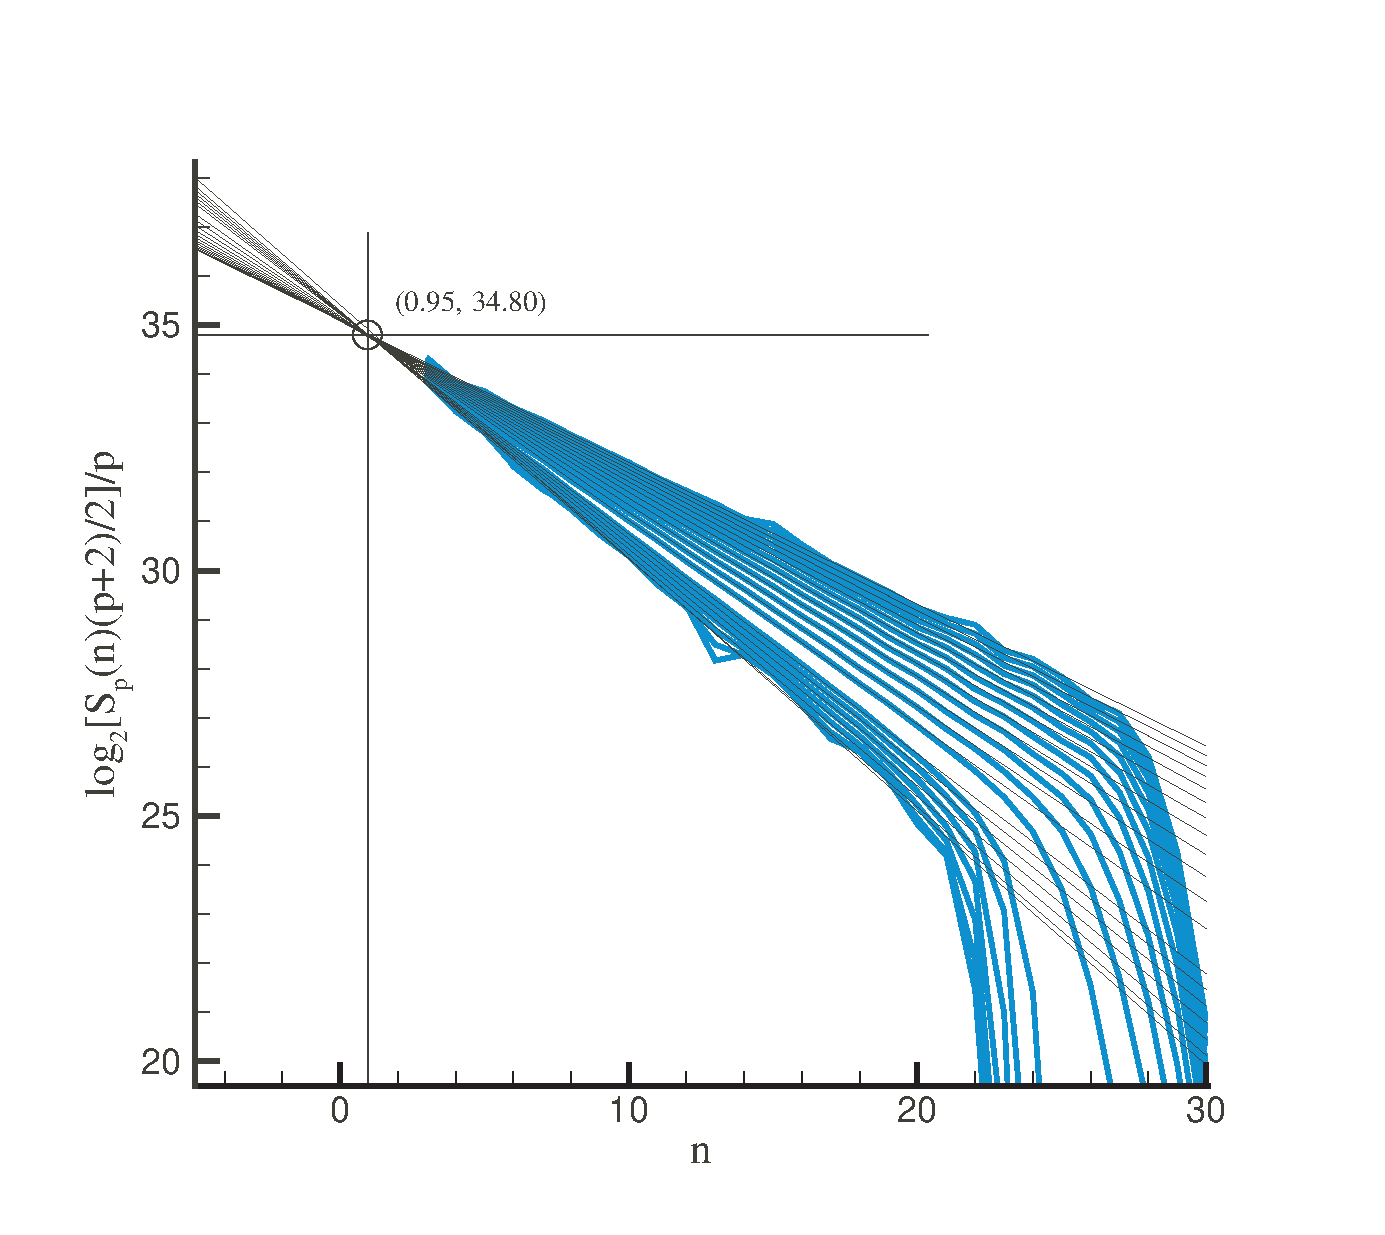
\includegraphics[width=4in]{at_focus.eps}
    \end{center}
    \caption{Rescaled structure function of Run 9 from Table \ref{table: app Sabra table} (Sabra). The functions can be formed because we have found universal coefficients.  $p = [-1.75, -1.5, \cdots, -0.5, -0.25, 0, 0.5, 1.0, \cdots, 11.5, 12.0]$} \label{fig: at focus}
\end{figure}

\subsection{The Limit of $p \rightarrow 0$}

Figure \ref{fig: at epsilon}.a show where $p = 0$ would be in the graph of rescaled structure functions.  This is due to (\ref{eq: log similarity formula 2}) involving a division by zero for $p = 0$.  Nonetheless, we can define a rescaled structure function for $p = 0$ through a limiting process.  Figure \ref{fig: at epsilon}.b clearly suggest that there are no problems for small $p$.  On the right hand side of (\ref{eq: log similarity formula 2}) it is the factor $\zeta_p/p$ that causes the problem.  Since $\zeta_0 = 0$, L'Hopitals rule can be applied.  In fact, the singularity at $p = 0$ is removable. We implement L'Hopitals rule for the data by means of a difference quotient:
\begin{equation}
    \lim_{p \rightarrow 0}\tilde{S}_p = \lim_{p \rightarrow 0}\frac{\tilde{S}_p - \tilde{S}_{-p}}{2p}.
\end{equation}
where
\begin{equation}
    \tilde{S}_p = \frac{1}{p}\ln\left(\frac{S_{p}(n)(p+2)}{2}\right).
\end{equation}

\begin{figure}[!hpt]
    \hspace{1.5in}{\centering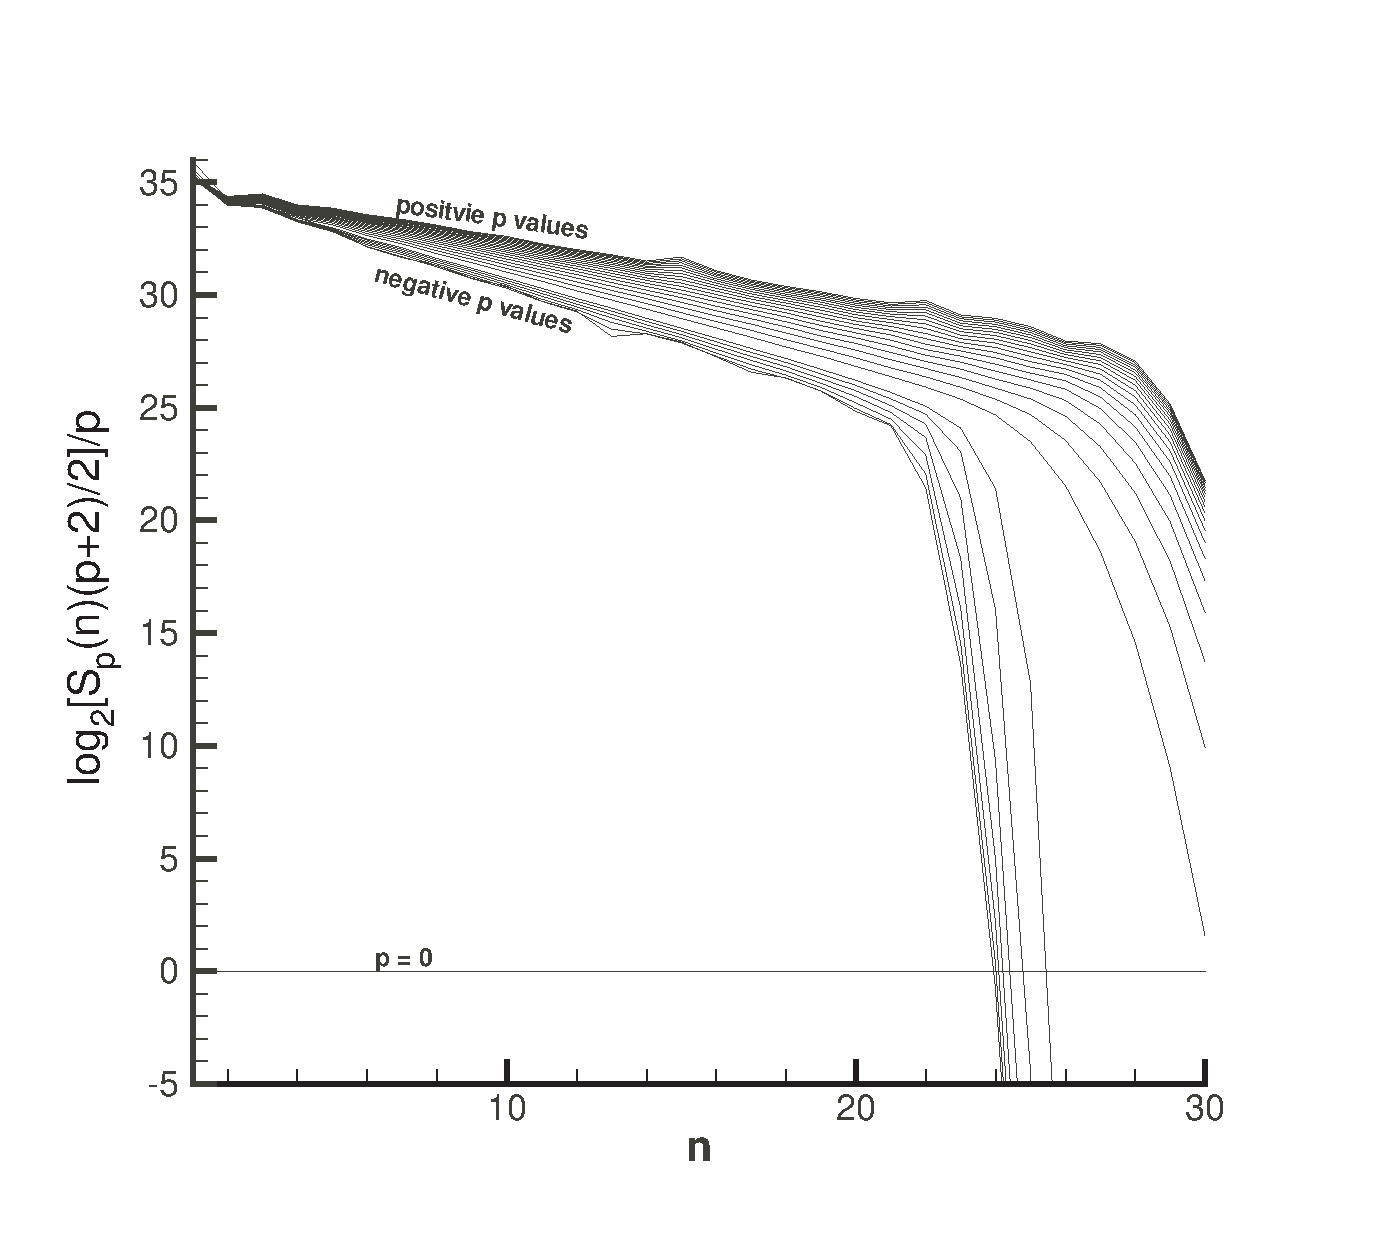
\includegraphics[width=4in]{tt_epsilon_with_0.eps}}\\

    \hspace{1.5in}{\centering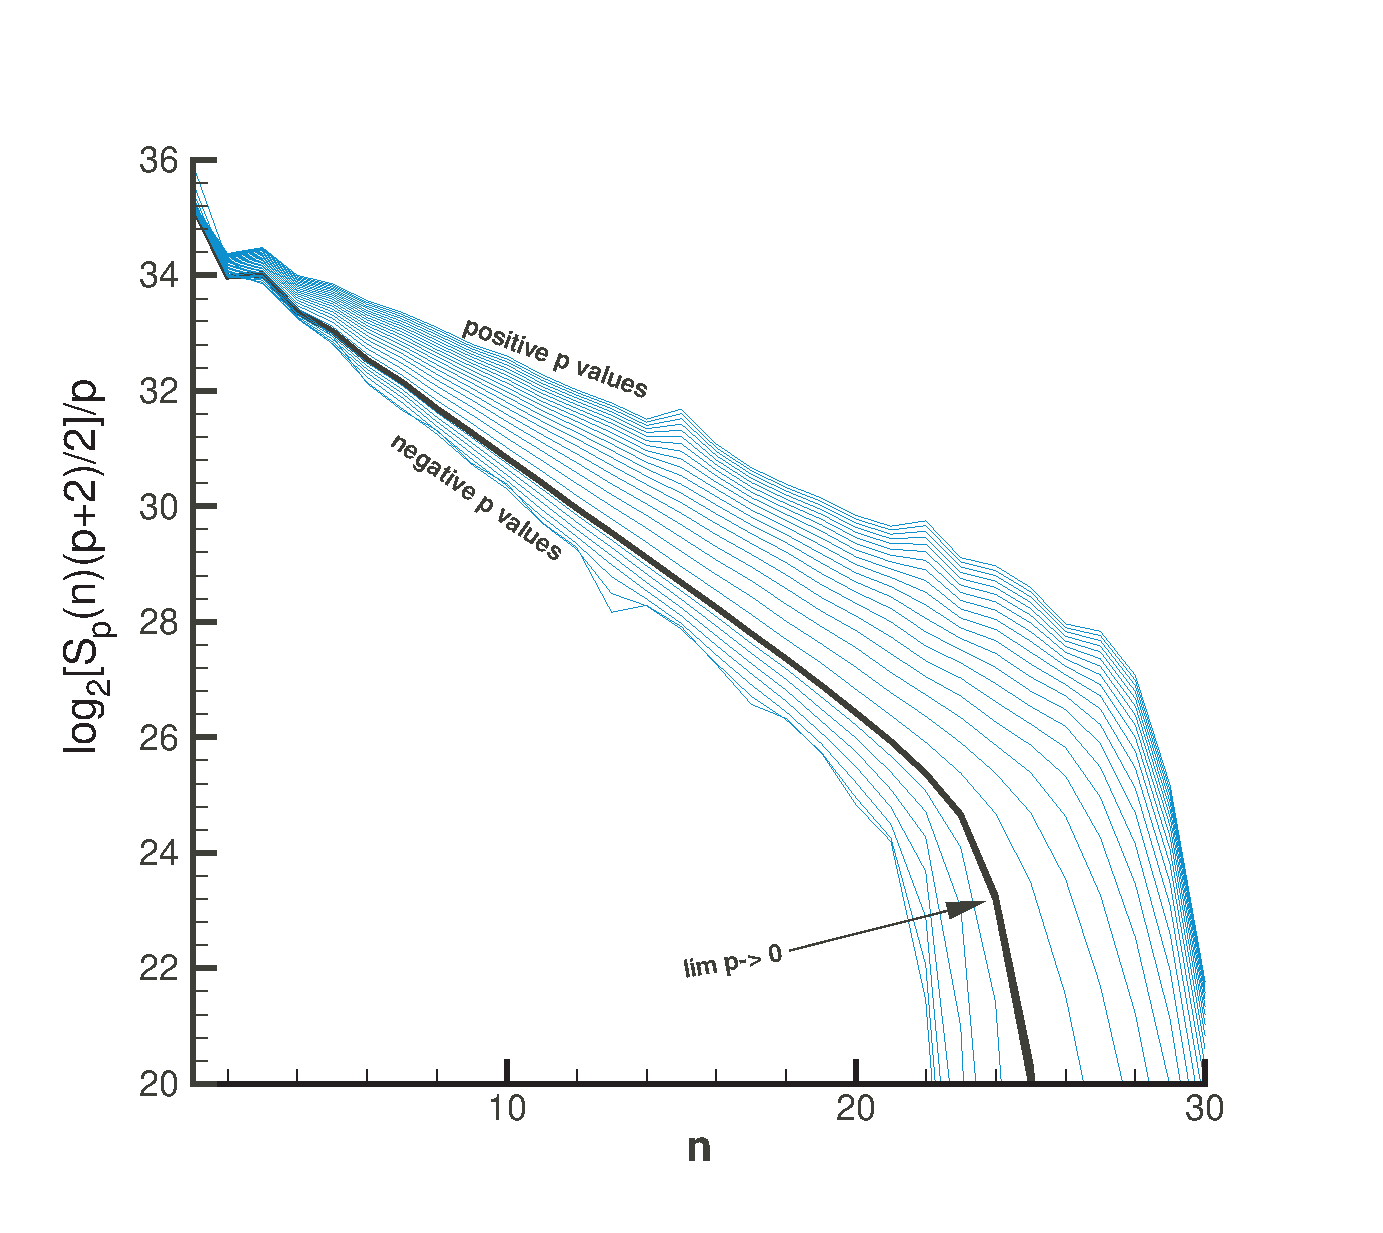
\includegraphics[width=4in]{tt_epsilon.eps}}
    \caption{Rescaled structure function of Run 9 from Table \ref{table: app Sabra table} (a) with $p = 0$ included. Note the gap between the negative and positive $p$ values. (b) as $p \rightarrow 0$  where $0.1 \geq p \geq 0.01$. Clearly a limit exists.} \label{fig: at epsilon}
\end{figure}

%\begin{equation}
%    \zeta_{p} - \frac{p}{3} = \frac{a}{3\beta(\beta-1)}\left[3(p+2)^{\beta} + (2^{\beta} - 5^{\beta})(p+2) + 2 \times5^{\beta} - 5\times2^{\beta} \right] \label{eq: Zetap}.
%\end{equation}

\vspace{2in}

\section{Graphically Measured Collapse}

Figure \ref{fig: all plots} show log-log plots of the radial profile $P_0(r;n)$ for $n$ ranging from 3 to 20.  As described in Chapter \ref{ch:self similarity of the joint pdf}, these graphs can be made to collapse by a similarity transformation.  Specifically, rigid horizontal shifts together with linear horizontal stretching.  Both shifts and stretching can be measured.  The process is as follows.  We first select one reference shell in the middle of the inertial range.  Let that be $n=12$.  The graphical objects corresponding to each of the other shells are then shifted rigidly and stretched horizontally so that the graphs match that of $P_0(r;12)$ as shown in Figures \ref{fig: s4and5with12} through \ref{fig: s19and20with12}.  Because the axes from Figure \ref{fig: all plots} are attached to $P_0(r;n)$ we can readily identify the vertical shift.  It is listed in Table \ref{table: measurements}.  We can also identify matching abscissa on the fixed and transformed scale.  The horizontal bars in Figure \ref{fig: s4and5with12} through \ref{fig: s19and20with12} are included for this purpose.  The corresponding abscissa pairs are listed in Table \ref{table: measurements}.  Since the transformation is linear only two values are needed for each $n$.  From these values we calculate the horizontal stretching factor $A$ and shift $B$, i.e.
\begin{equation}
	x_{stretched} = Ax_{f} + B
\end{equation}
Say $a$ and $b$ are two points on the fixed axis corresponding to $c$ and $d$ on the stretched axis, then
\begin{eqnarray}
	c & = & Aa + B \\
	d & = & Ab + B.
\end{eqnarray}
So that,
\begin{eqnarray}
	A & = & \frac{a-b}{c-d} \\
	B & = & \frac{bc-ad}{b-a}.
\end{eqnarray}
Figure \ref{fig: shifts} shows the vertical and horizontal shifts as functions of $n$.  We observe that both are linear functions of $n$ as called for by the theory.  The scatter around the regression line is in part due to the matching of the graphical objects being done manually.  The theory does provide analytical formulas to do a computational collapse.  However, the data we obtained contained too much statistical noise.  Therefore, we were not able to use the analytical formulas.  The vertical shift is also shown.  It forms a straight line on log-log scales.  Consequently, the stretching is a power law in $(n-n_0)$ just as predicted by the theory.  The slope is $1/\beta$ and we obtain $\beta = 1.23$ from the regression line.

\begin{table}[!htp]
    \begin{center}
    \caption{Measurements for scaling individual radial profiles.  Shell 12 is selected as the radial profile to be scaled to.  The fixed scale refers to the Shell 12 axis. The first pair of fixed and stretched scales refers to the initial alignment of the horizontal axis.  The second pair refers to the terminal alignment of the horizontal axis.}
    \begin{tabular}{||c|c|c|c|c|c||} \hline	
        \multicolumn{6}{|c|}{\emph{Measurements for Graphical Collapse}} \\ \hline \hline
        Shell & Fixed Scale & Stretched Scale & Fixed Scale & Stretched Scale & Vertical Shift \\
        \hline
        \hline
        3   &   15   &   22.2    &   21.1    &   24&     7\\
        4   &   16.2 &   22    &   22.1    &   24  &      6.2\\
        5   &   15.6 &   21    &   23.1    &   24  &      5.8\\
        6   &   16   &   21      &   22.8    &   24&      5.6\\
        7   &   14.8 &   19    &   23.2    &   24  &   3.7\\
        8   &   15.8 &   19    &   23.3    &   24  &   3.2\\
        9   &   15.6 &   18    &   23.5    &   24  &   1.8\\
        10   &   15.7&   17    &   23.6    &   24  &   1.2\\
        11   &   15.2&   16    &   23.8    &   24  &   0.8\\
        13   &   15.5&   15    &   24.3    &   24  &   -0.7\\
        14   &   17  &   15.7    &   24    &   23.6  &   -1.6\\
        15   &   17  &   15.2    &   24    &   24.3  &   -2.4\\
        16   &   18  &   15.6    &   24    &   23.3  &   -2.8\\
        17   &   18  &   15.2    &   24    &   23.1  &   -3.9\\
        18   &   19  &   16      &   24    &   22.8  &   -4.3\\
        19   &   19  &   15.1    &   24    &   22.7  &   -5.8\\
        20   &   20  &   16.1    &   24    &   22.6  &   -6.5\\
        \hline
        \hline
    \end{tabular}
    \end{center}
    \label{table: measurements}
\end{table}


\begin{figure}[!hpt]
    \begin{center}
     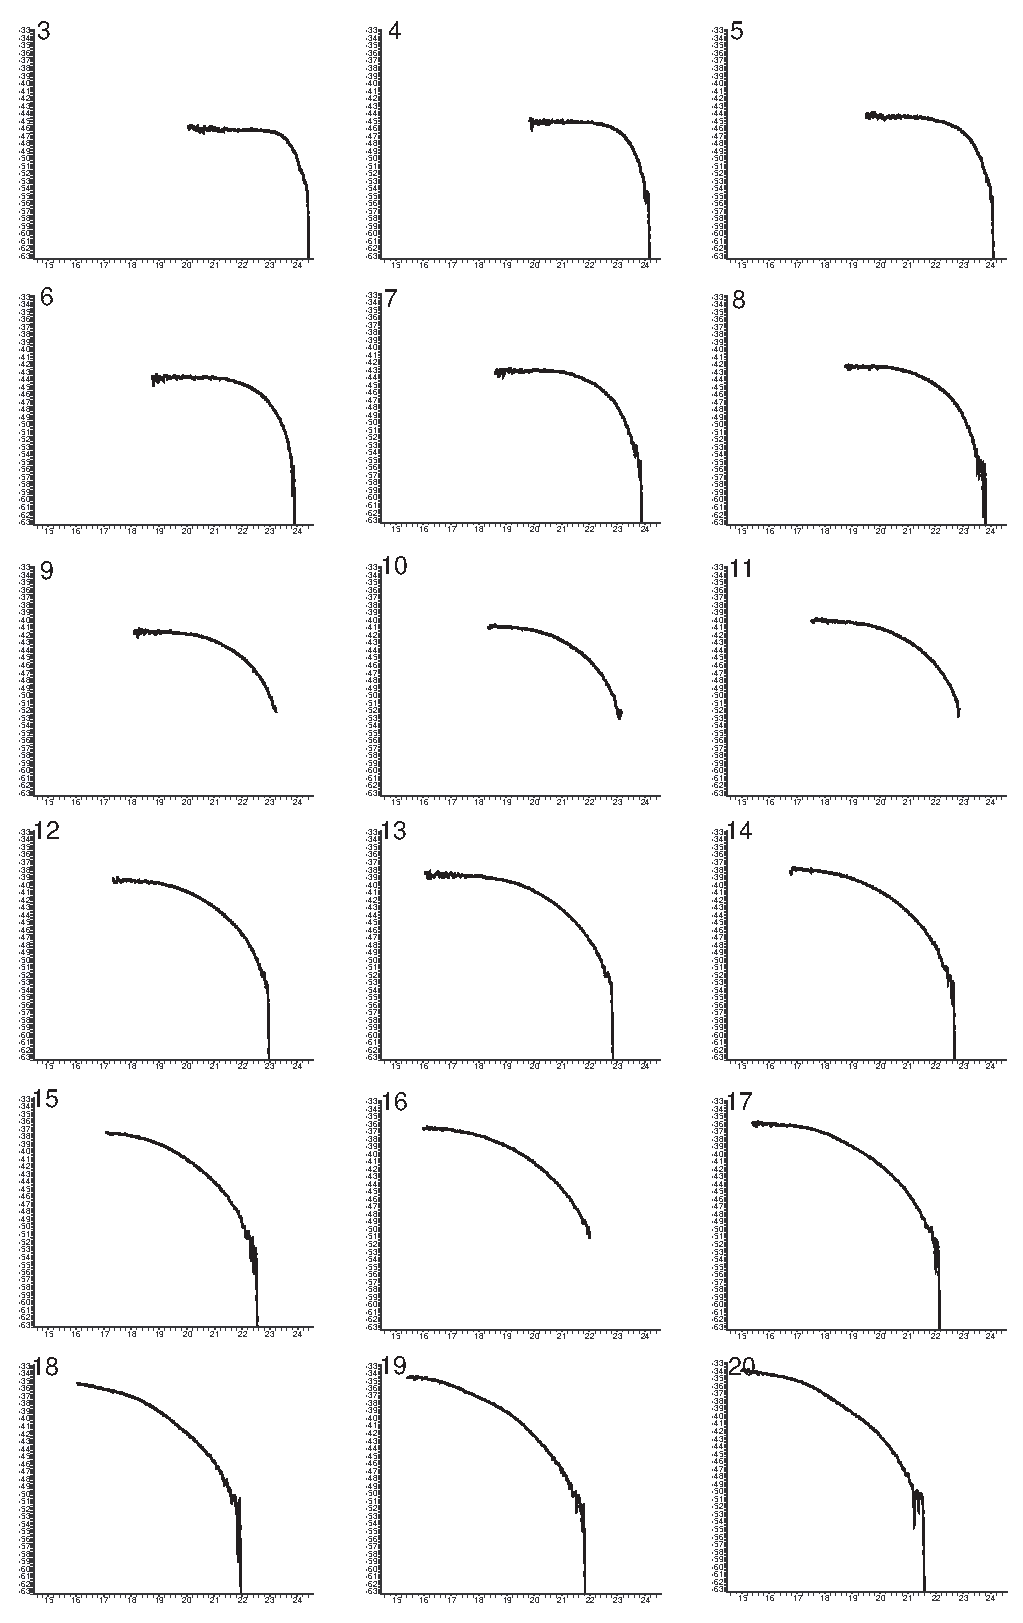
\includegraphics[width=4in]{allplots.eps}
     \end{center}
  \caption{Individual plots of each of the radial profiles that have a similar curve. The radial profiles $P_0(r;n)$ plotted on log-log scales for $3\leq n \leq 20$ for Sabra Run 9.} \label{fig: all plots}
\end{figure}

\begin{comment}
\begin{figure}[!hpt]
    \begin{center}
     \includegraphics[width=4in]{s4and5with12.eps}
     \end{center}
  \caption{(a) Collapse of $P_0(r;4)$ onto $P_0(r;12)$ using horizontal and vertical shift s together with horizontal stretching.  The vertical bars correspond to the numbers in Table (b) collapse of $P_0(r;5)$ onto $P_0(r;12)$.} \label{fig: s4and5with12}
\end{figure}

\begin{figure}[!hpt]
    \begin{center}
     \includegraphics[width=4in]{s6and7with12.eps}
     \end{center}
  \caption{(a) Collapse of $P_0(r;6)$ onto $P_0(r;12)$ (b) collapse of $P_0(r;6)$ onto $P_0(r;12)$.} \label{fig: s6and7with12}
\end{figure}

\begin{figure}[!hpt]
    \begin{center}
     \includegraphics[width=4in]{s8and9with12.eps}
     \end{center}
  \caption{(a) Collapse of $P_0(r;8)$ onto $P_0(r;12)$ (b) collapse of $P_0(r;9)$ onto $P_0(r;12)$.} \label{fig: s8and9with12}
\end{figure}

\begin{figure}[!hpt]
    \begin{center}
     \includegraphics[width=4in]{s10and11with12.eps}
     \end{center}
  \caption{(a) Collapse of $P_0(r;10)$ onto $P_0(r;12)$ (b) collapse of $P_0(r;11)$ onto $P_0(r;12)$.} \label{fig: s10and11with12}
\end{figure}

\begin{figure}[!hpt]
    \begin{center}
     \includegraphics[width=4in]{s13and14with12.eps}
     \end{center}
  \caption{(a) Collapse of $P_0(r;13)$ onto $P_0(r;12)$ (b) collapse of $P_0(r;14)$ onto $P_0(r;12)$.} \label{fig: s13and14with12}
\end{figure}

\begin{figure}[!hpt]
    \begin{center}
     \includegraphics[width=4in]{s15and16with12.eps}
     \end{center}
  \caption{(a) Collapse of $P_0(r;15)$ onto $P_0(r;12)$ (b) collapse of $P_0(r;16)$ onto $P_0(r;12)$.} \label{fig: s15and16with12}
\end{figure}

\begin{figure}[!hpt]
    \begin{center}
     \includegraphics[width=4in]{s17and18with12.eps}
     \end{center}
  \caption{(a) Collapse of $P_0(r;17)$ onto $P_0(r;12)$ (b) collapse of $P_0(r;18)$ onto $P_0(r;12)$.} \label{fig: s17and18with12}
\end{figure}

\begin{figure}[!hpt]
    \begin{center}
     \includegraphics[width=4in]{s19and20with12.eps}
     \end{center}
  \caption{(a) Collapse of $P_0(r;19)$ onto $P_0(r;12)$ (b) collapse of $P_0(r;20)$ onto $P_0(r;12)$.} \label{fig: s19and20with12}
\end{figure}

\begin{figure}[!hpt]
    \begin{center}
     \includegraphics[width=2.5in]{shifts.eps}
     \end{center}
  \caption{Graphs of (a) horizontal shift (b) vertical shift and (c) the horizontal stretching factor with regression lines fitted to the data } \label{fig: shifts}
\end{figure}

\section{Extracting the Theoretical Parameters}

In the theoretical formulas, there are four unknown constants that we must find, namely, $\beta$, $a$, $C_3$ and $n_0$. In principle, we also need $\zeta_3$, but we have already found it to be very close to one therefore, we assume $\zeta_3 \equiv 1$ in accordance with the four-fifth's law.  There are several ways to extract the constants from the data. We have seen one way of extracting $n_0$, $C_3$, and $\beta$ in sections 10.1 and 10.2. Now, we discuss two other methods for attaining these parameters.

The first involves divided differences based on the rescaled structure functions.  This method goes through step-by-step eliminating unknowns till $\beta$ is the last unknown available.  Then the method filters back through to give us values for the other unknowns.

The second method uses cumulants.  Through this method, we use ratios and graphs to determine the values.  Using both methods gives us a way to check the accuracy of the values.

\subsection{Divided Differences}

We will use two intermediate variables, $m_{p}$ and $R_{p}$.  Using these variables we will be able to extract $\beta$ which will in turn yield $a$, and we will be able to check the values of $n_{0}$ and $C_{3}$.

To find $m_{p}$, we need to rearrange (\ref{eq: log similarity formula 2}). Moving $\ln (5/2 S_{3})$ from the left and right hand side, we have
\begin{eqnarray}
    m_{p} & \equiv & \frac{3}{p}\ln\left(\frac{S_{p}(n)(p+2)}{2}\right) - \ln \left(\frac{5}{2}S_{3}\right) \nonumber\\
    & = & \ln\left(\frac{5C_{3}}{2}\right) -\frac{3}{p}\zeta_{p}(n-n_{0})\ln2 - \ln \left(\frac{5}{2}S_{3}\right) \nonumber\\
    & = & \ln\left(\frac{5C_{3}}{2}\right) -\frac{3}{p}\zeta_{p}(n-n_{0})\ln2 - \ln\left(\frac{5}{2}C_{3}2^{-\zeta_{3}(n-n_{0})}\right) \nonumber\\
    & = & \ln\left(\frac{5C_{3}}{2}\right) -\frac{3}{p}\zeta_{p}(n-n_{0})\ln2 - \ln\left(\frac{5}{2}C_{3}\right) + \zeta_{3}(n-n_{0}) \ln2 \nonumber\\
    & = & -\frac{3}{p}\zeta_{p}(n-n_{0})\ln2  + \zeta_{3}(n-n_{0}) \ln2
\end{eqnarray}
or, with $\zeta_3 = 1$:
\begin{equation}
    m_p =  \left(1-\frac{3}{p}\zeta_{p}\right)(n-n_{0})\ln2. \label{eq: mp}
\end{equation}
Through this process we have eliminated $C_{3}$ and are left with three unknowns. Note, theoretically $m_3 \equiv 0$.

\begin{figure}[!hpt]
    \begin{center}
    \includegraphics[width=4in]{at_mp_vs_m2.eps}
    \end{center}
    \caption{Plot of $m_p$ vs. $m_2$. Straight lines are superimposed over the different data sets. The data sets are represented by squares.} \label{fig: at mp vs m2}
\end{figure}

The theoretical expression (\ref{eq: mp}) vanishes for $n = n_0$ for all $p$ and is linear in $n - n_0$.  Consequently, $(m_2, m_p)$ constitutes a parameteric representation for a straight line with $(n - n_0)$ as the parameter.  This line passes through (0,0) regardless of the value of $p$.

Figure \ref{fig: at mp vs m2} shows $m_{p}$ vs. $m_{2}$. We substitute in the regression line values we found previously for $\zeta_p$.  Using this figure, the power laws are tested once more.  The straight lines through the points are a clear indication that the power laws do hold.  Note, that all lines meet at $(0,0)$. Thus, the ratio of $m_{p}$ and $m_{2}$ is independent of $n-n_{0}$ in the power law regime, i.e.
\begin{equation}
    \frac{m_{p}}{m_{2}} = \frac{\left(1-\frac{3}{p}\zeta_{p}\right)(n-n_{0})\ln2}{\left(1-\frac{3}{2}\zeta_{2}\right)(n-n_{0})\ln2}.
\end{equation}
This eliminates $n_{0}$ from the equation. We will call the reduced ratio $R_p$, i.e.
\begin{equation}
    R_p =  \frac{\left(1-\frac{3}{p}\zeta_{p}\right)}{\left(1-\frac{3}{2}\zeta_{2}\right)} \label{eq: rp in process}
\end{equation}

Next, we substitute the expressions for $\zeta_{p}$ and $\zeta_{2}$ into (\ref{eq: rp in process}). In doing so, we find that $R_p$ is independent of $a$,
\begin{eqnarray}
     R_{p} & = & \frac{\frac{a}{p\beta(\beta-1)}\left(3(p+2)^{\beta} + (2^{\beta}-5^{\beta})(p+2) + 2\times5^{\beta}-5\times2^{\beta}\right)}{\frac{a}{2\beta(\beta-1)}\left(3(2+2)^{\beta} + (2^{\beta}-5^{\beta})(2+2) + 2\times5^{\beta}-5\times2^{\beta}\right)} \nonumber\\
     & = & \frac{2\left(3(p+2)^{\beta} + (2^{\beta}-5^{\beta})(p+2) + 2\times5^{\beta}-5\times2^{\beta}\right)}{p\left(3\times4^{\beta} - 2^{\beta}-2\times5^{\beta}\right)}. \label{eq: rp}
\end{eqnarray}
$R_{p}$ is an expression that can be computed from the data for each value of $n$; see Figure \ref{fig: at rp}. The expression should theoretically be independent of $u$. As one would expect, the larger $p$ becomes the more statistical noise we observe.

\begin{figure}[!hpt]
    \begin{center}
    \includegraphics[width=4in]{at_rp.eps}
    \end{center}
    \caption{\ref{eq: rp} for $5\geq n \geq 20$.} \label{fig: at rp}
\end{figure}

In principle, (\ref{eq: rp}) should allow us to solve for $\beta$. In order to determine $\beta$, we first average each $R_{p}$ over $n$.  After this, we determine the different standard deviations which gives a measure for the statistical noise.  Once done, we can plot various values of $\beta$, restricted to $0<\beta<3$.  Given the average $R_{p}$ and the standard deviation of $R_{p}$, we can estimate the $\beta$ value that best matches the data.  We find $\beta \simeq 1.6$.

\begin{figure}[!hpt]
    \begin{center}
        \includegraphics[width=4in]{at_ave_rp.eps}
    \end{center}
    \caption{Average $R_p$ with standard deviation as error bars.  Surrounding curves are different values of $\beta$ computed to find the best fit.}  \label{fig: at average rp beta}
\end{figure}

Now that we know $\beta$ we can find $a$ from (\ref{eq: mp}).  If we define
\begin{equation}
    K_{p} = \frac{1}{a}\left(\zeta_{p} - \zeta_{3}\frac{p}{3}\right)
\end{equation}
then
\begin{eqnarray}
    m_{p} & = & \left(\frac{3}{p}\zeta_{p} - 1\right)(n-n_0)\ln2 \nonumber \\
    & = & \left(\frac{3}{p}\left(aK_{p} + \frac{p}{3}\right) - 1\right)(n-n_0)\ln2 \nonumber \\
    & = & \frac{3}{p}aK_{p}(n-n_0)\ln2.
\end{eqnarray}
Therefore,
\begin{equation}
    a = \frac{m_{p}p}{3K_{p}(n-n_0)\ln2}. \label{eq: a}
\end{equation}
For $\beta = 1.6$, we find $a = -0.11$.

\begin{figure}[!htp]
    \begin{center}
        \includegraphics[width = 4in]{at_find_a_beta_160.eps}
    \end{center}
    \caption{Using the value we find in (\ref{eq: rp}), we plug into (\ref{eq: a}).  The slope of the inertial range yields the value of $a$.}
\end{figure}

\subsection{Cumulants}

Another technique to determine the four parameters in the similarity theory is to utilize cumulants. While moments are generated from a series expansion of the first characteristic function the Fourier transform of the pdf, cumulants are are generated from the second characteristic function. Specifically, suppose we have a random variable $-\infty < X < \infty$ with a pdf $f(x)$ then the Fourier transform of $f$ is the first characteristic function
\begin{equation}
	\hat{F}(s) = \int^{\infty}_{-\infty}f(x)e^{isx}dx \label{eq: fourier transform}
\end{equation}
This function has a MacLaurin series which one finds by expanding the exponential function $e^{isx}$,
\begin{eqnarray}
	\hat{F}(s) & = & \int^{\infty}_{-\infty} f(x) \sum^{\infty}_{k = 0}\frac{(isx)^k}{k!}dx \nonumber \\
	& = & \sum^{\infty}_{k = 0}\frac{(is)^k}{k!}\int^{\infty}_{-\infty} x^k f(x)dx \nonumber \\
	& = & \sum^{\infty}_{k = 0}\frac{(is)^k}{k!}\mathcal{M}_k,
\end{eqnarray}
where $\mathcal{M}_k = \langle X^k \rangle$ are the moments.  The second characteristic function is then defined as
\begin{equation}
	\hat{G}(s) = \log \left(\hat{F}(s)\right).
\end{equation}
Its expansion reads
\begin{equation}
	\hat{G}(s) = \sum^{\infty}_{k = 0}Q_k \frac{(is)^k}{k!} \label{eq: cumulant series}
\end{equation}
where the coefficients, $Q_k$ are called the cumulants of the random variable, $X$, or the pdf, $f$.

\vspace{2in}

\subsubsection{Defining Cumulants}

The cumulants, $Q_k$, are related to moments through formulas that can be found in \cite{Kendall69}. We use the first three of these formulas
\begin{eqnarray}
    Q_{1} \equiv \langle\langle X \rangle\rangle & = & \langle X \rangle \label{eq: Q1 theory} \\
    Q_{2} \equiv \langle\langle X^2 \rangle\rangle & = & \langle X^2 \rangle - \langle X \rangle^{2} \label{eq: Q2 theory} \\
    Q_{3} \equiv \langle\langle X^3 \rangle\rangle & = & \langle X^3 \rangle - 3\langle X^2 \rangle\langle X \rangle + 2\langle X \rangle^{3} \label{eq: Q3 theory}.
\end{eqnarray}

These formulas show how we can compute the cumulants from computational data i.e., the moments of $X$.  From (\ref{eq: cumulant series}) follows
\begin{equation}
    Q_k \equiv \left.\left[(-i)^k\left(\frac{d}{ds}\right)^{k}\hat{G}(s)\right]\right|_{s = 0}. \label{eq: cumulant def}
\end{equation}
Let us define the pdf for the shell amplitude, $A$, as $\phi$, i.e.,
\begin{equation}
    \phi(x)dx = Pr\{x\leq A\leq x+ dx\}.
\end{equation}
Moreover, let $\psi$ be the pdf for $\ln A$, i.e.,
\begin{equation}
    \psi(y)dy = Pr\{y\leq \ln A\leq y+ dy\}.
\end{equation}
There is, of course, a relationship between $\phi$ and $\psi$.  We found it previously in Chapter \ref{ch:self similarity of the joint pdf}, namely
\begin{equation}
    \phi(x) = \frac{\psi(\ln x)}{x}.
\end{equation}
By a change of variables,  $x = e^{t}$, we obtain $\psi$ in terms of $\phi$:
\begin{equation}
    \psi(t) = e^t \phi(e^t).
\end{equation}
The characteristic function of $\hat{\Psi}$ is then obtained through a Fourier integral as follows:
\begin{eqnarray}
    \hat{\Psi}(s) & = & \int^{\infty}_{-\infty}\psi(x)e^{isx}dx \nonumber \\
    & = & \int^{\infty}_{-\infty}e^x\phi(e^x)e^{ixs}dx \nonumber \\
    & = & \int^{\infty}_{-\infty}\phi(e^x)e^{(is+1)x}dx .
\end{eqnarray}
By substitution $u = e^x$ and $du = e^xdx$, we can express $\hat{\Psi}(s)$ as a Mellin transform, i.e.,
\begin{eqnarray}
    \hat{\Psi}(s) & = & \int^{\infty}_{0}\phi(u)u^{is}du \nonumber \\
    & = & \int^{\infty}_{0}\phi(u)u^{is+1}\frac{du}{u} \nonumber \\
    & = & \mathcal{M}[\phi(u); is + 1].
\end{eqnarray}
The Mellin transform of $\phi$ brings us back to the power laws for the inertial range,
\begin{equation}
     \hat{\Psi}(s) = S_{is}(\ell) =  C_{is}\ell^{\zeta_{is}}. \label{eq: at cap psi}
\end{equation}
We notice that the order index $p$, i.e. in $C_p$ and $\zeta_p$, is now replaced by the complex value $is$.  Thus, for (\ref{eq: at cap psi}) to be of use, we must have analytic formulas for $C_p$ and $\zeta_p$.  Otherwise, we cannot extend $C_p$ and $\zeta_p$ into the complex plane. The theory from Chapter \ref{ch:a new theory} is helpful in this regard.

\subsubsection{Applying Cumulants}

It follows from (\ref{eq: at cap psi}) that
\begin{equation}
    \ln \hat{\Psi}(s) = \ln C_{is} + \zeta_{is}\ln \ell
\end{equation}
where the expansion
\begin{equation}
    \ln \hat{\Psi}(s) = \sum^{\infty}_{k = 0}Q_k\frac{(is)^k}{k!}
\end{equation}
provides the cumulants of $\ln A_n$.

Using our previous shell notation (\ref{eq: new sfp}) we have
\begin{equation}
    \hat{\Phi}_{n}(s) = \mathcal{M}\left[\phi_{n}(u);is+1\right] = S_{is}(n) = C_{is}2^{-\zeta_{is}(n-n_{0})}. \label{eq: psi which is sfp}
\end{equation}
For simplicity, let $\eta = (n-n_{0})\ln 2$, so that (\ref{eq: psi which is sfp}) reads
\begin{equation}
    S_{is}(n) = C_{is}e^{-\eta\zeta_{is}} . \label{eq: psi with eta}
\end{equation}
Then, using (\ref{eq: cumulant series}), (\ref{eq: cumulant def}), and (\ref{eq: psi which is sfp}), we obtain
\begin{equation}
    Q_m = \left.\left[\left(-i\frac{d}{ds}\right)^{m}\left(\ln C_{is} - \eta\zeta_{is}\right)\right]\right|_{s = 0},
\end{equation}
which clearly shows that all cumulants are linear functions of $\eta$ in the inertial range.

The first cumulant, $m=1$, is
\begin{eqnarray}
    Q_{1} & \equiv & \left.\left[\left(-i\frac{d}{ds}\right)^{1}\ln \left(C_{is}e^{-\eta\zeta_{is}}\right)\right]\right|_{s = 0} \nonumber \\
    & = & \left.\left[-i\left(\frac{iC_{is}'}{C_{is}} - i\eta\zeta_{is}'\right)\right]\right|_{s=0} \nonumber \\
    & = & \left.\left[\frac{C_{is}'}{C_{is}} - \eta\zeta_{is}'\right]\right|_{s=0} .
\end{eqnarray}
Since $C_0 \equiv 1$, we obtain
\begin{equation}
    Q_{1} =  C_{0}' - \eta\zeta_{0}' .
\end{equation}
Using the same process, we find $Q_{2}$,
\begin{eqnarray}
    Q_{2} & \equiv & \left.\left[\left(-i\frac{d}{ds}\right)^{2}\ln \left(C_{is}e^{-\eta\zeta_{is}}\right)\right]\right|_{s = 0} \nonumber \\
    & = & \left.\left[-i\left(\frac{iC_{is}C_{is}'' - iC_{is}'^{2}}{C_{is}^{2}} - i\eta\zeta_{is}''\right)\right]\right|_{s=0} \nonumber \\
    & = & \left.\left[\frac{C_{is}C_{is}'' - C_{is}'^{2}}{C_{is}^{2}} - \eta\zeta_{is}''\right]\right|_{s=0} .
\end{eqnarray}
Again, using $C_0 \equiv 1$, we have
\begin{equation}
    Q_{2} =  C_{0}'' - C_{0}'^{2} - \eta\zeta_{0}'' .
\end{equation}
For $Q_{3}$,
\begin{eqnarray}
    Q_{3} & \equiv & \left.\left[\left(-i\frac{d}{ds}\right)^{3}\ln \left(C_{is}e^{-\eta\zeta_{is}}\right)\right]\right|_{s = 0} \nonumber \\
    & = & \left.\left[-i\left(\frac{iC_{is}C_{is}'''-iC_{is}''C_{is}'}{C_{is}^{2}} - 2i\frac{C_{is}^{2}C_{is}''-C_{is}'^{3}}{C_{is}^{4}} - i\eta\zeta_{is}'''\right)\right]\right|_{s=0} \nonumber \\
    & = & \left.\left[\frac{C_{is}C_{is}'''-C_{is}''C_{is}'}{C_{is}^{2}} - 2\frac{C_{is}^{2}C_{is}''-C_{is}'^{3}}{C_{is}^{4}} - \eta\zeta_{is}'''\right]\right|_{s=0} \nonumber \\
    & = &=  C_{0}'''-C_{0}''C_{0}' - 2\left(C_{0}''-C_{0}'^{3}\right) - \eta\zeta_{0}''' .
\end{eqnarray}

Using the theoretical formulas for $\zeta_p$ and $C_p$ from \cite{Melander2007} we calculate the derivatives $C_{0}^{(m)}$ and $\zeta_{0}^{(m)}$. As a result we have the cumulants expressed in term of the parameters $a$, $\beta$, $C_3$, and $n_0$,
\begin{equation}
    Q_{1} = -\frac{1}{2} + \frac{1}{3}\ln \left(\frac{5}{2}C_{3}\right) -  \left(\frac{a}{3\beta(\beta-1)}  \left(\frac{5}{2}\beta2^{\beta}+2^{\beta}-5^{\beta}\right)+\frac{1}{3}\right)(n-n_{0})\ln2, \label{eq: Q1}
\end{equation}
\begin{equation}
    Q_{2} = \frac{1}{4}-\frac{1}{4}a2^{\beta}(n-n_{0})\ln2, \label{eq: Q2}
\end{equation}
and
\begin{equation}
    Q_{3} = -\frac{1}{4}-\frac{1}{8}a2^{\beta}(\beta-2)(n-n_{0})\ln2. \label{eq: Q3}
\end{equation}

Note that $Q_1$ and $Q_2$ define all four parameters.  The higher orders do not bring any new information, but also do not contradict $Q_1$ and $Q_2$ \cite{Kendall69}. We rearrange cumulant formulas for easier graphical interpretation as follows
\begin{equation}
    3Q_{1} + \frac{3}{2} = \ln \left(\frac{5}{2}C_{3}\right) -  \left(\frac{a}{\beta(\beta-1)}  \left(\frac{5}{2}\beta2^{\beta}+2^{\beta}-5^{\beta}\right)+1\right)(n-n_{0})\ln2, \label{eq: 3Q1 p 3o2}
\end{equation}
\begin{equation}
    4Q_{2} - 1 = a2^{\beta}(n-n_{0})\ln2, \label{eq: 4Q2 m 1}
\end{equation}
and
\begin{equation}
    8Q_{3} + 2 = -a2^{\beta}(\beta-2)(n-n_{0})\ln2. \label{eq: 8Q3 p 2}
\end{equation}

The moment based cumulant formulas, i.e. (\ref{eq: Q1 theory}), (\ref{eq: Q2 theory}), (\ref{eq: Q3 theory}), with $X = \ln A_n$ and the derived cumulant formulas, i.e. (\ref{eq: Q1}), (\ref{eq: Q2}), (\ref{eq: Q3}) describe the same set of statistics.  We can calculate the moment based cumulants from the data to get the left hand sides of (\ref{eq: 3Q1 p 3o2}), (\ref{eq: 4Q2 m 1}), (\ref{eq: 8Q3 p 2}).  By extracting the regression lines, we can obtain the four unknown constants, $a$, $\beta$, $C_3$, and $n_0$.  Figure \ref{fig: at cumulant} displays the cumulants and their respective regression lines. Graphically, we find the value of $n_0$ by inspecting the zero crossings of $4Q_2 - 1$ and $8Q_3 + 2$. The former being statistically more accurate then the latter.

\begin{figure}[!hpt]
    \begin{center}
    \includegraphics[width=4in]{at_cumulant.eps}
    \end{center}
    \caption{Equations (\ref{eq: 3Q1 p 3o2}), (\ref{eq: 4Q2 m 1}), (\ref{eq: 8Q3 p 2}) plotted along with their respective regression lines.} \label{fig: at cumulant}
\end{figure}

The regression lines for the derived cumulant formulas can be written as
\begin{equation}
    Q_m = A_m + (n-n_0)B_m
\end{equation}
yields (\ref{eq: Q1}), (\ref{eq: Q2}), and (\ref{eq: Q3}). The data, i.e. Figure \ref{fig: at cumulant},
\begin{eqnarray}
    \tilde{Q}_{1} = 3Q_1 + \frac{3}{2} & = & \tilde{A}_{1} + n\tilde{B}_{1}  \\
    \tilde{Q}_{2} = 4Q_2 - 1 & = & \tilde{A}_{2} + n\tilde{B}_{2} \label{eq: 4q2} \\
    \tilde{Q}_{3} = 8Q_3 + 2 & = & \tilde{A}_{3} + n\tilde{B}_{3}  .
\end{eqnarray}
corresponding to (\ref{eq: 3Q1 p 3o2}), (\ref{eq: 4Q2 m 1}), and (\ref{eq: 8Q3 p 2}). While we may not know the specific values of $A_m$, $B_m$, we do know the values of $\tilde{A}_m$, $\tilde{B}_m$.

Now, we determine the ratios between $B_m$ and $\tilde{B}_m$. Starting with $m = 1$, we have
\begin{eqnarray}
    3Q_{1} + \frac{3}{2} & = & 3A_{1} + 3B_{1}(n-n_{0}) + \frac{3}{2} \nonumber \\
    & = & 3A_{1} + 3B_{1}n - 3B_{1}n_{0} + \frac{3}{2} = \tilde{A_{1}} + \tilde{B_{1}}n. \label{eq: 3Q1 p 3o2 with tildes}
\end{eqnarray}
Hence, $\tilde{B_{1}} = 3B_{1}$. We proceed to find the relationship between $\tilde{B_{2}}$ and $B_{2}$,
\begin{eqnarray}
    4Q_{2} - 1 & = & 4A_{2} + 4B_{2}(n-n_{0}) - 1 \nonumber \\
    & = & 4A_{1} + 4B_{2}n - 4B_{2}n_{0} - 1 = \tilde{A_{2}} + \tilde{B_{2}}n. \label{eq: 4Q2 m 1 with tildes}
\end{eqnarray}
Then, $\tilde{B_{2}} = 4B_{2}$. The relationship between $\tilde{B_{3}}$ and $B_{3}$ follows the previous steps. We find $\tilde{B_{3}} = 8B_{3}$. Now, we have all the equations and ratios we need to solve for the unknown constants.

\subsubsection{Solving for Parameters}

First, we will calculate $n_{0}$.  To accomplish this, we use (\ref{eq: 4Q2 m 1}) to obtain
\begin{equation}
    4Q_{2}(n_{0}) - 1 = -a2^{\beta}(n_{0}-n_{0})\ln 2  \label{eq: to go below}
\end{equation}
such that combing (\ref{eq: 4q2}) with (\ref{eq: to go below}) yields
\begin{equation}
    \tilde{A_{2}} + \tilde{B_{2}}n_{0} = 0
\end{equation}
\begin{equation}
    n_{0} = \frac{-\tilde{A_{2}}}{\tilde{B_{2}}}. \label{eq: found n0}
\end{equation}
Using the numerical values from the linear fits in Figure \ref{fig: at cumulant} for $\tilde{A}_2$ and $\tilde{B}_2$, we obtain $n_0 = 1.12$.

To find $C_{3}$, we use the same process with (\ref{eq: 3Q1 p 3o2}) and (\ref{eq: 3Q1 p 3o2 with tildes}). Letting $n = n_{0}$, we have
\begin{equation}
    3Q_{1}(n_{0}) + \frac{3}{2} = \ln \left(\frac{5}{2}C_{3}\right)
\end{equation}
then,
\begin{equation}
    \ln \left(\frac{5}{2}C_{3}\right) = \tilde{A_{1}} + \tilde{B_{1}}n_{0}
\end{equation}
so that
\begin{equation}
    C_{3} = \frac{2}{5}e^{\tilde{A_{1}} + \tilde{B_{1}}n_{0}} . \label{eq: found C3}
\end{equation}
Substituting in the numerical values for $\tilde{A}_1$ and $\tilde{B}_1$ along with the value we found for $n_0$, we find $C_3 =  0.84 \times 10^{31}$. Note this enormous value of $C_3$ is a consequences of the way we non-dimensionalized the shell model in Chapter \ref{ch:shell models}.  Essentially, we scaled our viscous unit by setting $\nu = 1$ and having enormous forcings. We can check that this $C_{3}$ is close to the $C_{3}$ we located in the rescaled structure function graph, see Figure \ref{fig: at focus}.  However, we need to remember that the number we found there was actually $\frac{1}{3}\log_{2}C_{3} = 34.8$. Using the cumulants, we find $\frac{1}{3}\log_{2}C_{3} = 34.2$. We do indeed find the values similar.

Next, we would like to find $a$ and $\beta$.  From (\ref{eq: 4Q2 m 1 with tildes}), we have
\begin{equation}
    4B_{2} = \tilde{B_{2}},
\end{equation}
so that
\begin{equation}
    4\left(\frac{-1}{4}a2^{\beta}\ln 2\right) = \tilde{B_{2}},
\end{equation}
and consequently,
\begin{equation}
    a = \frac{-\tilde{B_{2}}}{2^{\beta}\ln2} . \label{eq: found a}
\end{equation}
Now, we will substitute (\ref{eq: found a}) into $\tilde{B_{1}} = 3B_{1}$ from (\ref{eq: 3Q1 p 3o2 with tildes}). Solving for $\beta$, we obtain
\begin{eqnarray}
    \tilde{B_{1}} & = &   - 3\left(\frac{a}{3\beta(\beta-1)} \left(\frac{5}{2}\beta2^{\beta}+2^{\beta}-5^{\beta}\right)+\frac{1}{3}\right)\ln2  \nonumber \\
    & = & - \left(\frac{-\tilde{B_{2}}}{2^{\beta}\ln2}\cdot\frac{1}{\beta(\beta-1)} \left(\frac{5}{2}\beta2^{\beta}+2^{\beta}-5^{\beta}\right)+1\right)\ln2 \label{eq: found beta}
\end{eqnarray}
To solve for $\beta$, let us turn (\ref{eq: found beta}) into a function based solely on $\beta$.
\begin{equation}
    F(\beta) =  - \left(\frac{-\tilde{B_{2}}}{2^{\beta}\ln2}\cdot\frac{1}{\beta(\beta-1)} \left(\frac{5}{2}\beta2^{\beta}+2^{\beta}-5^{\beta}\right)+1\right)\ln2 - \tilde{B_{1}}
\end{equation}
The value of $\beta$ we are interested in is the root of $f(\beta) = 0$. This value is $\beta = 1.36$, see Figure \ref{fig: at f of beta}. We then take this $\beta$ value and substituting into (\ref{eq: found a}) to solve for $a$, we find $a = -0.13$

\begin{figure}[!hpt]
    \begin{center}
    \includegraphics[width=4in]{at_fofbeta.eps}
    \end{center}
    \caption{$F(\beta)$ solving for $f(\beta) = 0$. The root is $\beta = 1.3558$.} \label{fig: at f of beta}
\end{figure}

Ratios between higher order cumulant $Q_m$, $m \geq 2$ depend on $\beta$.  So, in principle $\beta$ is determined uniquely by the higher orders, but the statistical noise amplifies quickly as the order increases. As an illustration, we can check the value of $\beta$ by using the ratio of $Q_{2} - \frac{1}{4}$ to $Q_{3} + \frac{1}{4}$,
\begin{eqnarray}
    \frac{Q_{3} + \frac{1}{4}}{Q_{2} - \frac{1}{4}} & = & \frac{-\frac{1}{8}a2^{\beta}(\beta-2)(n-n_{0})\ln2}{-\frac{1}{4}a2^{\beta}(n-n_{0})\ln 2} \nonumber \\
    & = & \frac{\beta}{2} - 1 \nonumber \\
    \Rightarrow \beta & = & 2\left(\frac{Q_{3} + \frac{1}{4}}{Q_{2} - \frac{1}{4}} + 1\right) \label{eq: ratio solving for beta}
\end{eqnarray}
Here the right hand side should be independent of the shell number $n$ provided that the statistics have convergent and we are in the inertial range.  Graphically, we can examine (\ref{eq: ratio solving for beta}) three ways as illustrated by Figure \ref{fig: at ratio cumulants}.  The obvious route is to observe what the ratio looks like through the use of our cumulant data from (\ref{eq: 3Q1 p 3o2}), (\ref{eq: 4Q2 m 1}), (\ref{eq: 8Q3 p 2}), see Figure \ref{fig: at cumulant}.  This gives a rather jagged curve which does not give a clear indication of the value of $\beta$.  The next method we implement is the regression line data for $Q_2$ and $Q_3$. The result is a smooth curve with a spike at small $n$ but as $n$ increases the curve levels off at about 1.66.  The last technique we employ is a minmax method with the regression data.  This gives almost no fluctuation and a $\beta$ value of about 1.64.

\begin{figure}[!hpt]
    \begin{center}
    \includegraphics[width=4in]{at_ratio_cumulants.eps}
    \end{center}
    \caption{Ratio (\ref{eq: ratio solving for beta}) to solve for $\beta$.} \label{fig: at ratio cumulants}
\end{figure}

\section{Results}

We have used several different techniques to find $a$, $\beta$, $C_3$, and $n_0$.  We did expect $a<0$ and $1<\beta<2$ and found this to be true in each case \cite{Melander2007}.  While using rescaled regression lines yielded $n_0$ and $C_3$, graphically measuring only produced one constant, $\beta$.  Divided differences and cumulants, on the the other hand,  were methods that supplied us with all four values. While each method produced varying values, the values were approximately the same.

\end{comment} 
   %Chapter) Applying the Theory
%\chapter{Conclusion} \label{ch:conclusion}



%===================================================================
%   Appendices go here if no appendix, remove \StartAppendix
%===================================================================
%\StartAppendix %All chapters from this point are treated as appendices

%
\chapter{APPENDIX} \label{ch:table appendix}

\vspace{-0.2in}

\section{Description of GOY Shell Model Runs and Table}

In most cases, we have forced the models in the first shell so that the inertial range forms on the ultraviolet side.  However, in run 2 from Table \ref{table: app GOY table}, we force in shell seven and observe an infra-red inertial range form.  Run 1 uses the parameters of \cite{Yamada} originally used.  This run is used as a control and to reproduce Pisarenko et. al. \cite{Pisarenko} work.  Run 2 is equivalent to Run 1 as far as the parameters are concerned.  However, in this run, we force in shell 6.  As a result, we see an infra-red inertial range.  We can apply the affine collapse to this data as well. This result is of interest in the light of Carl Gibson idea that the true cascade in turbulence is from small to large scales \cite{Gibson}. We start with small forcing in Run 3.  Here, the forcing is small enough that the solution is quasi-periodic and we have no inertial range.  We can observe this in the distribution of $u_n$.  In this particular case, the points were located in a ring that was centered at the origin (see Figure \ref{fig: circ symtrc}).   However, there is still circular symmetry about the origin in this case.

\begin{figure}[!htp]
    \begin{center}
        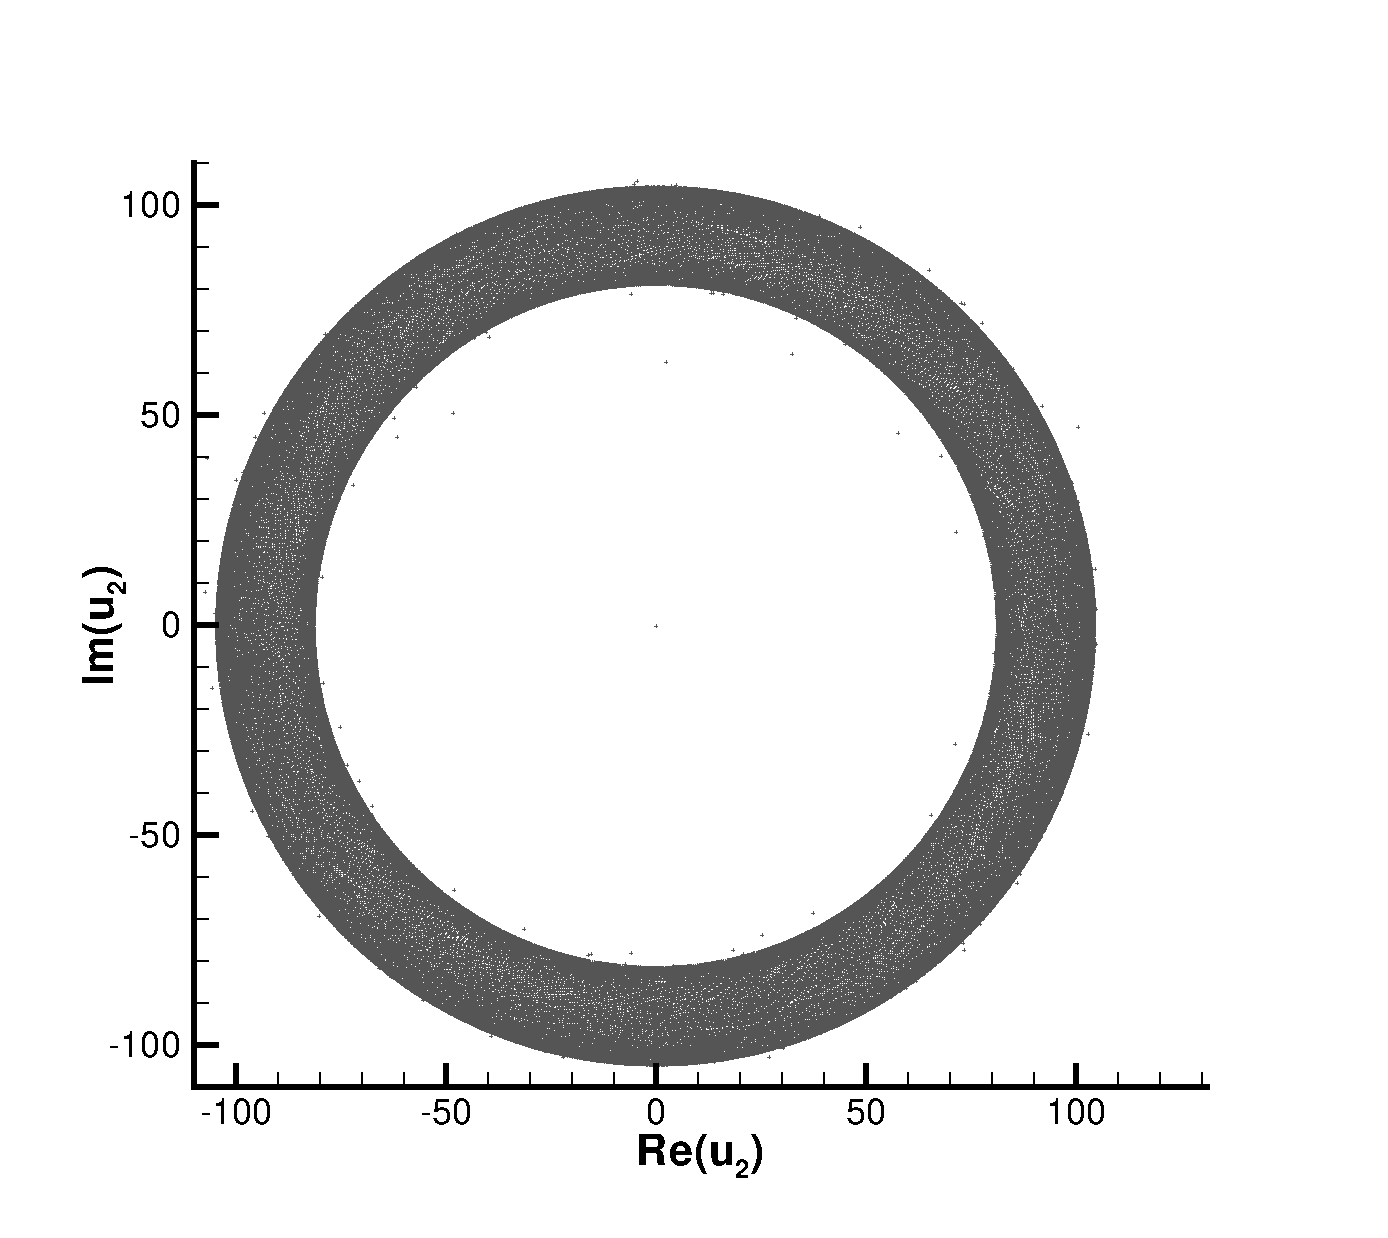
\includegraphics[width=4in]{ns_run10urui.eps}
    \end{center}
    \caption{Distribution of $u_i$. This plot displays the quasi-periodic nature of Run 3 for shell 10 (eps file).} \label{fig: circ symtrc}
\end{figure}

In order to obtain an inertial range which the new similarity theory requires, we increase the forcing for Run 4.  In Run 4, we still have virtually no inertial range.  We must increase the forcing further.  In Run 5, the model is chaotic and we have somewhat more of an inertial range.  Run 6 increases the forcing and the shell number, however we are not obtaining enough of an inertial range. In Run 7, we increase the forcing significantly.  The number of shells remains the same, but this time, we observe a distinct inertial range.  We want to observe how much forcing we can pump into the system before numerical problems arise.  Thus, we create Run 8 and Run 9.  Run 10 is at the limit of what is numerically possible with out model.  This run took four days to complete and is the longest run in the computation.  However, this run is not long enough to generate a statically significant ensemble for the smaller shell numbers.  Therefore, we have backed off in the forcing level and simulated a longer time series in Run 9.

%==========================================GOY Table runs=======================================
\begin{table}[!htp]
        \begin{center}
        \caption{Simulations with the GOY shell model with respective parameters. Run 1 uses the original GOY form found in (\ref{eq: classic goy}).  Runs 2-10 use the log polar form of GOY found in (\ref{eq:log polar goy}).}
        \begin{tabular}{||c|c|c|c|c|c|c||} \hline	
        \multicolumn{7}{|c|}{\emph{Types of Runs Considered for Collapse}} \\ \hline \hline
        Run $\#$    &$t_{end}$         &Forcing 			&$\nu$ 	   &$k_{0}$ &Forcing Shell &$\#$ Shells\\ \hline \hline
        1 & $2\times10^4$   &$(1+i)\times5\times10^{-3}$   &$10^{-7}$&$2^{-4}$ &$4$ &$22$\\
        2 &$1\times10^{-3}$ &$(1+i)\times2.048\times10^{16}$&$1$ 	   &$1$      &$7$ &$26$\\
        3 &$1\times10^{3}$ &$(1+i)\times10^{5}$		      &$1$	   &$1$	     &$1$ &$20$\\
        4 &$3\times10^{2}$ &$(1+i)\times10^{6}$	          &$1$	   &$1$	     &$1$ &$20$\\
        5 &$5\times10$ &$(1+i)\times10^{7}$		      &$1$	   &$1$	     &$1$ &$20$\\
        6 &$1\times10$ &$(1+i)\times10^{8}$  	      &$1$ 	   &$1$      &$1$ &$23$\\
        7 &$1\times10^{-3}$ &$(1+i)\times10^{12}$  	      &$1$ 	   &$1$      &$1$ &$23$\\
        8 &$1\times10^{-6}$ &$(1+i)\times10^{16}$  	      &$1$ 	   &$1$      &$1$ &$27$\\
        9 &$1\times10^{-8}$ &$(1+i)\times10^{20}$  	      &$1$     &$1$      &$1$ &$30$\\
        10&$1\times10^{-10}$ &$(1+i)\times10^{23}$	          &$1$	   &$1$      &$1$ &$36$\\
         \hline \hline
        \end{tabular}
        \end{center}
        \label{table: app GOY table}
\end{table}
%===============================================================================================


\section{Description of Sabra Shell Model Runs and Table}

Like the GOY shell model, the Sabra shell models are forced in the first shell so that the inertial range forms on the ultraviolet side.  However, in run 2 from Table \ref{table: app Sabra table}, forces in shell seven and we are able to observe an infra-red inertial range form. Run 1 uses the parameters of \cite{Yamada} originally used.  This run is used to illustrate the immediate differences between GOY and Sabra, i.e. oscillations in the inertial range.  Figure \ref{fig: ns_sfp} illustrates this.  Run 2 is equivalent to Run 1 in log polar form. The parameters are equivalent to \cite{Yamada} in the original evaluation.  However, in this run, we force in shell 7.  As a result, we see an infra-red inertial range. The affine collapse can be applied to this data as well.  The rest of the runs follow much the same as the GOY shell model.  We again focus on Run 9 for the same reasons as GOY.

%==========================================Sabra Table runs=======================================
\begin{table}[!htp]
        \begin{center}
        \caption{Simulations with the Sabra shell model with respective parameters. Run 1 uses the original Sabra form found in (\ref{eq:sabra}).  Runs 2-10 use the log polar form of Sabra found in (\ref{eq: log polar sabra}).}
        \begin{tabular}{||c|c|c|c|c|c|c||} \hline	
        \multicolumn{7}{|c|}{\emph{Types of Runs Considered for Collapse}} \\ \hline \hline
        Run $\#$    &$t_{end}$         &Forcing 			&$\nu$ 	   &$k_{0}$ &Forcing $n$ &$\#$ of $n$\\ \hline \hline
        1 &$2\times10^4$   &$(1+i)\times5\times10^{-3}$   &$10^{-7}$&$2^{-4}$ &$4$ &$22$\\
        2 &$1\times10^{-3}$ &$(1+i)\times2.048\times10^{16}$&$1$ 	   &$1$      &$7$ &$26$\\
        3 &$1\times10^{3}$ &$(1+i)\times10^{5}$		      &$1$	   &$1$	     &$1$ &$20$\\
        4 &$3\times10^{2}$ &$(1+i)\times10^{6}$	          &$1$	   &$1$	     &$1$ &$20$\\
        5 &$5\times10$ &$(1+i)\times10^{7}$		      &$1$	   &$1$	     &$1$ &$20$\\
        6 &$1\times10$ &$(1+i)\times10^{8}$  	      &$1$ 	   &$1$      &$1$ &$23$\\
        7 &$1\times10^{-3}$ &$(1+i)\times10^{12}$  	      &$1$ 	   &$1$      &$1$ &$23$\\
        8 &$1\times10^{-6}$ &$(1+i)\times10^{16}$  	      &$1$ 	   &$1$      &$1$ &$27$\\
        9 &$1\times10^{-8}$ &$(1+i)\times10^{20}$  	      &$1$     &$1$      &$1$ &$30$\\
        10&$1\times10^{-10}$ &$(1+i)\times10^{23}$	          &$1$	   &$1$      &$1$ &$36$\\
         \hline \hline
        \end{tabular}
        \end{center}
        \label{table: app Sabra table}
\end{table}
%=============================================================================================== 
%\input{app2.tex}

%===================================================================
%   Bibliography goes here
%===================================================================

\bibliographystyle{acm}
\bibliography{proposal_pcui}

\end{thesis}

\end{document}
